\documentclass[12pt]{article}
\usepackage[utf8]{inputenc}
\usepackage[english]{babel}
\usepackage{graphicx}
\usepackage{braket}
\graphicspath{{imagenes/}}
\usepackage{amsmath}
\usepackage{enumerate}
\usepackage{ dsfont }
\usepackage{ mathrsfs }
\usepackage{bbold}
\usepackage{ amssymb }
\usepackage{dsfont}
\usepackage{ mathrsfs }
\usepackage{centernot}
\usepackage{mathtools}
\usepackage{ stmaryrd }
\usepackage{physics}
\usepackage{titlesec}
\usepackage{geometry}
\usepackage{mathtools}
\usepackage{bbold}
\usepackage{caption}
\usepackage{cancel}
\usepackage{subcaption}
\renewcommand{\baselinestretch}{1.3}
\geometry{
 letterpaper,
 left=20mm, right=20mm,
 top=20mm,bottom=21mm
 }


\begin{document}
\begin{center}


\includegraphics[width=2cm]{logo.png}\\

\vspace{2cm}
\textbf{{\LARGE Modeling of Charge Transport for an Artificial Synapse based on Magnetic Josephson Junctions }}\\
\vspace{2.5cm}
{\LARGE{This Dissertation is Submitted for the Degree of}}\\
\vspace{1.0cm}
\centering
{\LARGE{Physicist}}\\
\vspace{2.0cm}
{\large Cristian Mauricio Borja Peña}\\
\vspace{2.5cm}
Universidad de los Andes\\
Faculty of Science\\
Physics Department\\
\vspace{2.5cm}
Bogotá D.C.\hspace{0.1cm}Colombia\\
2018
\newpage
\thispagestyle{empty}

\includegraphics[width=2cm]{logo.png}\\
\vspace{2cm}
\textbf{{\LARGE Modeling of Charge Transport for an Artificial Synapse based on Magnetic Josephson Junctions}}\\
\vspace{1.5cm}
{\LARGE{This Dissertation is Submitted for the Degree of}}\\
\vspace{1.0cm}
\centering
{\LARGE{Physicist}}\\
\vspace{2.0cm}
{\large Cristian Mauricio Borja Peña}\\
\vspace{2.5cm}
Universidad de los Andes\\
Faculty of Science\\
Physics Department\\
\vspace{1.5cm}
Advisor\\
\textbf{\large{Ferney Rodríguez. Ph.D}}\\
\vspace{0.5cm}
Bogotá D.C.\hspace{0.1cm}Colombia\\
2018
\end{center}


\hspace{0pt}
\pagebreak
\clearpage
\tableofcontents
\clearpage


\section{Introduction}

Nowadays, technological advances have been slowed down because of the quantum limitations when the size of transistors and electronic devices are reduced. This has become one of the main concerns in the last decades and various alternatives have been proposed. Neuromorphic Computing promises to improve certain computational tasks as pattern recognition, deep learning and even understand how our brain works.\\

The lastest advances in this field are related to the use of new architectures based on our brain neural networks and the way they facilitate the transport of information. In the NIST (National Institute of Standards and Technology), a new artificial synapse was proposed. The synapse is based on magnetic Josephson junctions, with Nb superconducting electrodes and a barrier composed of Mn nanoclusters between layers of silicon. These devices have been shown to be more energy-efficient than the human brain, requiring activation energies three orders of magnitude below the consumption per synaptic event in the human brain \cite{MAINREF}. In addition, when many devices are connected, the system shows plasticity properties that are similar to the brain ones which at the same time, facilitates and fast the transmission of signals from a neural device to another.\\

The device can be controlled in a relatively simple way due to the superconducting critical current dependency of the order parameter of the Mn nanoclusters. Modelling the response of the device under a current supply in terms of the voltage measured through the junction could be useful to understand how the system behaves under new conditions and therefore, make predictions and test its performance when external parameters are modified (e.g. temperature). When the device was in early development, Russek et al. \cite{RUSSEK} proposed a model to simulate the Voltage-Current response of the synapse and how the stochastic operation of this device could be useful for future applications. \\

In this work, we study the charge transport in the synapse-device proposed by Schneider et al. \cite{MAINREF}. The Russek model, a modified Josephson junction standard circuit model, was studied and results of the stochastic operation were reproduced. On the other hand, following Xin-Qi Li and YiJing Yang \cite{CORRIENTES} we explore a Tight Binding Model combined with the Landauer formalism in order to verify if this simple model can describe the charge transport in the synapse. Although this simple model is not directly related to the superconductivity phenomena, it is usual treat this kind of transport problems with lattice models based on this methodology. For this reason, study Tight Binding model is a first step to propose an alternate model that can explain the device operation.
 
 
\section{About the Device}

\subsection{Structure}
The device is composed of two superconducting Niobium electrodes. Between the electrodes there is Silicon barrier with a series of layers of Manganese spin nanoclusters. The device was measured in a liquid He flow at 3.9K$\pm$5mK.  

\begin{figure}[ht]
    \centering
     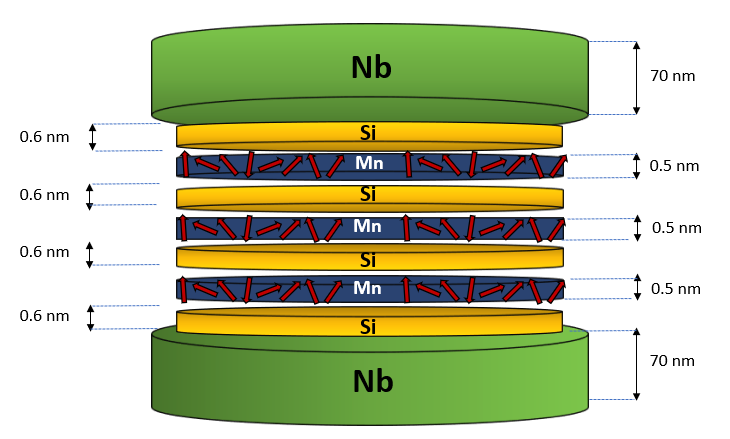
\includegraphics[scale=0.5]{Device.png}
    \caption{Device structure illustration.}
    \label{Device}
\end{figure}

The device has a blocking temperature of 52$\pm$2K. With this information, the size of the nanoclusters was estimated $2\times 10^{4}$ Mn clusters$/\mu m^{2}$ and each cluster with $2000\pm 100 \mu_{B}$ (the Bohr magneton).

\subsection{Operation}
As said before, the device shows to be controlled by varying external parameters as magnetic field, temperature and electric pulse trains. The device can operate in two states depending on the current applied: a superconducting state and a voltage state. In the superconducting state, the voltage measured through the junction is zero until the applied current surpass the value of the superconducting critical current.  \\

Generally, the value of the critical current depends on the superconducting material used in the device, however the experimental results shows that when a magnetic layer is between the two superconducting electrodes, the critical current also depends on the order parameter of the magnetic layer and the temperature. The superconducting critical current value, experimentally can be reduced by means of the application of electrical pulses and a constant applied magnetic field. The effect can be reversed by applying electrical pulses but turning off the magnetic field.\\

\begin{figure}[ht]
    \centering
    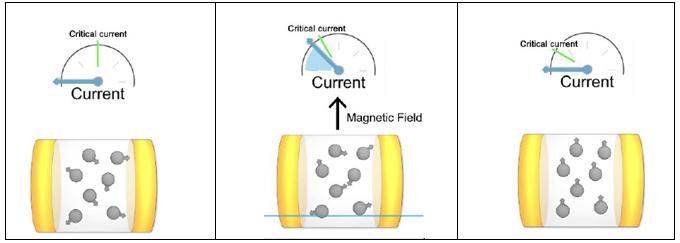
\includegraphics[scale=0.75]{CurrentBehavior.png}
    \caption{Illustration of the mechanism of signal transmission through the junction. Taken from NIST Animation \cite{NISTIlus}}
    \label{CurrentBehave}
\end{figure}


In the superconducting state, as voltage is zero, no signal can pass through the junction. When the critical current is surpass, the system enters into the voltage state, where a voltage spike train\footnote{This voltage spike train is called SFQ or Single Flux Quantum} is measure through the junction, which implies that signals can be transmitted from a neural device to another (see Figure \ref{CurrentBehave}).  \\

The control of the system can be accomplished if we vary the energy needed to switch the system to the voltage state by modifying the order state of the Mn nanoclusters. A magnetically ordered state correspond to a low superconducting critical current and hence, a low energy is require to bring the system to the voltage state. In summary, we can modify the energy needed to transmit a signal through the junction and hence we can control when the synapse allow or not communication between neural devices. This behavior can be seen in Figure \ref{VI}.\\


\begin{figure}[ht]
    \centering
     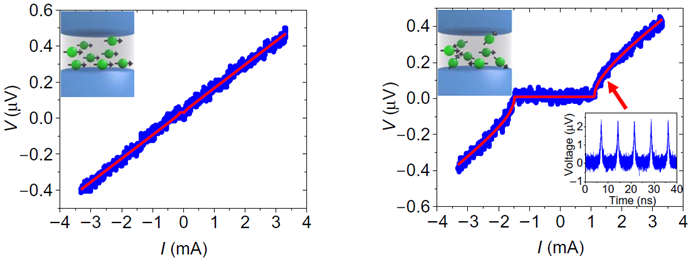
\includegraphics[scale=0.8]{CurveVI.png}
    \caption{Current-voltage characteristic of the device in the ordered and disordered states. (Taken from the results of Schneider et al. \cite{MAINREF}). (Left) VI curve (Ordered State). (Right) VI curve (Disordered State). The data is fit to the RSJ model.}
    \label{VI}
\end{figure}

As can be seen in Figure \ref{VI}. (Left) in the ordered state, experimentally there is a small amount of \textit{disorder} that cannot be suppressed (note that there is a small current at zero voltage). On the other hand, in the disordered state(Right), the current range in which the system is out of the voltage state is bigger because of the high superconducting critical current value.\\

Low temperature is needed in order to take advantage of the superconducting Josephson effect, however maintain a stable temperature require a higher energetic cost. Russek \cite{RUSSEK} proposed to allow thermal fluctuations and use this stochasticity to mimic our natural brain operation. The simulations made by Russek, shows that stochasticity (associated to thermal noise) can affect the output voltage spiking and the variation of the order parameter when the temperature is increased. This offers an alternate way to control the synapse and at the same time, reduces the energy cost of the thermal stabilization.

\clearpage
\newpage
\section{Theoretical Framework}

 In order to approach the main problem of this dissertation, in this section will be presented the elementary theory that is used to develop the proposed models. Tight binding model combined with the Landauer formalism describes charge transport by imposing a gradient of chemical potential between two electron reservoirs. In this model, additional effects on the system can be considered coupling the chain to probe electrodes. \\
 
 On the other hand, a background in Josephson effect is required to understand how the artificial synapse works and it is useful when we study the Russek model \cite{RUSSEK} (a modified standard circuit model for Josephson Junctions that fits the current-voltage characteristic of the device developed by Schneider et al. \cite{MAINREF}).  

\clearpage
\newpage
\subsection{Josephson Effect}




\clearpage
\newpage
\subsection{Tight Binding Model}

\begin{figure}[ht]
    \centering
    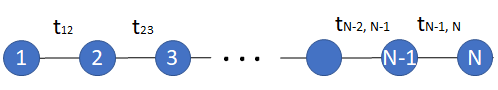
\includegraphics[scale=0.7]{TightBindingChain.png}
    \caption{Tight Binding chain representation.}
    \label{Chain}
\end{figure}

 The (1D) Tight Binding Model or Nearly Free Electron Model describes the physics of a 1D chain of N sites, each one with a molecular potential $U_{i}$. Each site $i$ interacts with its nearest neighbour by means of a hopping term $t$. The Hamiltonian that describes a system of N sites is given by the equation:
 
\begin{equation}\label{TBH}
 \textbf{H} = \sum_{n=1}^{N}(U_{n}+2t)\ket{n}\bra{n} -t(\ket{n}\bra{n+1}) - t(\ket{n+1}\bra{n})
\end{equation}
 
Where $U_{n}$ denotes the site-potentials of the nth-site and $t$ is the hopping term. The matrix representation of this Hamiltonian can be written as: 
\\
\[\left(
	\begin{matrix}
	U_{1}+2t & -t & 0 & \hdots & \\
	-t & U_{2}+2t & -t & \hdots & \\
	0 & -t & U_{3}+2t & \hdots & \\
	\vdots & \vdots & \vdots &\ddots & \\
	& & & & U_{N}+2t
	\end{matrix} 
	\right)
	\left(
	\begin{array}{c}
    	\psi_{1}  \\
    	\psi_{2} \\
    	\psi_{3} \\
    	\vdots  \\
    	\psi_{N}
	\end{array}
	\right) 
	= E \left(\begin{array}{c}
	    \psi_{1}  \\
 	   	\psi_{2} \\
	    \psi_{3} \\
 	   	\vdots  \\
 	   \psi_{N}
	\end{array}
\right)
\]
\\

For the special case in which $U_{1} = \hdots = U_{N}$ are fixed to a value $U_{0}$ and the hopping terms are equal between each pair of sites, the dispersion relation that describes the eigen-energies of the system is:

\begin{equation}\label{DispRel}
	E(k) = U_{0} + 2t(1-\cos(ka))
\end{equation}

Where $k=\frac{n\pi}{a}$, $a$ is the distance between the sites of the chain, $n=0,1,2, \hdots$ and $E_{0} = U_{0}+2t$ is defined as the on-site energy. On the other hand, the density of states can be obtained from the previous expression as:

\begin{equation}\label{DoS}
	N(E) = \frac{dN}{dE(k)} = \frac{dN}{dk}\frac{dk}{dE(k)} = \frac{1}{4\pi t} \frac{1}{\sqrt{1-\left(\frac{E-E_{0}}{2t}\right)^{2}}}    
\end{equation}

\subsection{Landauer Formalism}

Given an energy spectrum, in this case from the Tight Binding model, Landauer formalism allow us to calculate a current response associated to the transport of electrons through the chain of sites when we consider a gradient of chemical potential. First, it is necessary to calculate the transmission functions across the chain using the energy spectrum from Tight Binding matrix. Then we consider that a voltage is applied to the chain and we calculate the current response for each voltage value. 

\subsubsection{Transmission function calculation}
 In order to calculate currents for the model, following Xin-Qi Li and YiJing Yang  \cite{CORRIENTES}, it is necessary to know the transmission function. First we have to consider that the chain of N-sites is coupled to a pair of electron reservoirs (Left and Right), the difference of potential between the reservoirs is what generates the current. 

\begin{figure}[ht]
    \centering
    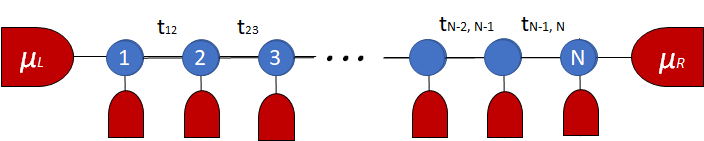
\includegraphics[scale=0.65]{ReservoirsCoupling.png}
    \caption{TB chain coupled to reservoirs representation.}
    \label{CoupledChain}
\end{figure}

To consider the coupling of the chain with the reservoirs it is defined an effective Hamiltonian as the sum of the original TB Hamiltonian and a matrix that describes the coupling:

\begin{equation}\label{Heff}
	H_{eff} = \textbf{H} + \Sigma_{L}\ket{1}\bra{1} + \Sigma_{R}\ket{N}\bra{N} + \sum_{j=1}^{N} \Sigma_{j}\ket{j}\bra{j}
\end{equation}

Where, $Sigma_{\mu}$ are self-energy terms that describes the coupling of the chain with the reservoirs. Those terms are given by:

\begin{equation}\label{self_e}
\Sigma_{\mu} = \frac{V_{\mu}^{2}}{E-E_{\mu}-\sigma_{\mu}}
\end{equation}

Where $V_{\mu}$ is the coupling potential of the reservoir to the chain, $\gamma_{\mu}$ is the hopping term between the chain and the reservoir. $E$ is the Tight Binding eigen-energy for which the transmission function is been calculated, $E_{\mu}$ is the on-site energy ($U_{\mu}+2t$) and $\sigma_{\mu}$ is given by:

\begin{equation}\label{sigma}
\sigma_{\mu} = \left(\frac{E - E_{\mu}}{2}\right) - i\left[ \gamma_{\mu}^{2} - \left(\frac{E - E_{\mu}}{2}\right)^{2} \right]^{1/2}
\end{equation}

Now, the retarded Green function is calculated for a determined TB Hamiltonian energy $E$ as:

\begin{equation}\label{Green}
G(E) = [E \mathds{1} - H_{eff}]^{-1}
\end{equation}

And finally, the transmission coefficient between two reservoirs (i.e. Left and Right) can be written as:

\begin{equation}\label{TLR}
	T_{L,R} = 4\Delta_{L}\Delta_{R}|G(E)|^{2}
\end{equation}

Where:
\begin{equation}\label{ImSigma}
	\Gamma_{\mu} = -Im(\Sigma_{\mu})
\end{equation}

In order to consider the non-coherent transmission, it is required to include another term to the sum. Then, the effective transmission can be written as:

\begin{equation}\label{Teff}
	T_{eff} = T_{L, R} + \sum_{q=1}^{N}\sum_{p=1}^{N} T_{q, R} W_{qp}^{-1} T_{L, p}
\end{equation}

\subsubsection{Currents calculation}

Once defined the transmission function, it is defined a Fermi function for each electron reservoir (Left and Right), this function depends on $V$ the potential difference applied to the chain, a constant $\kappa$ that determines the unbalance of potential between the two reservoirs, the Fermi energy $E_{f}$ of the chain, the Tight Binding Hamiltonian eigen-energies $E$ and the temperature $T$:

$$
	\mu_{L} = E_{f} - \kappa eV
$$
$$
	\mu_{R} = E_{f} + (1 - \kappa) eV
$$

\begin{equation}\label{Fermifunc}
	f_{d}(E, V)= \frac{1}{e^{\frac{E-\mu_{d}}{k_{B}T}+1}}
\end{equation}

Now, the current through the chain can be expressed as:

\begin{equation}\label{Current}
	I(E, V) = \frac{2e}{h}\int_{-\infty}^{\infty} T_{eff}(E)[f_{L}(E, V)-f_{R}(E, V)] dE
\end{equation}


\clearpage
\newpage
\section{One Dimensional Tight Binding Model}
It was developed a computational 1D Tight Binding Model capable of calculate currents by means of Landauer formalism. In the model we generate TB Hamiltonians with different restrictions on the parameters $t$ and $U_{n}$: 

\begin{itemize}
	\item All hopping terms are equal to a chosen constant value and the molecular potentials $U_{n}$ are the same and equal to a constant value (i.e. $U_{1} =  U_{2} = \hdots = U_{N}$).

	\item All hopping terms are equal to a chosen constant value and the molecular potentials $U_{n}$ are different for every site and take random values according to a determined distribution of probability (i.e. $U_{1}\neq U_{2}\neq \hdots \neq U_{N}$)\footnote{As the values of the parameters are chosen randomly according to a distribution, it could be possible that some values are repeated}.

     \item All hopping terms are different between all sites, however the hopping value to go from site $\ket{n}$ to the site $\ket{n+1}$ is the same that the hopping value to go from site to the site $\ket{n}$ such that the Hamiltonian is hermitian (the values are chosen according to a determined distribution of probability). On the other hand, the molecular potentials can be chosen to be different in all sites as described previously or can be fixed to a chosen value.    
\end{itemize}


In order to test the program, the TB Hamiltonian matrix is diagonalized and with the obtained eigen-energies we proceed with the numerical calculation of the energy spectrum and the density of states (DoS). By comparing the numerical calculations with the expected analytical results given by the equations Eq.(\ref{DispRel}) and Eq.(\ref{DoS}) it can be verified that the program works. It is important to clarify that this comparison between analytical and numerical calculations only make sense in the situation where $t$ and $U_{n}$ have been fixed to constant values. This special case is the only one that have a simple analytical solution. 

\subsection{Energy Spectra and Density of States (DoS)}
The analytical solution to the 1D TB Model energies is given by the dispersion relation Eq.(\ref{DispRel}) and the density of states by the equation Eq.(\ref{DoS}).\\

Numerically the energy spectrum is obtained from the diagonalization of the TB Hamiltonian. According to Eq.(\ref{DoS}), in order to compute the DoS it is necessary to calculate the derivative of the energy spectrum ($\frac{dE(k)}{dk}$) and $dN/dk$ is the amount of states that can occupy a space $dk$ (equal to $\frac{1}{2\pi}$). Then, calculating the inverse of the derivative of the energy spectrum multiplied by a factor of $\frac{1}{2\pi}$ we obtain the Density of States.\\

The plot of the analytical and numerical calculations for the Energy Spectrum and the DoS are shown in Figure \ref{f1}. As can be seen, the numerical data fits the analytical predictions for the selected values of $t$ and $U_{0}$.

\begin{figure}[ht]
    \centering
    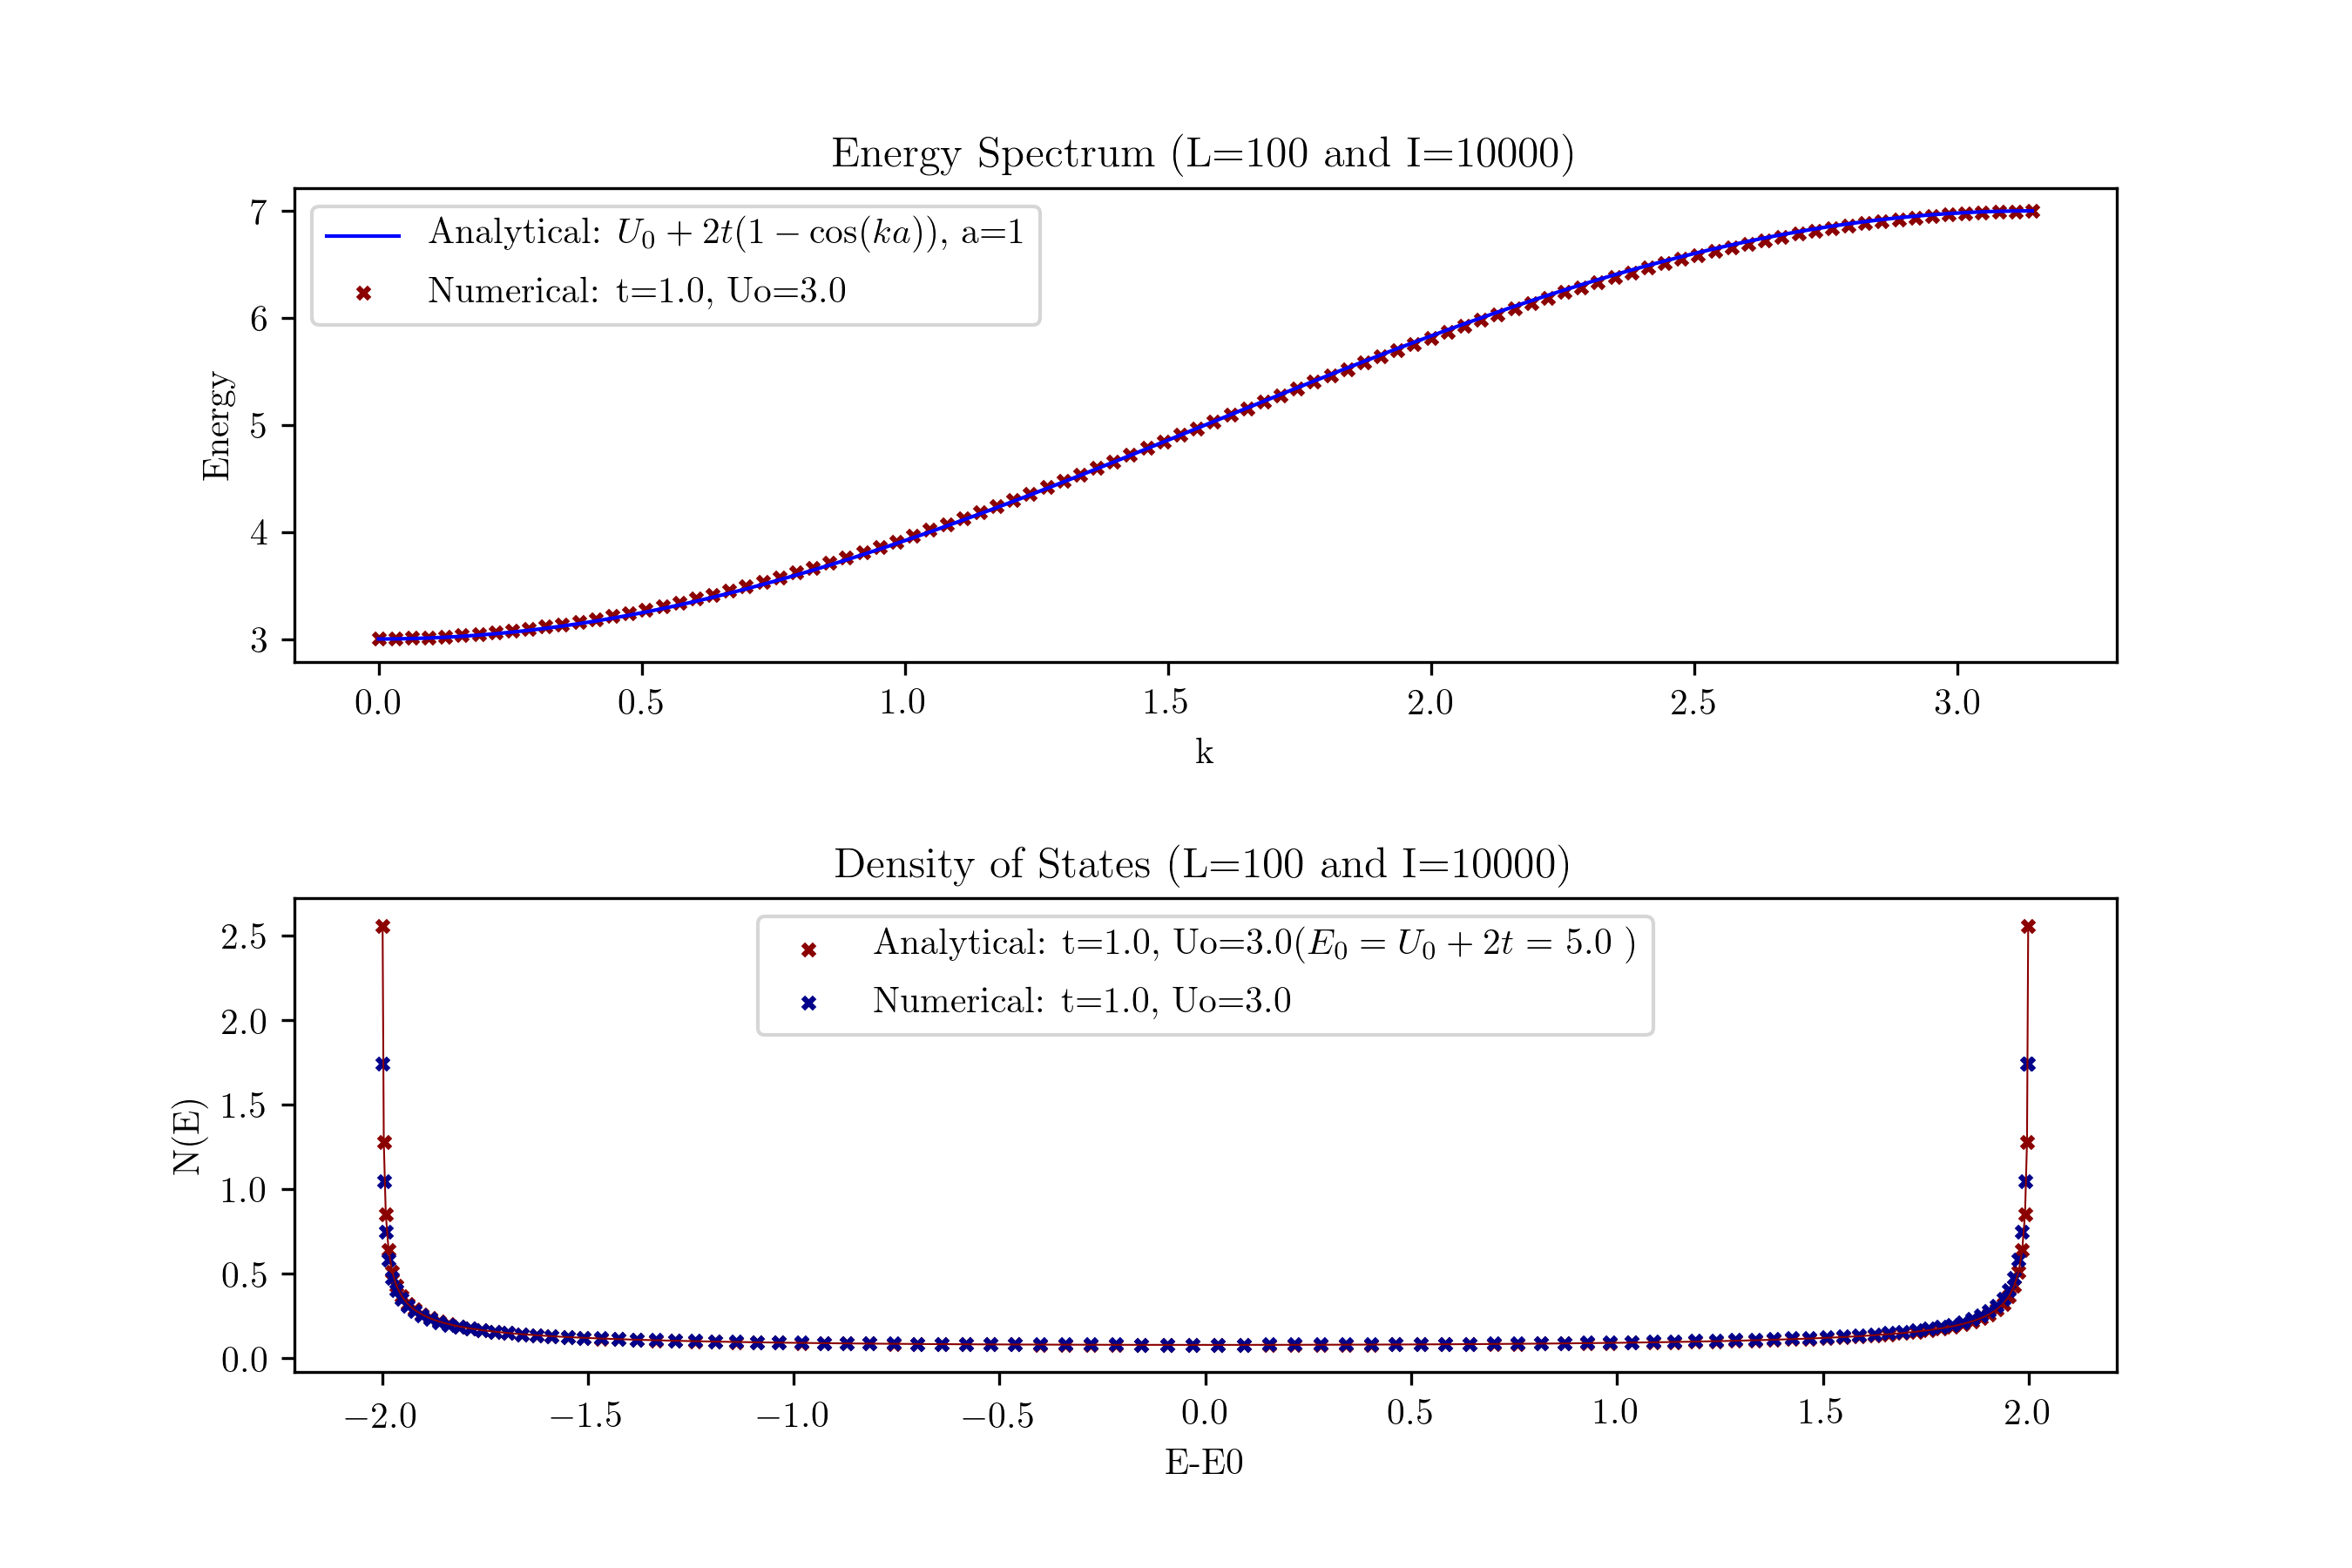
\includegraphics[scale=0.65]{EDOSCC100.png}
    \caption{Analytical vs. Numerical calculation of Energy Spectrum and Density of Sates for a chain of L=100 sites.}
    \label{f1}
\end{figure}

Once the program is tested, we proceed with the calculation of density of states and energy spectrum for another variations of the TB Hamiltonian. In those cases it is obtained an averaged curve from a determined number of iterations of the program and based on that curve the DoS can be computed.

\begin{figure}[ht]
		\centering
        \begin{subfigure}[a]{\textwidth}
        		\centering
                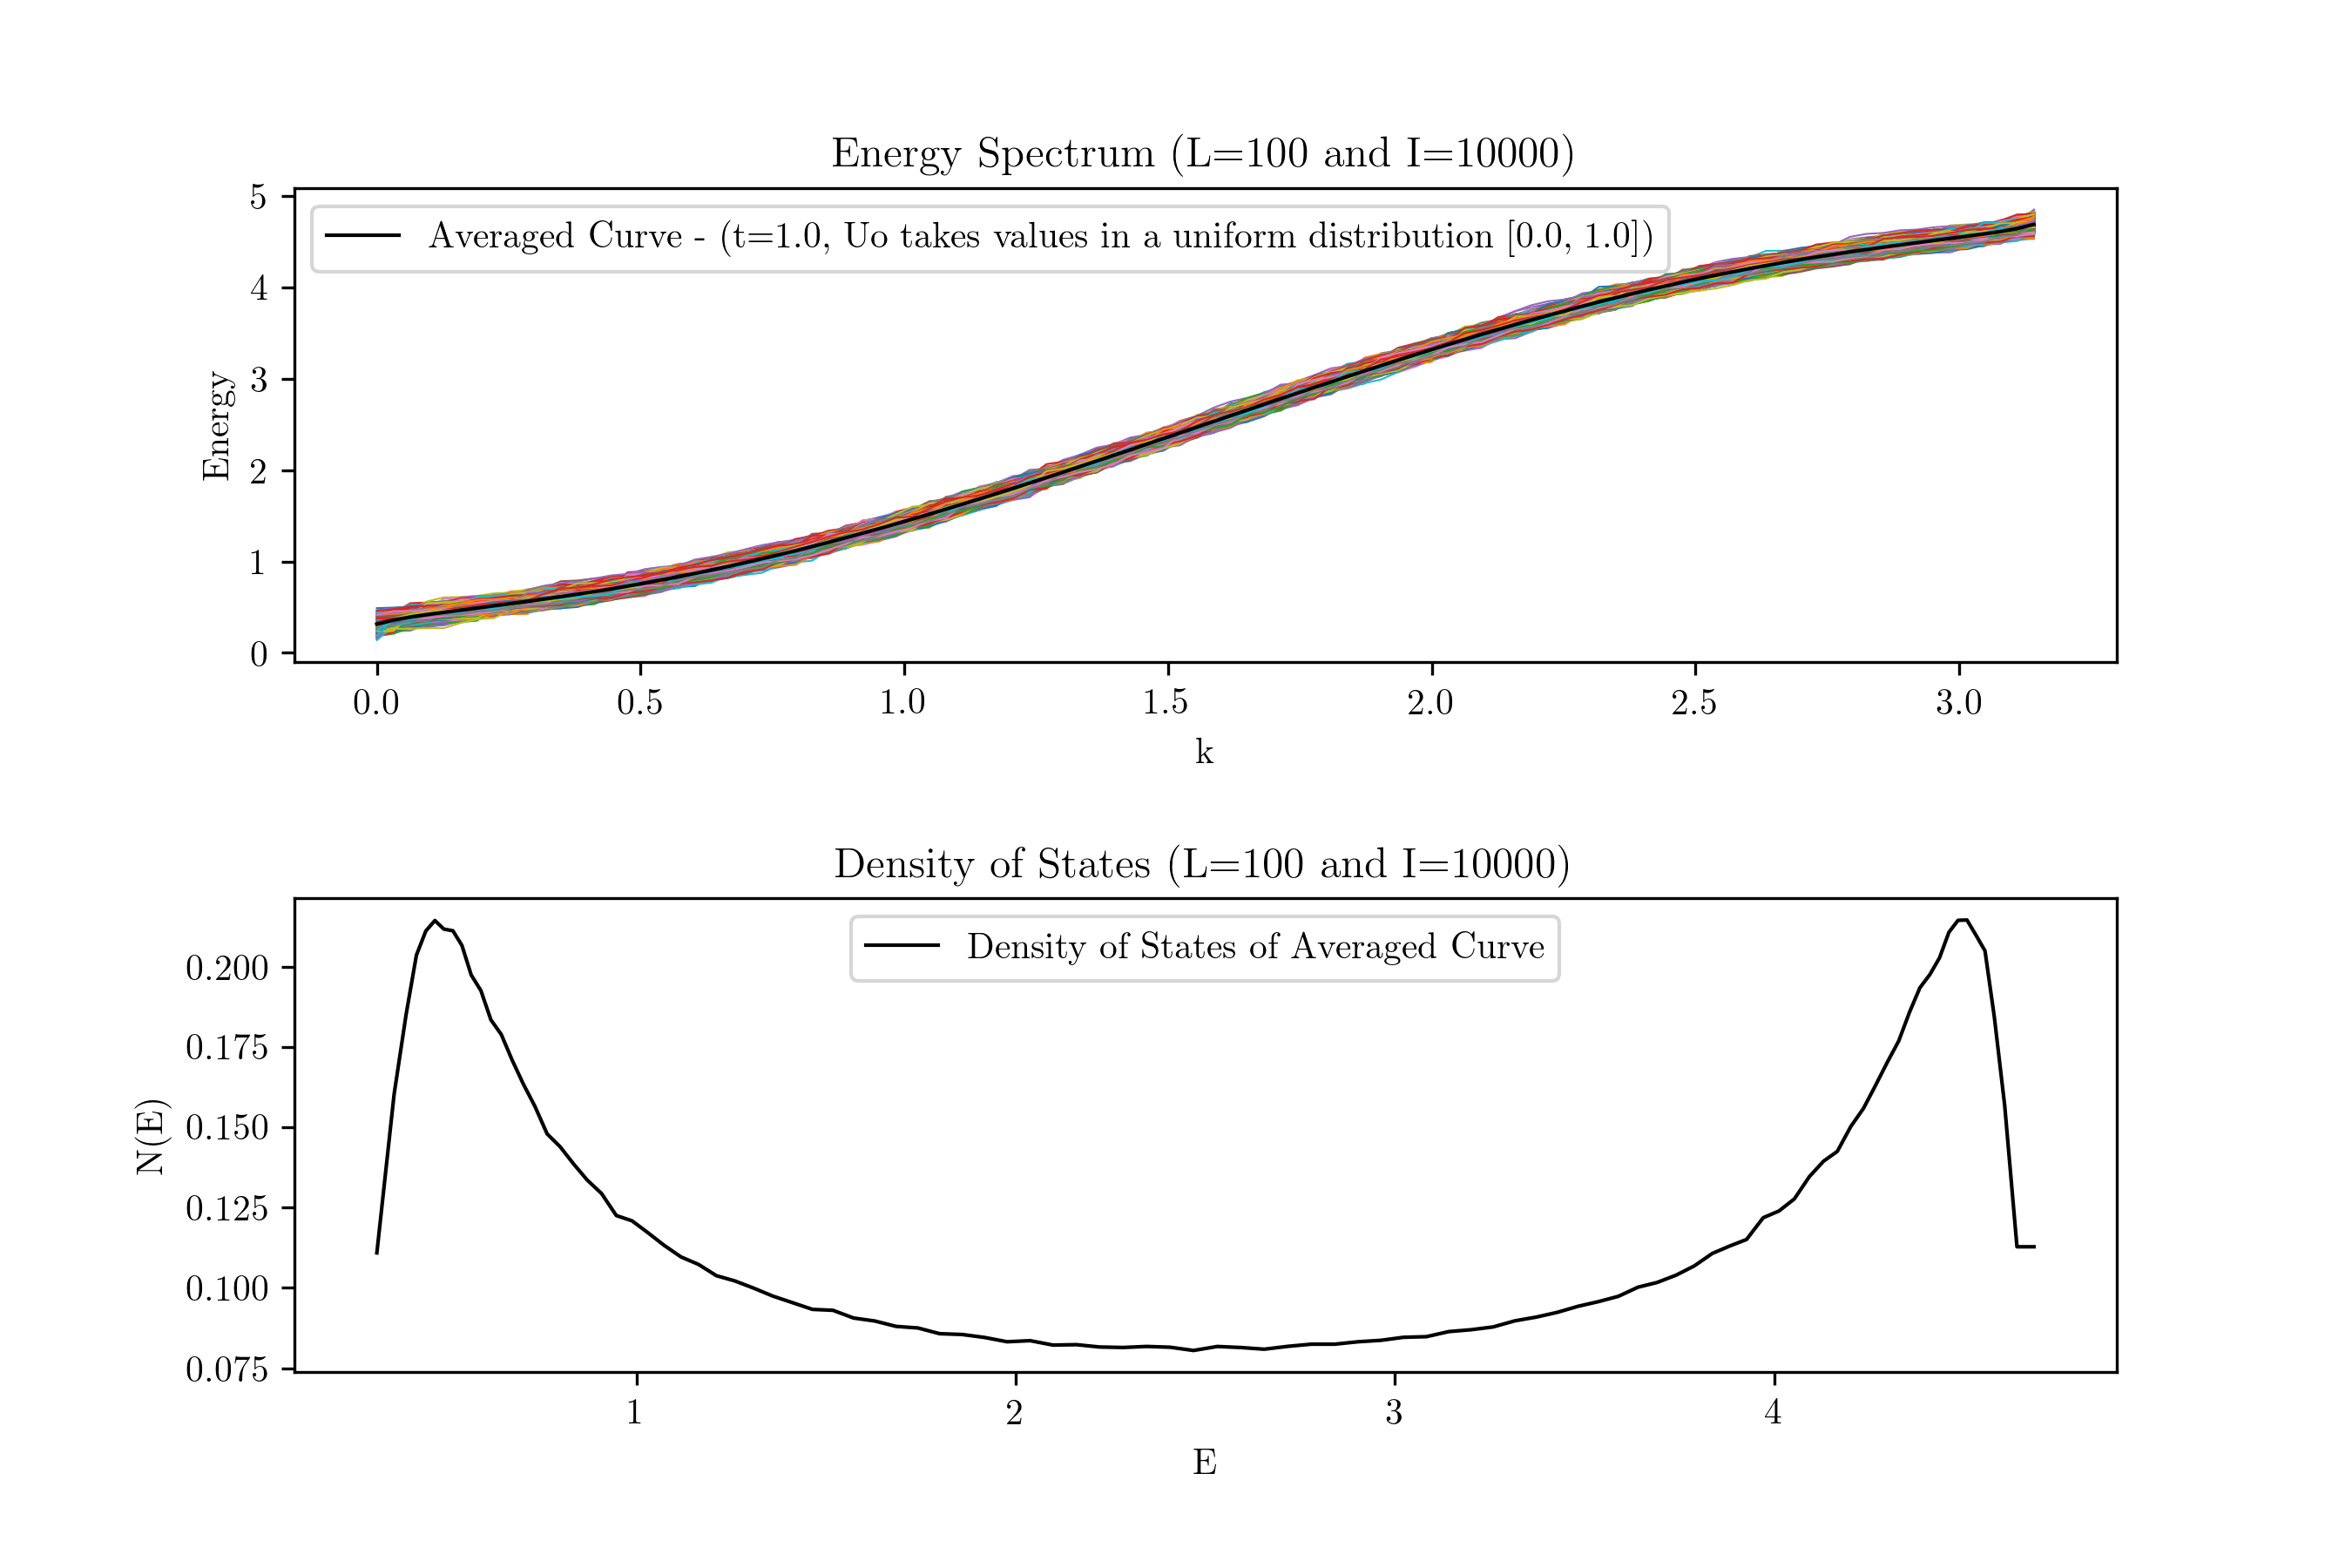
\includegraphics[scale=0.65]{EDOSCRU.png}
                \caption{Energy Spectrum and DoS, on-site potential terms $U_{0}$ take values in a uniform distribution.}
                \label{f2a}
        \end{subfigure}
        \begin{subfigure}[b]{\textwidth}
        		\centering
                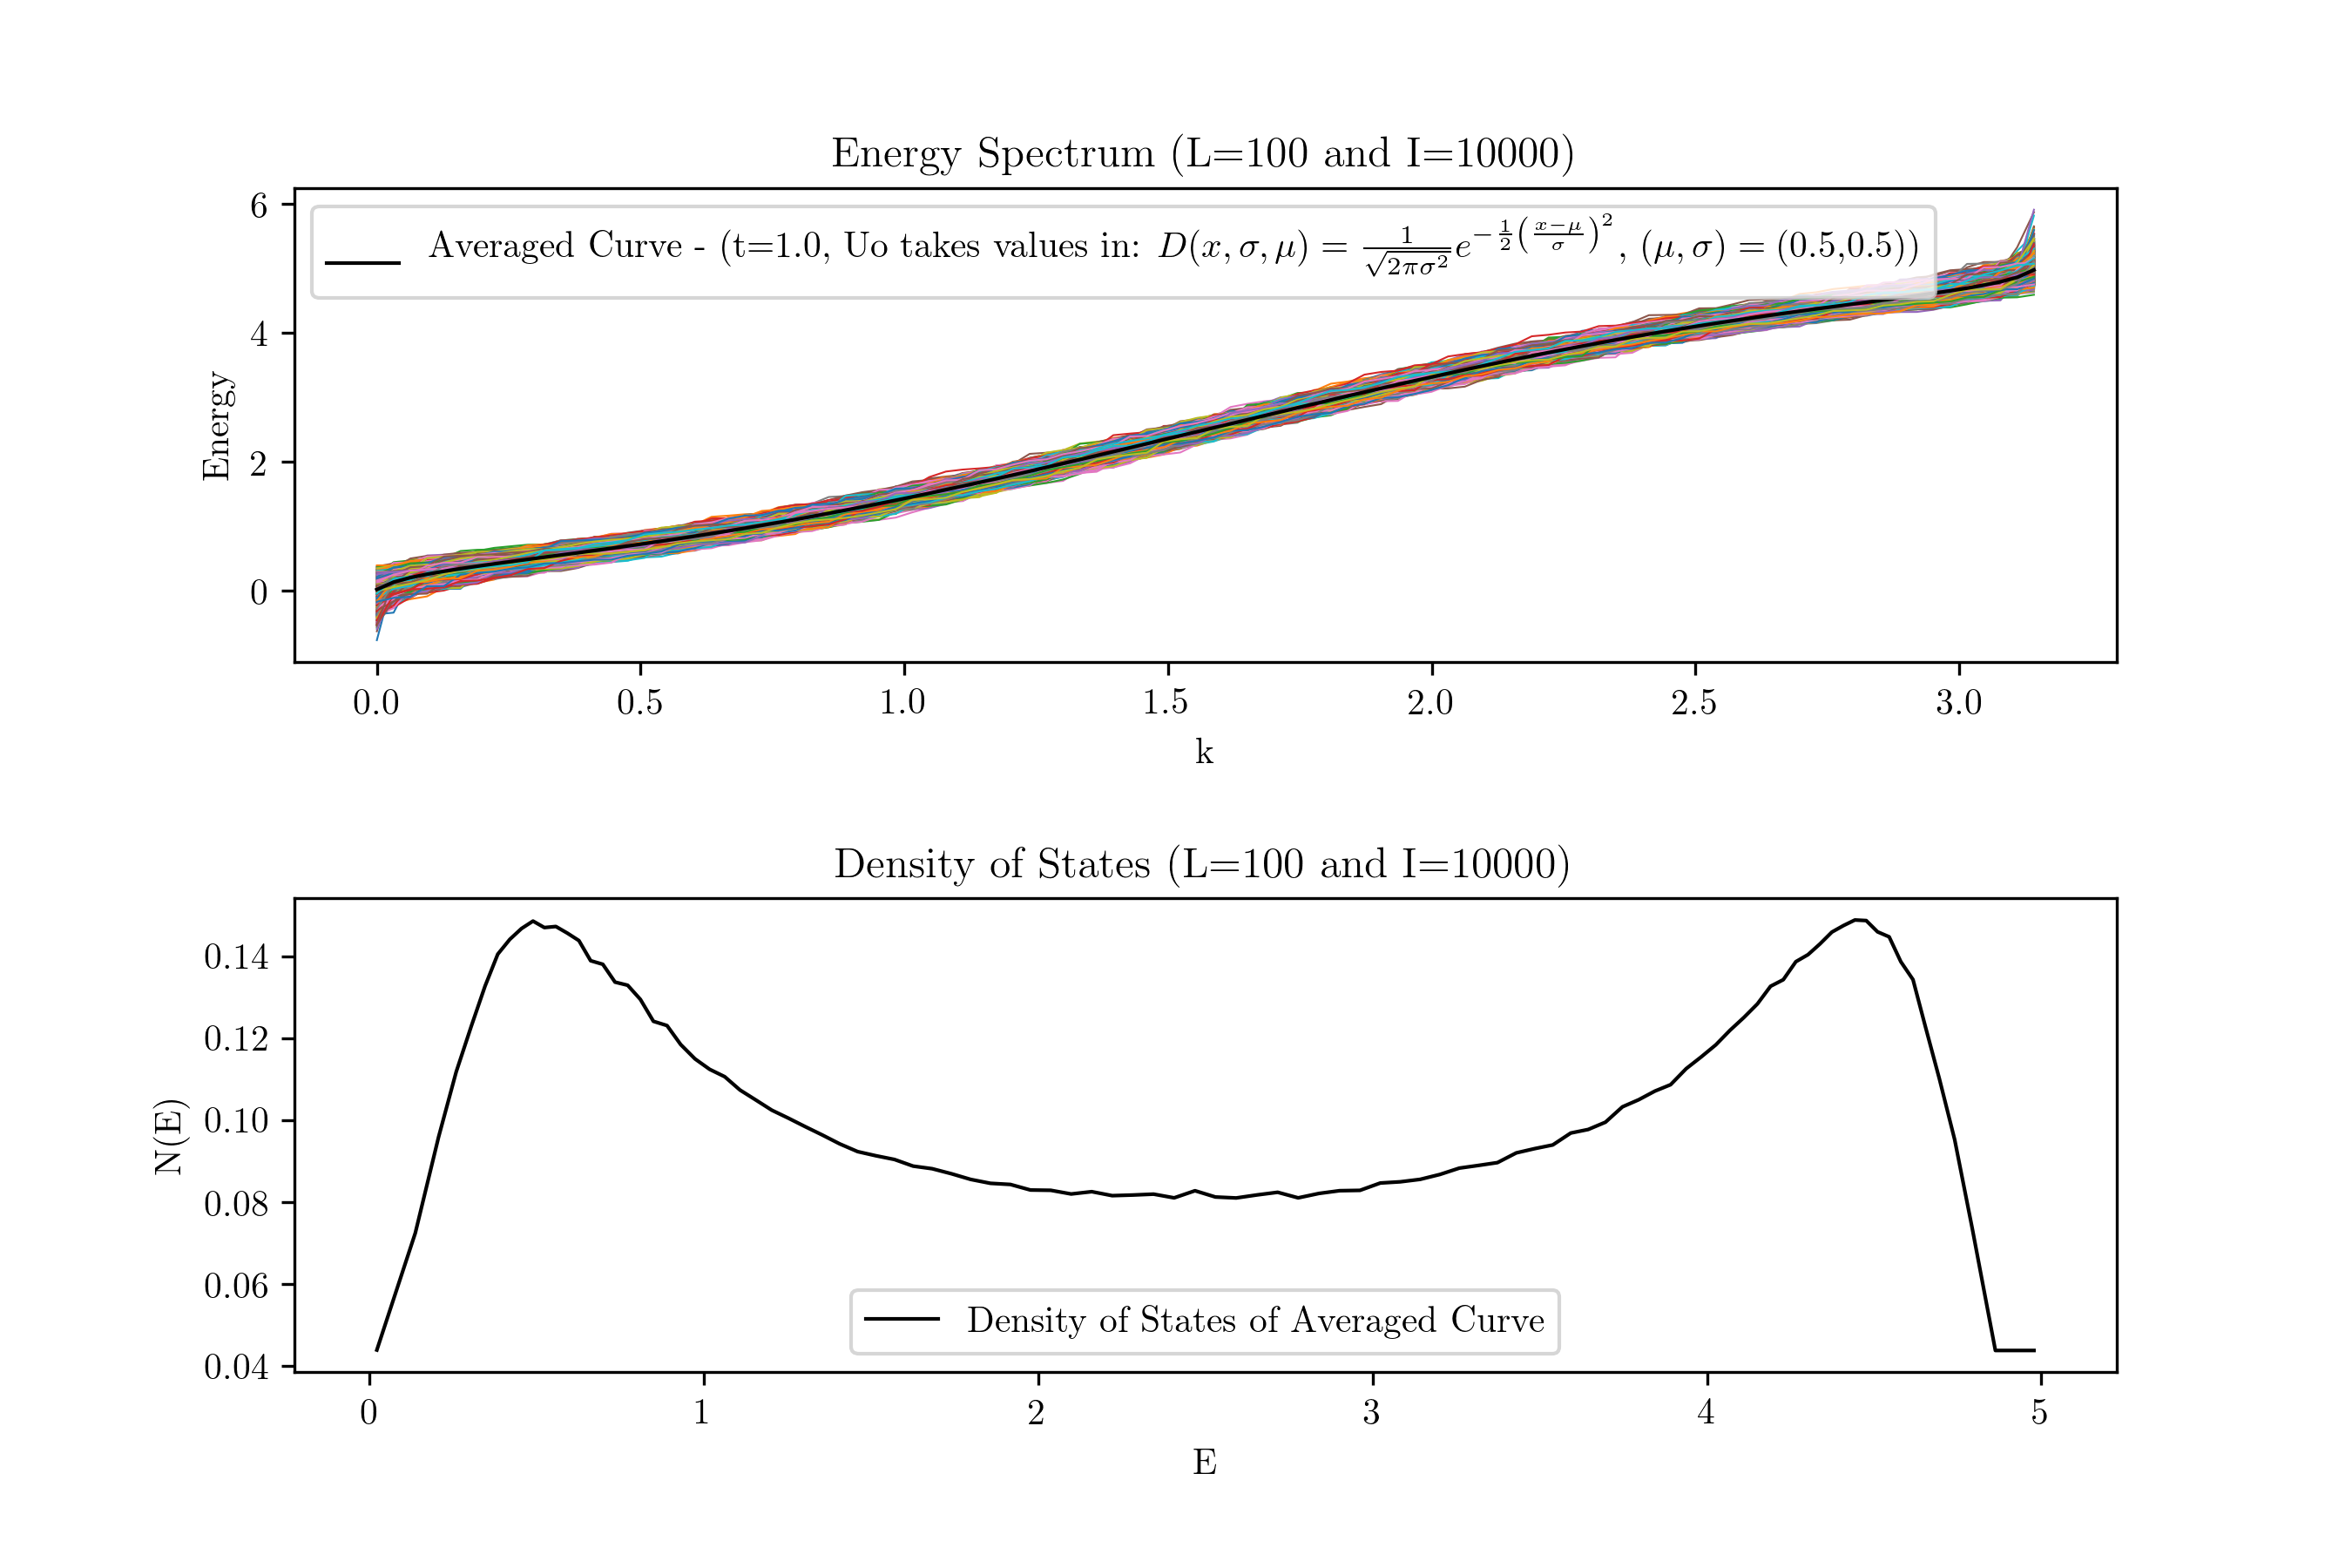
\includegraphics[scale=0.65]{EDOSCRN.png}
                \caption{ Energy Spectrum and DoS, on-site potential terms $U_{0}$ take values in a normal distribution.}
                \label{f2b}
        \end{subfigure}
        \caption{Chain of 100 sites and 10000 iterations, on-site potential terms $U_{0}$ take values in: (a) uniform distribution and (b)  normal distribution.}
        \label{f2}
\end{figure}
An additional test was performed for the TB Hamiltonians whose parameters follow a normal distribution. The width of the peaks of the DoS in Figure \ref{f2}(b) is due to the standard deviation of the Gaussian distribution; in order to verify the convergence of the numerical results to the analytical ones, the expected value $\mu$ was set to be the constant value defined for $U_{0}$ in Figure \ref{f1}. and a very small value of $\sigma$ was used for generating the numbers in the normal distribution. As expected, the numerical calculations converge to the analytical ones.\\


In Figure \ref{f2} and Figure \ref{f3} is shown the energy spectrum and the DoS for the same 100 sites chain and in the case when it is considered a constant value of hopping terms but with the on-site potentials values following certain distributions. On the other hand, Figure \ref{f4} and Figure \ref{f5} show the case in which the on-site potential is the same in all the sites of the chain but the hopping terms take values in a certain distribution.\\


The last case considered (shown in Figure \ref{f6} and Figure \ref{f7})is with the hopping terms following a certain distribution and the $U_{0}$ following the same distribution (the case in which both parameters follows different distributions can be considered in future calculations depending on the interest in consider those special cases). Due to the differences in the DoS distribution in each of the cases shown before, the posterior transmission coefficient calculations may vary\footnote{these calculations have not yet been made.}. 


\begin{figure}[ht]
		\centering
        \begin{subfigure}[a]{\textwidth}
        		\centering
                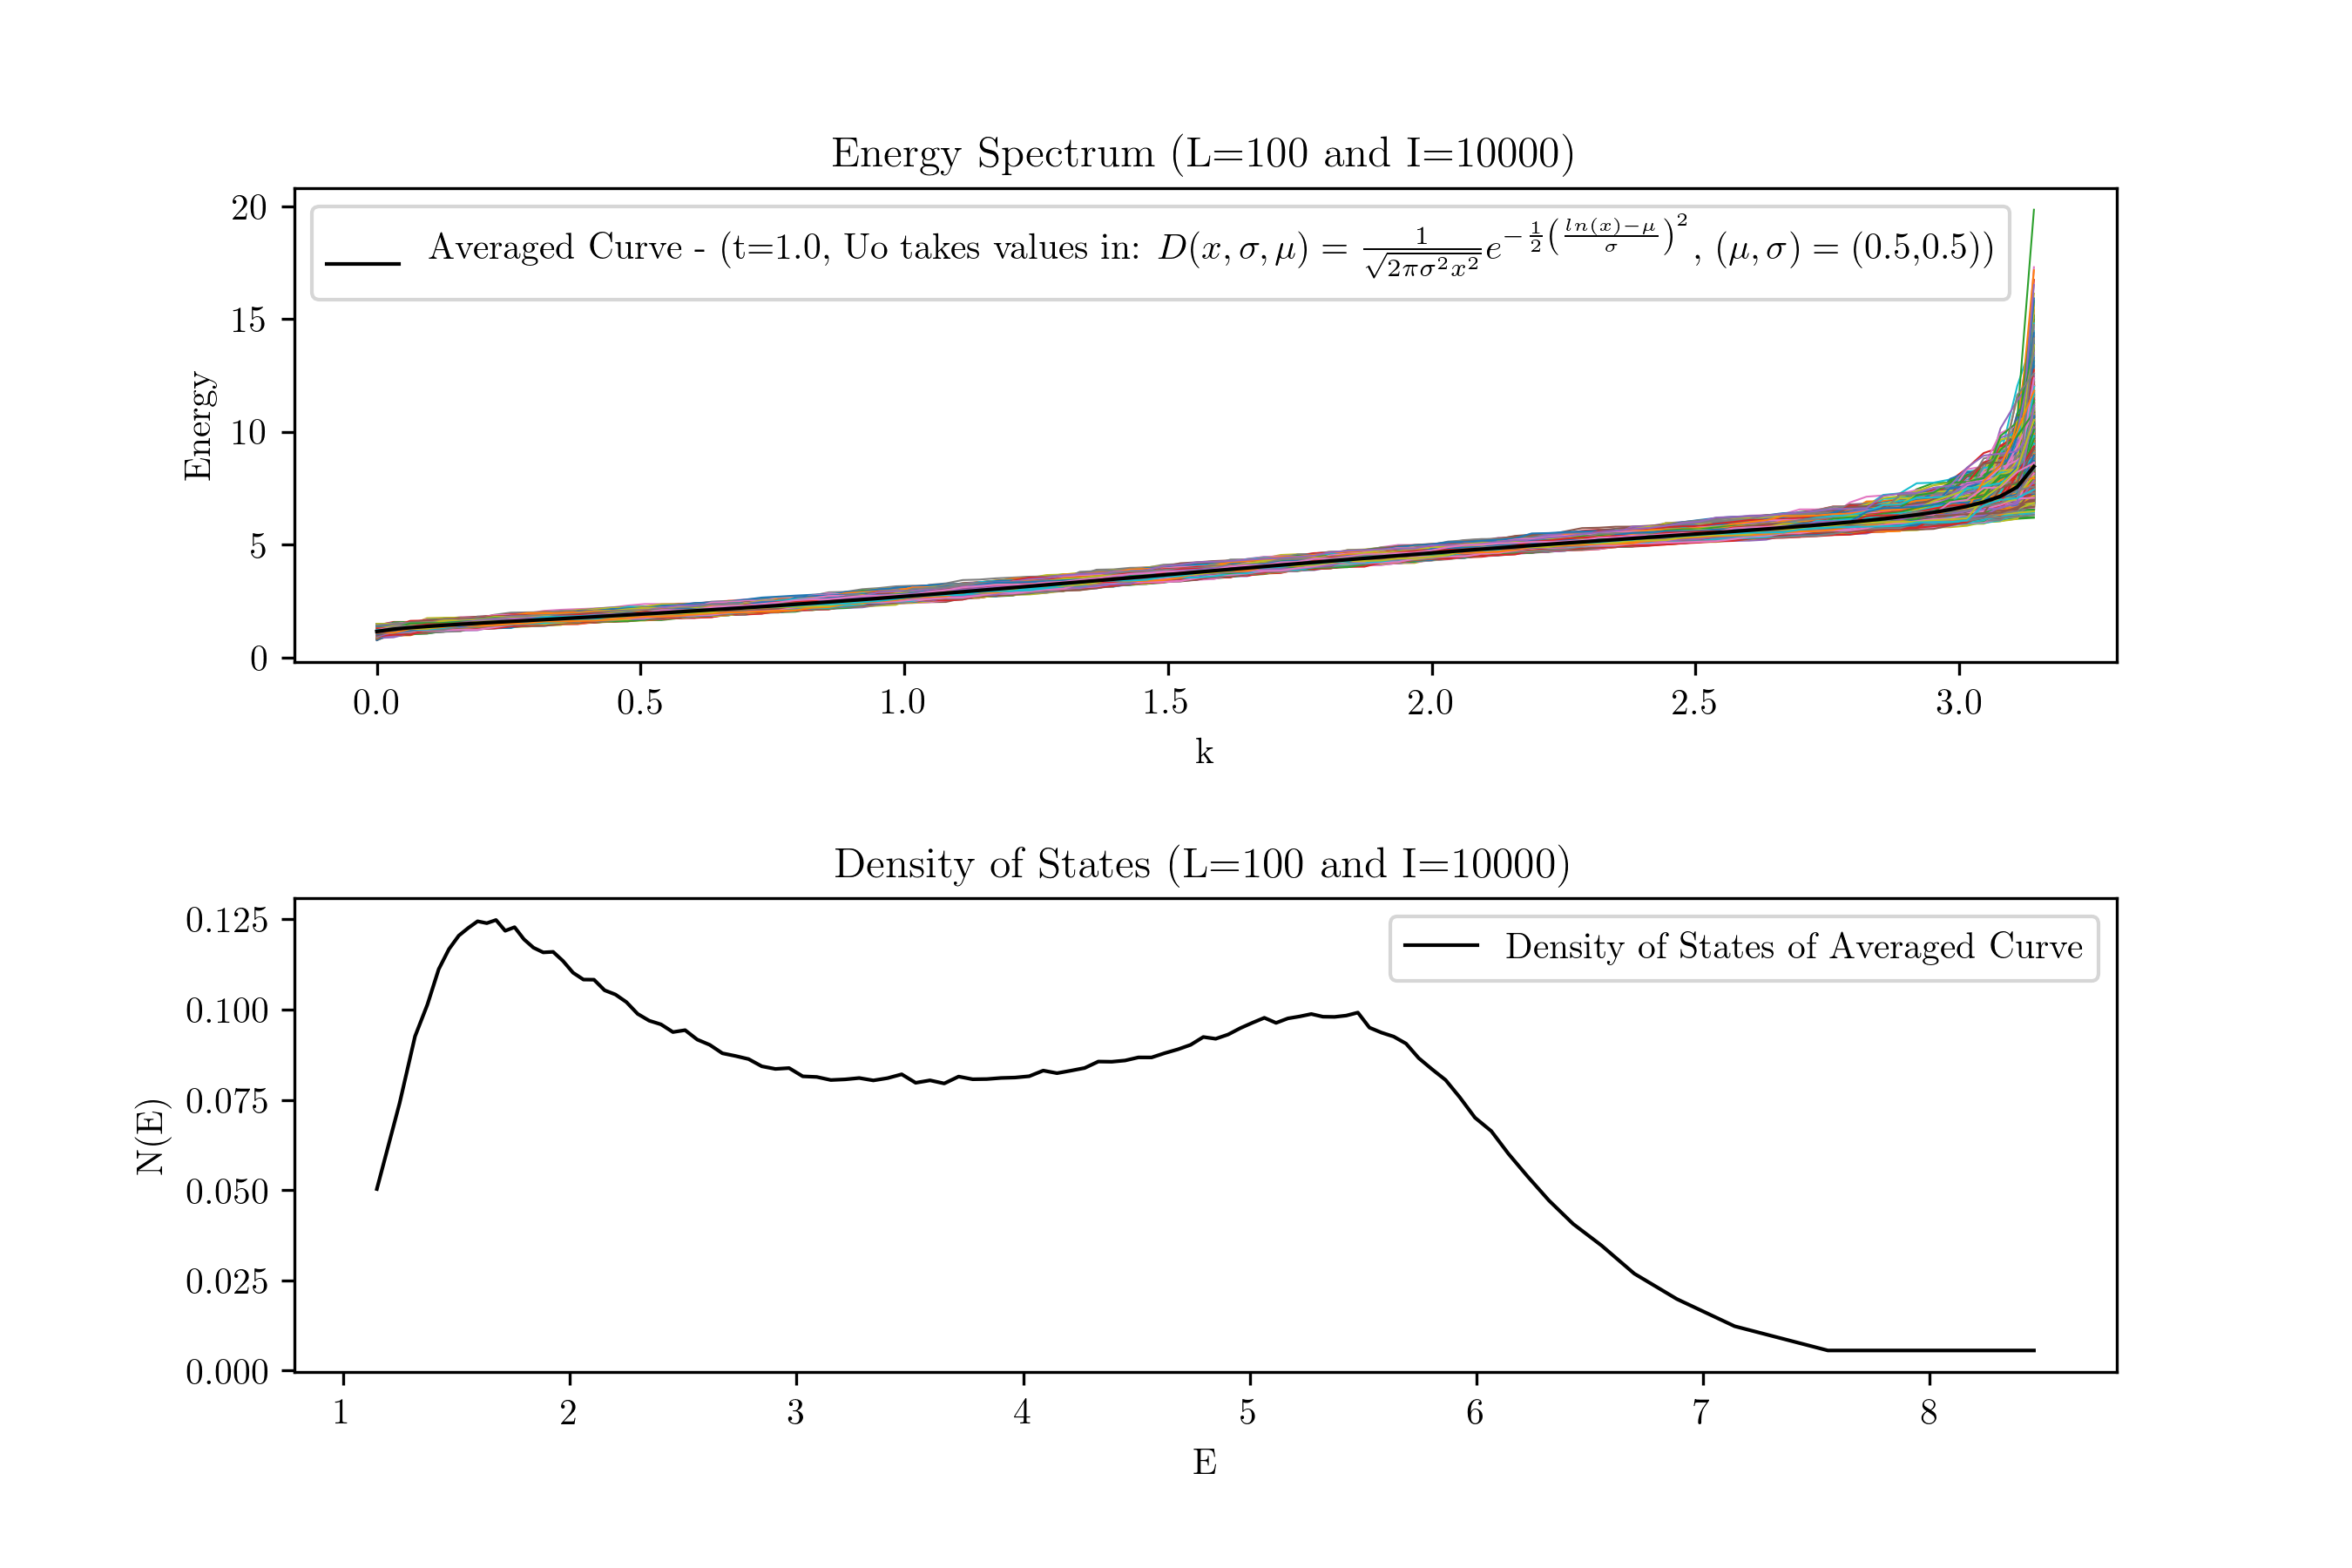
\includegraphics[scale=0.65]{EDOSCRL.png}
                \caption{Energy Spectrum and DoS, on-site potential terms $U_{0}$ take values in a log-normal distribution.}
                \label{f3a}
        \end{subfigure}
        \begin{subfigure}[b]{\textwidth}
        		\centering
                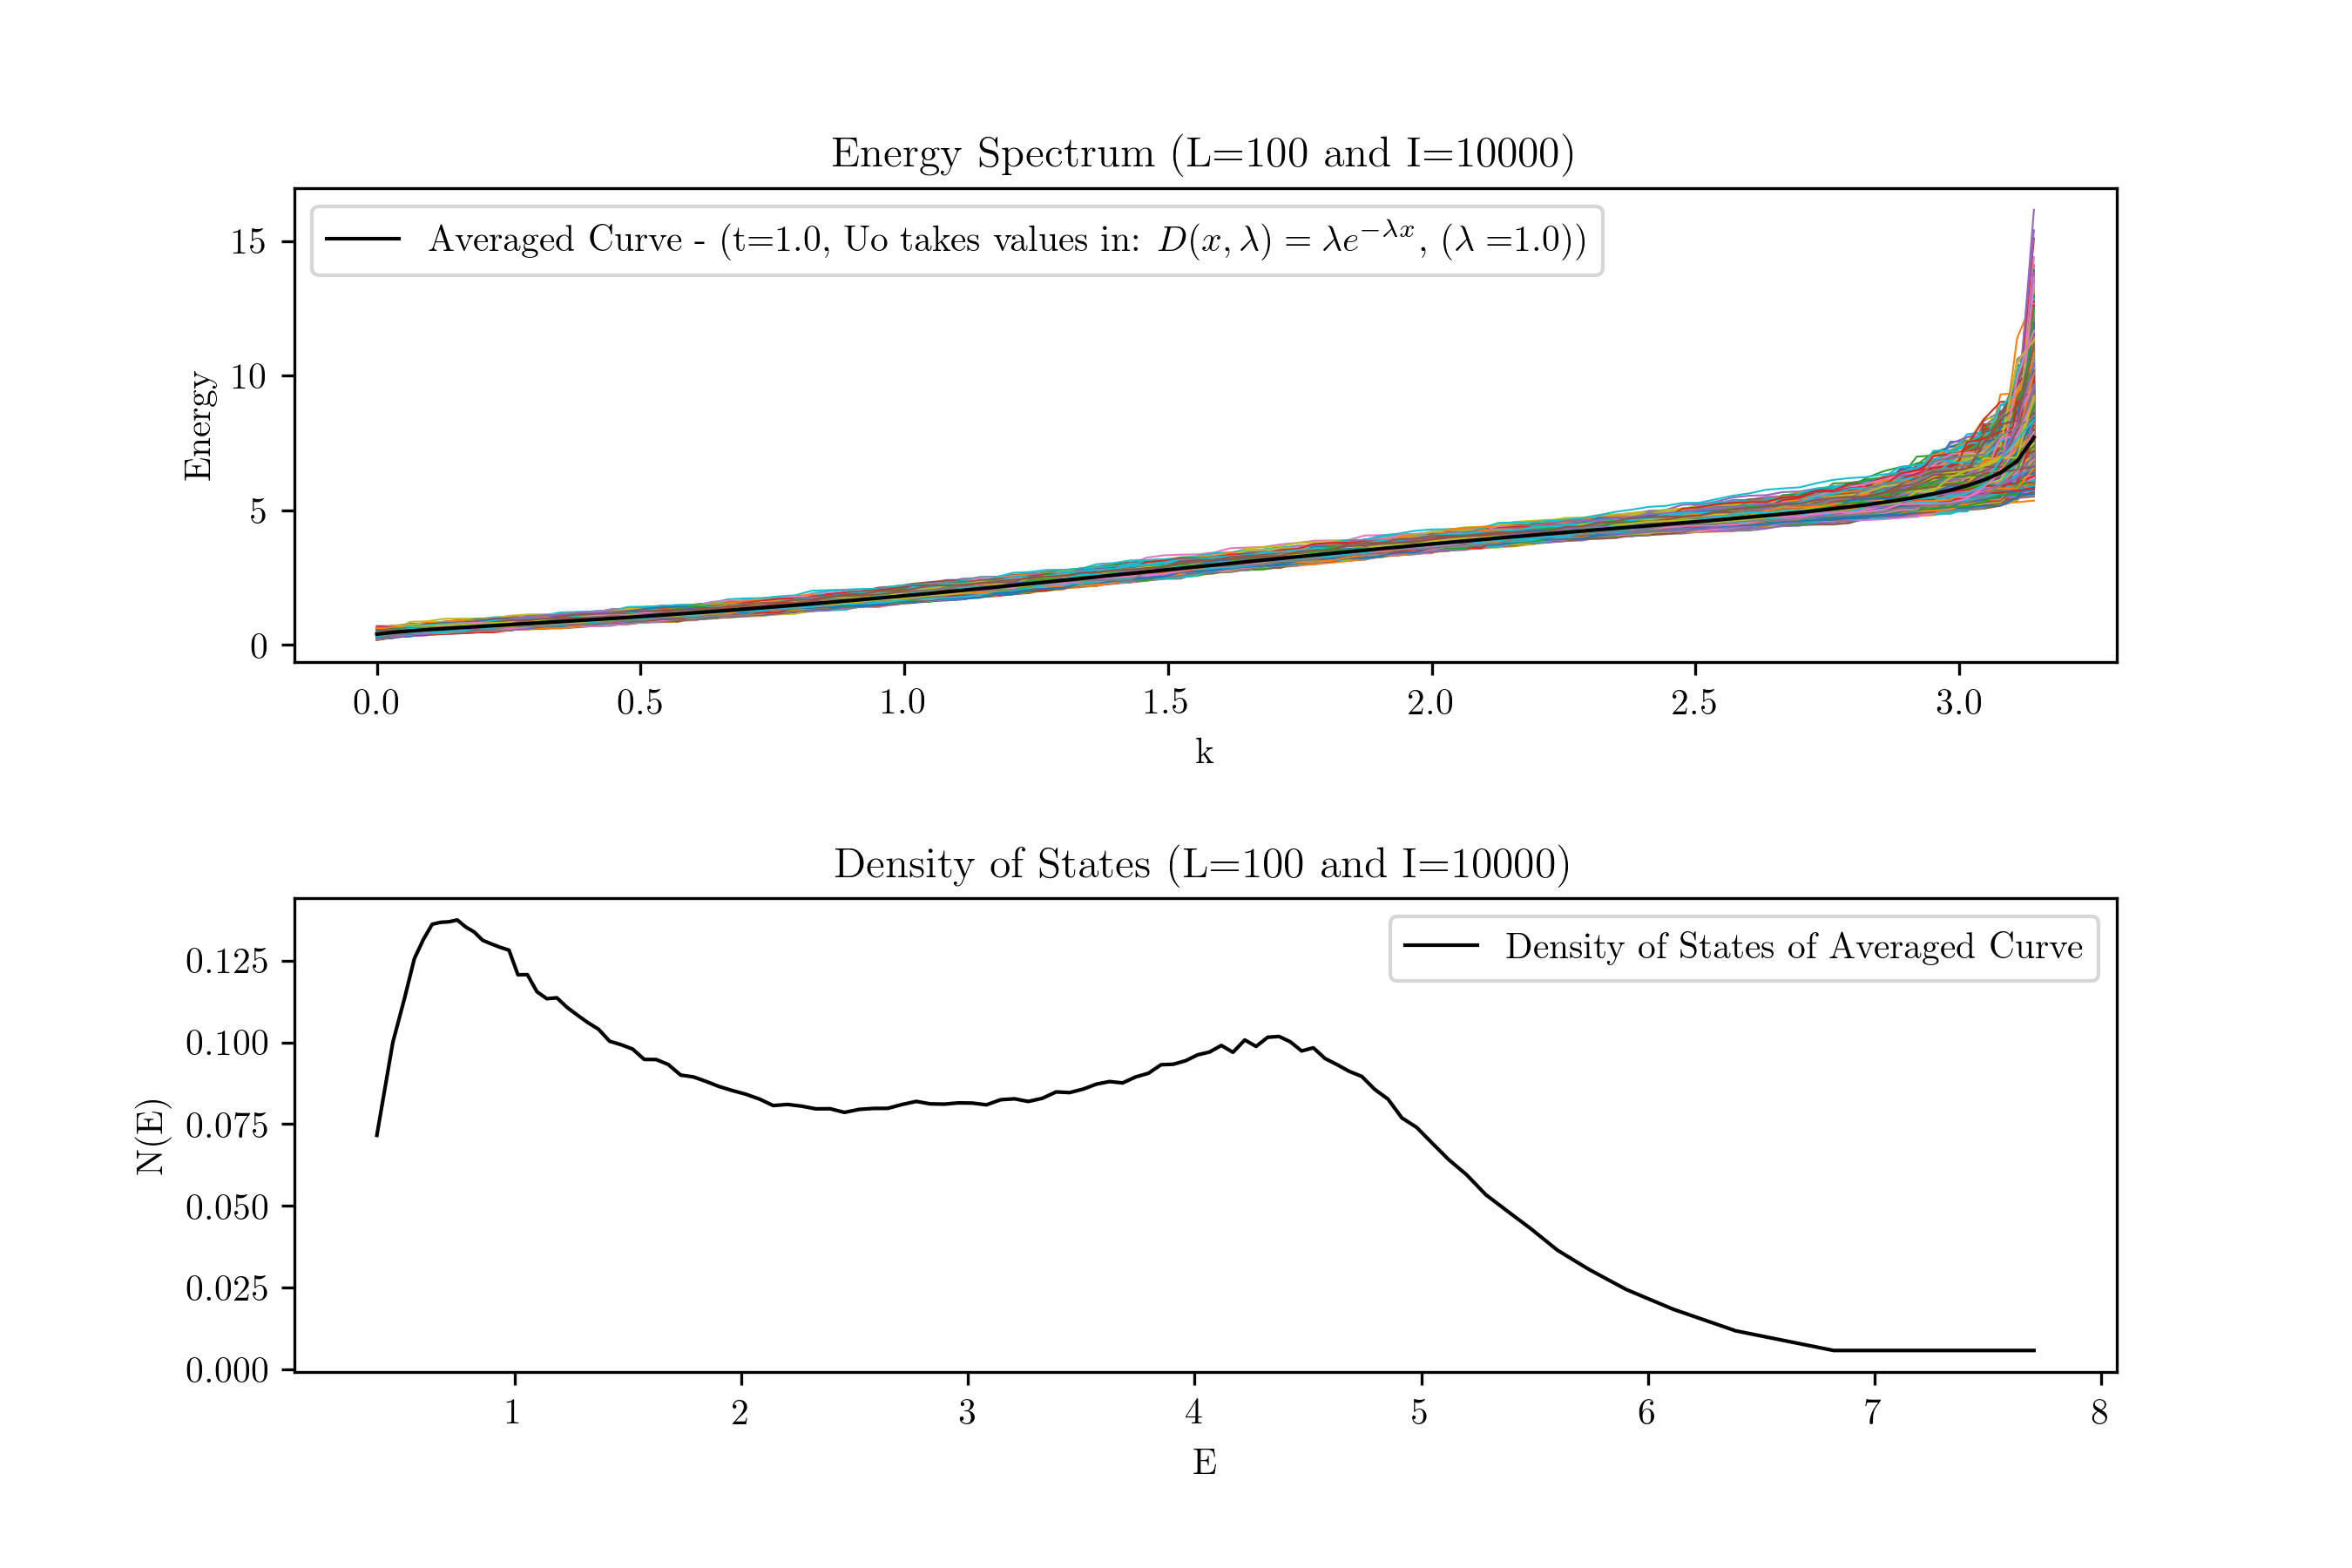
\includegraphics[scale=0.65]{EDOSCRE.png}
                \caption{ Energy Spectrum and DoS, on-site potential terms $U_{0}$ take values in an inverse-exponential distribution.}
                \label{f3b}
        \end{subfigure}
        \caption{Chain of 100 sites and 10000 iterations, on-site potential terms $U_{0}$ take values in: (a) log-normal distribution and (b)  inverse-exponential distribution.}
        \label{f3}
\end{figure}


\begin{figure}[ht]
		\centering
        \begin{subfigure}[a]{\textwidth}
        		\centering
                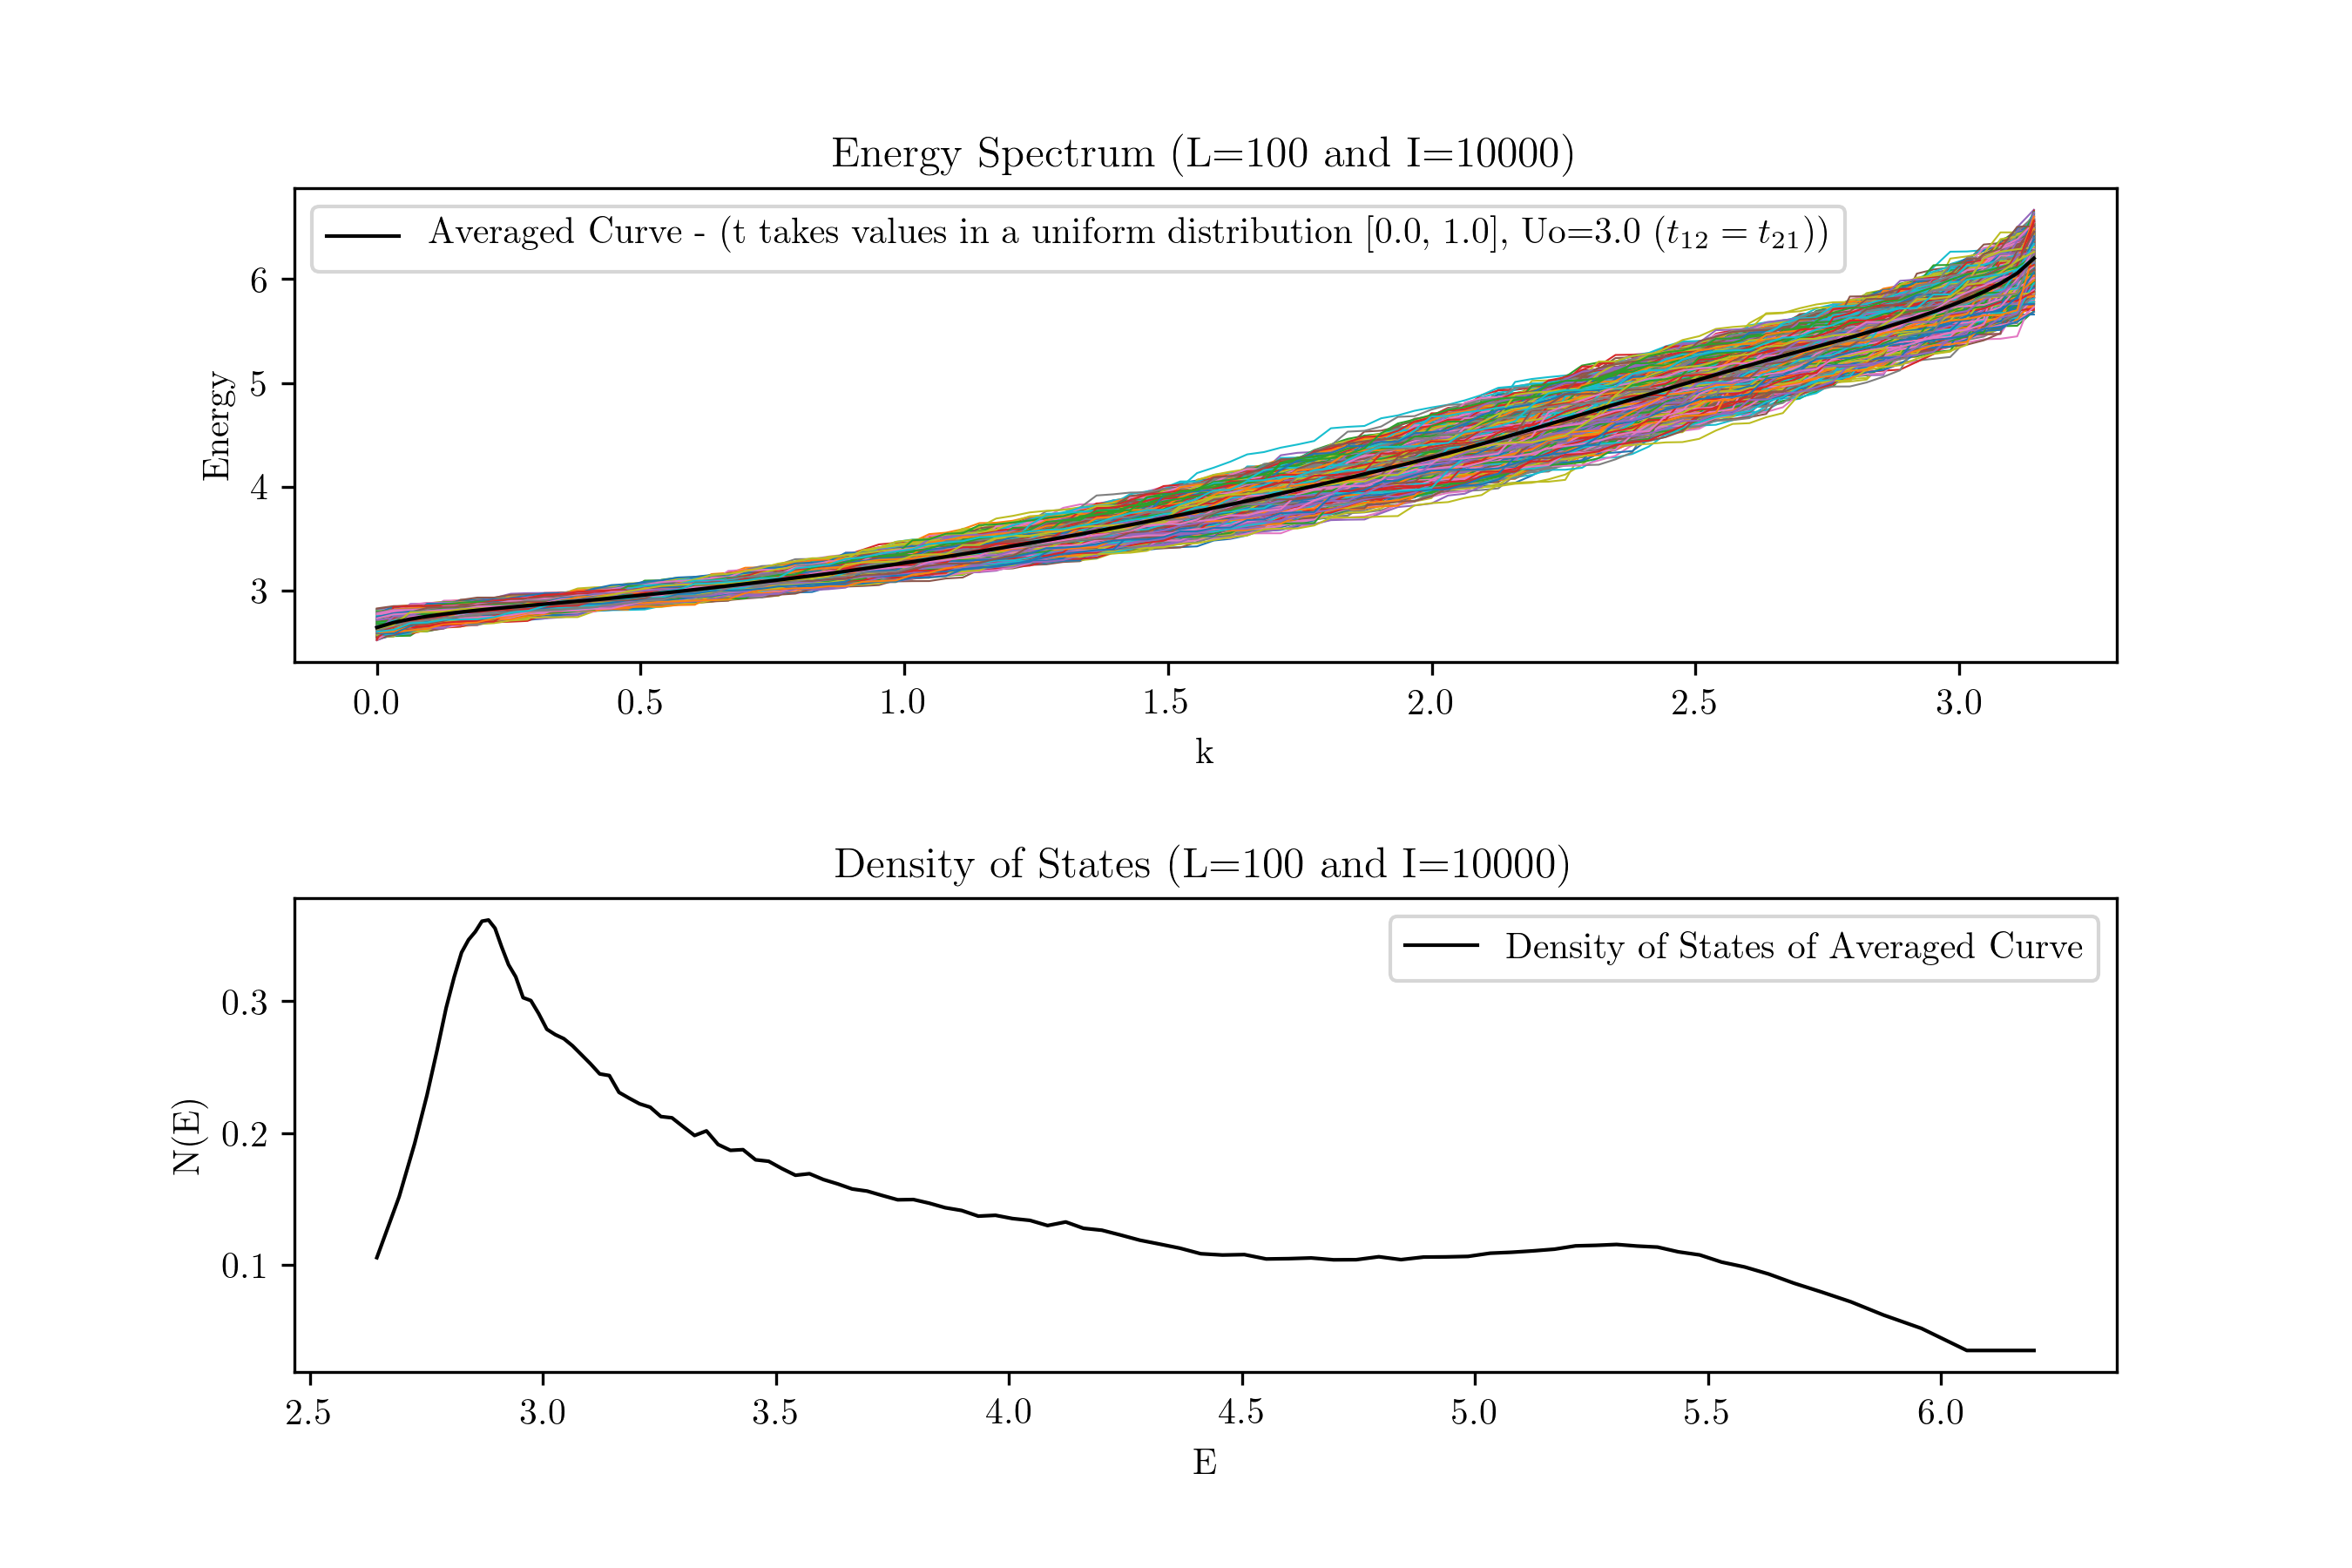
\includegraphics[scale=0.65]{EDOSRoCU.png}
                \caption{Energy Spectrum and DoS, hopping terms $t$ take values in a uniform distribution.}
                \label{f4a}
        \end{subfigure}
        \begin{subfigure}[b]{\textwidth}
        		\centering
                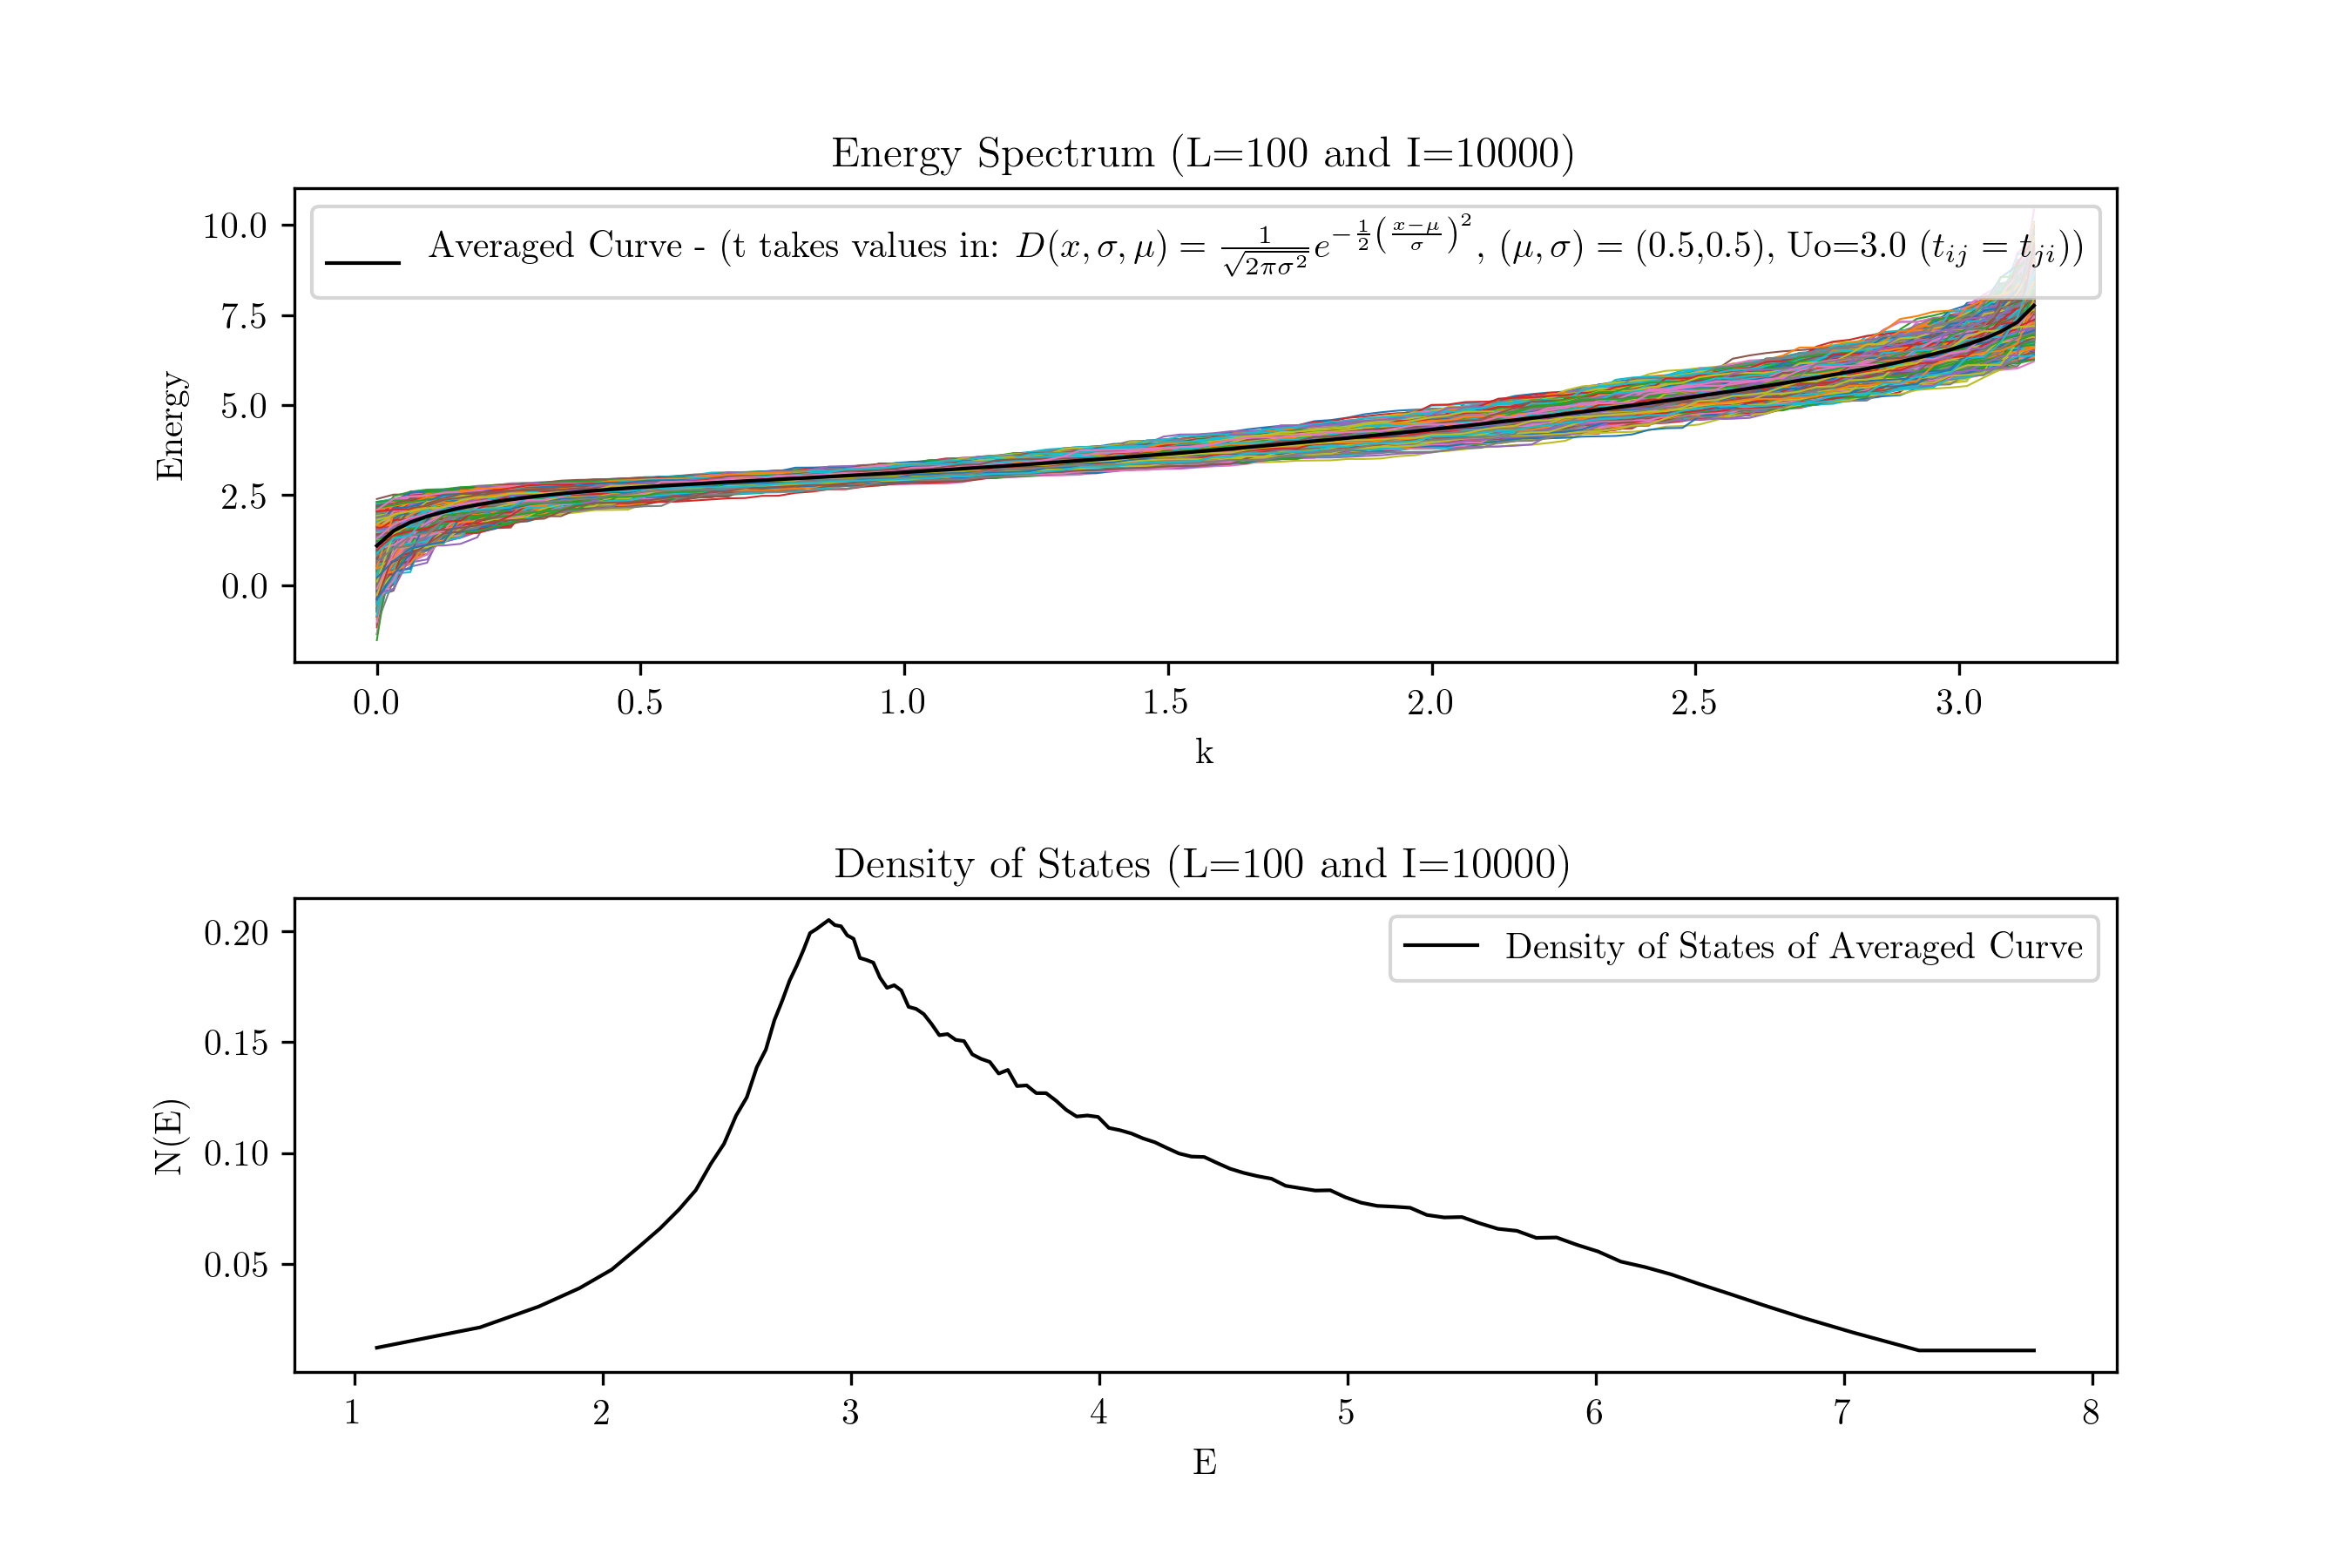
\includegraphics[scale=0.65]{EDOSRoCN.png}
                \caption{ Energy Spectrum and DoS, hopping terms $t$ take values in a normal distribution.}
                \label{f4b}
        \end{subfigure}
        \caption{Chain of 100 sites and 10000 iterations, hopping terms $t$ take values in: (a) uniform distribution and (b)  normal distribution.}
        \label{f4}
\end{figure}

\begin{figure}[ht]
		\centering
        \begin{subfigure}[a]{\textwidth}
        		\centering
                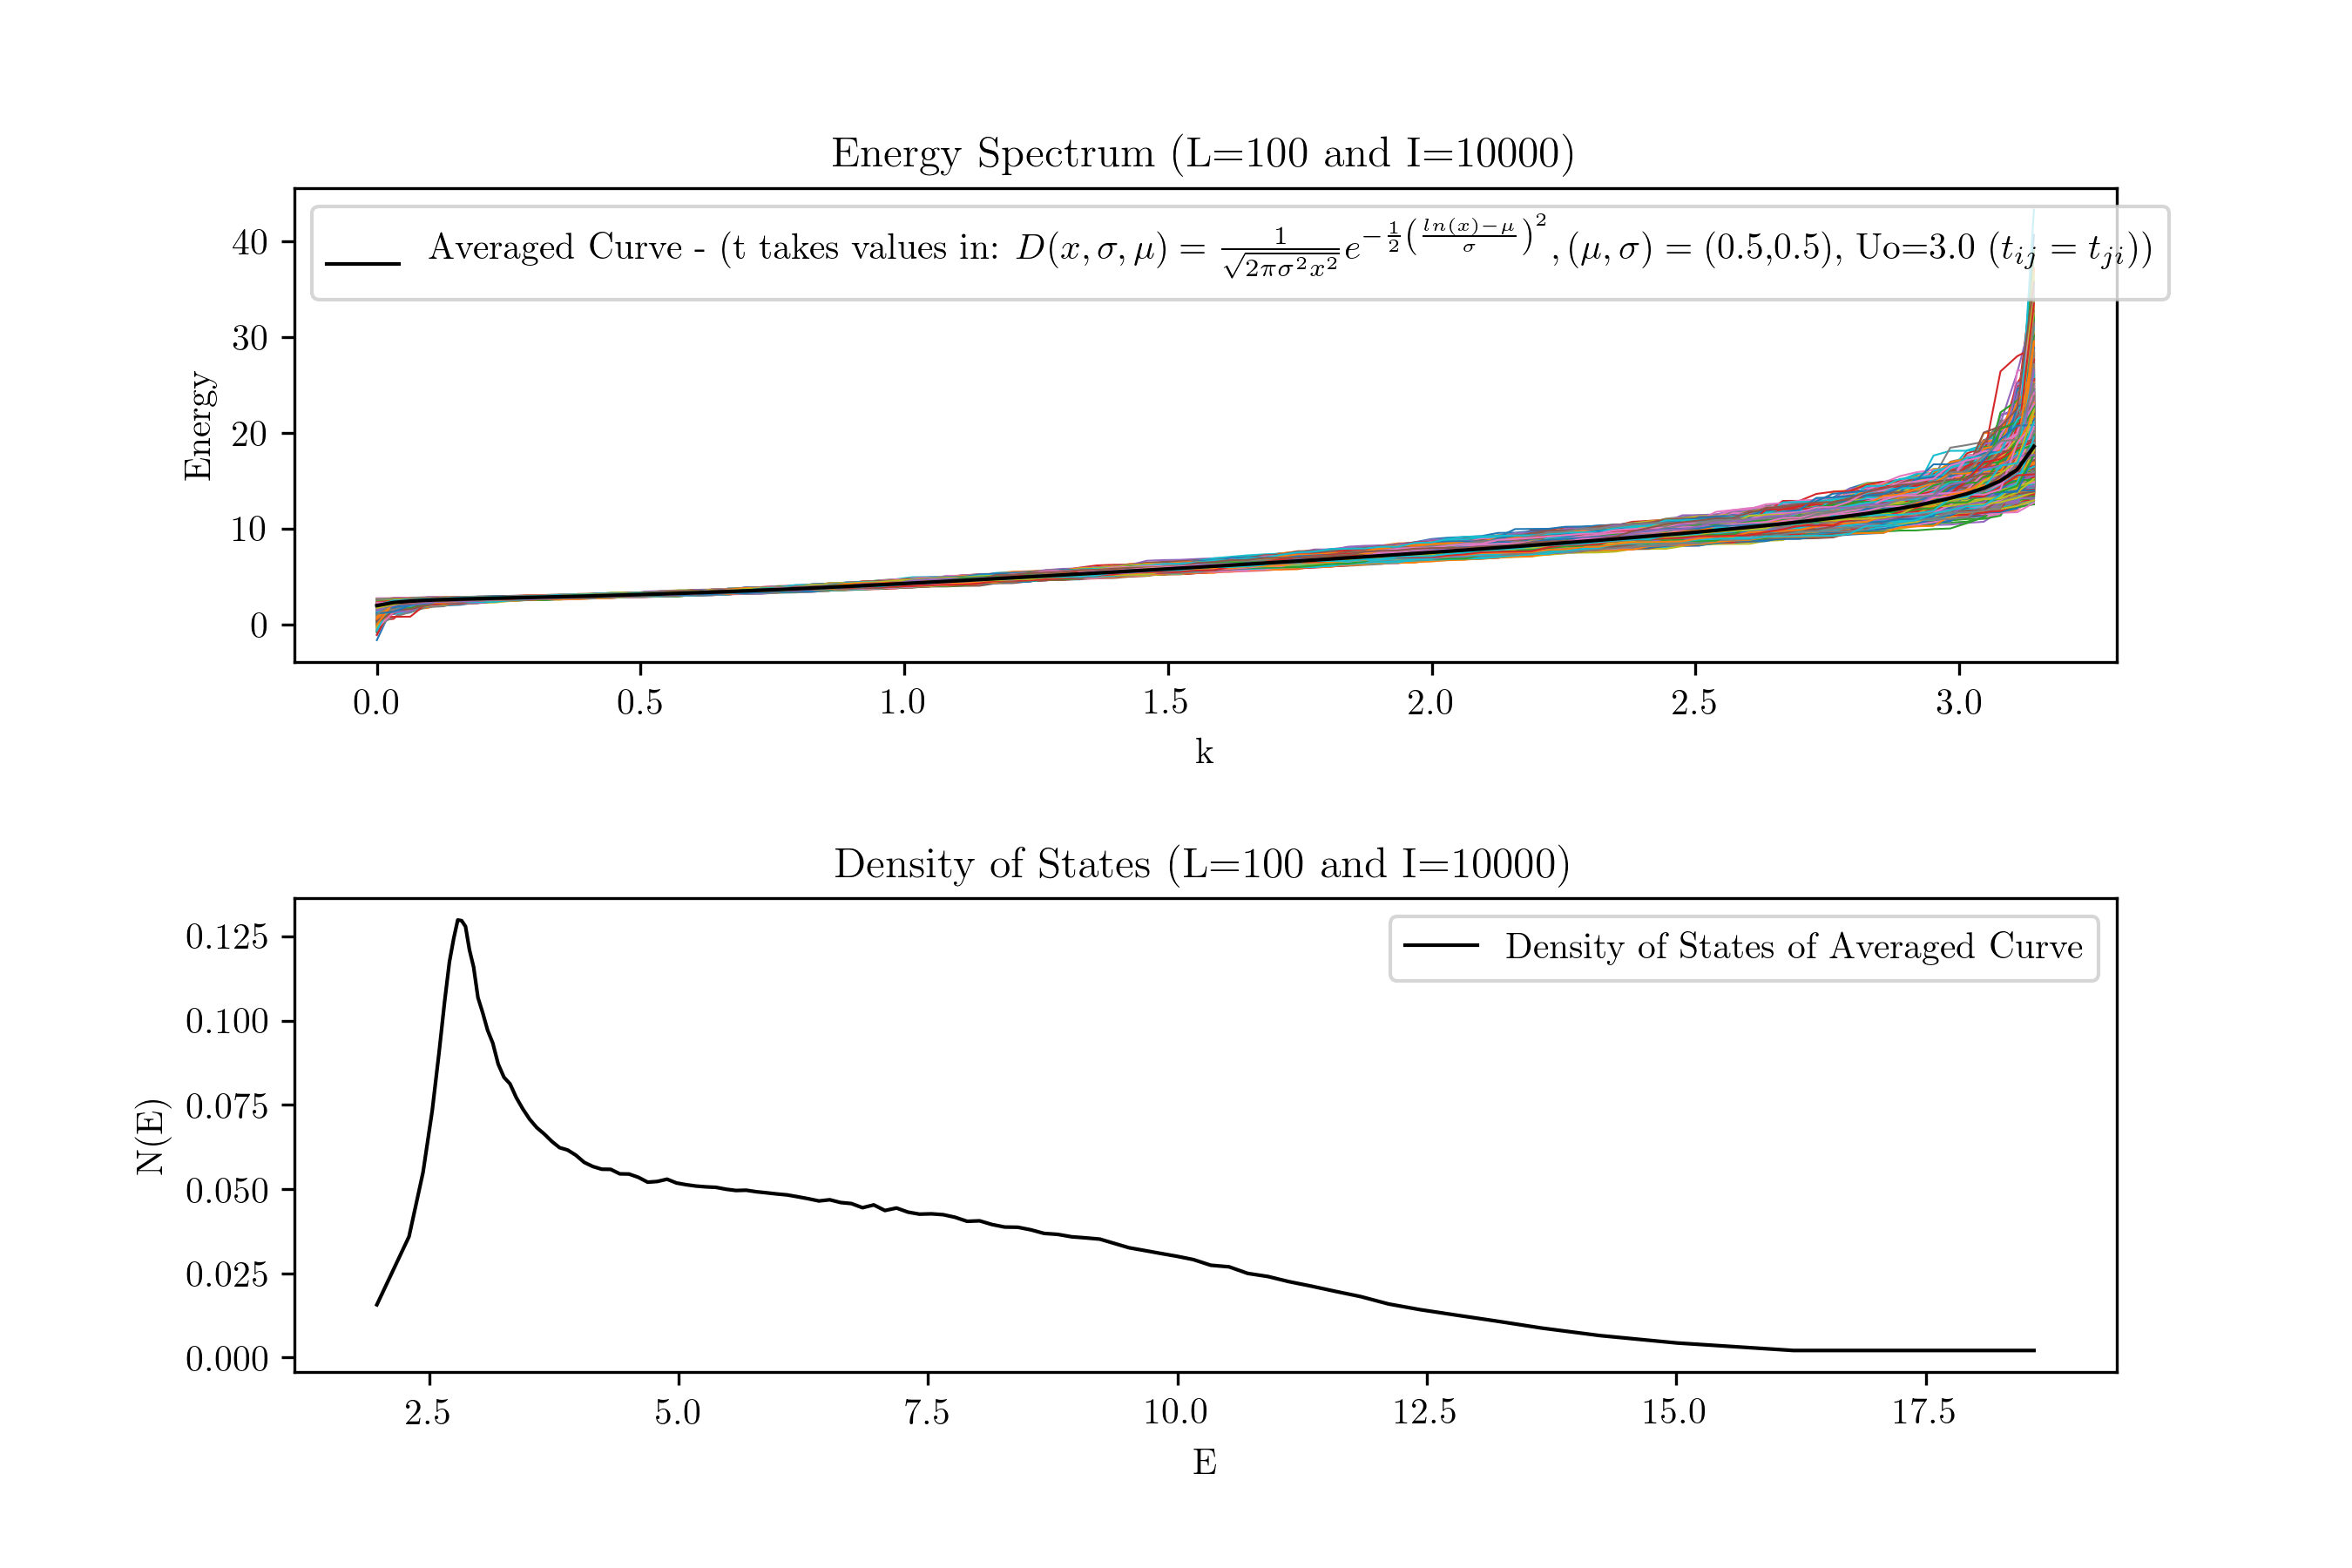
\includegraphics[scale=0.65]{EDOSRoCL.png}
                \caption{Energy Spectrum and DoS, hopping terms $t$ take values in a log-normal distribution.}
                \label{f5a}
        \end{subfigure}
        \begin{subfigure}[b]{\textwidth}
        		\centering
                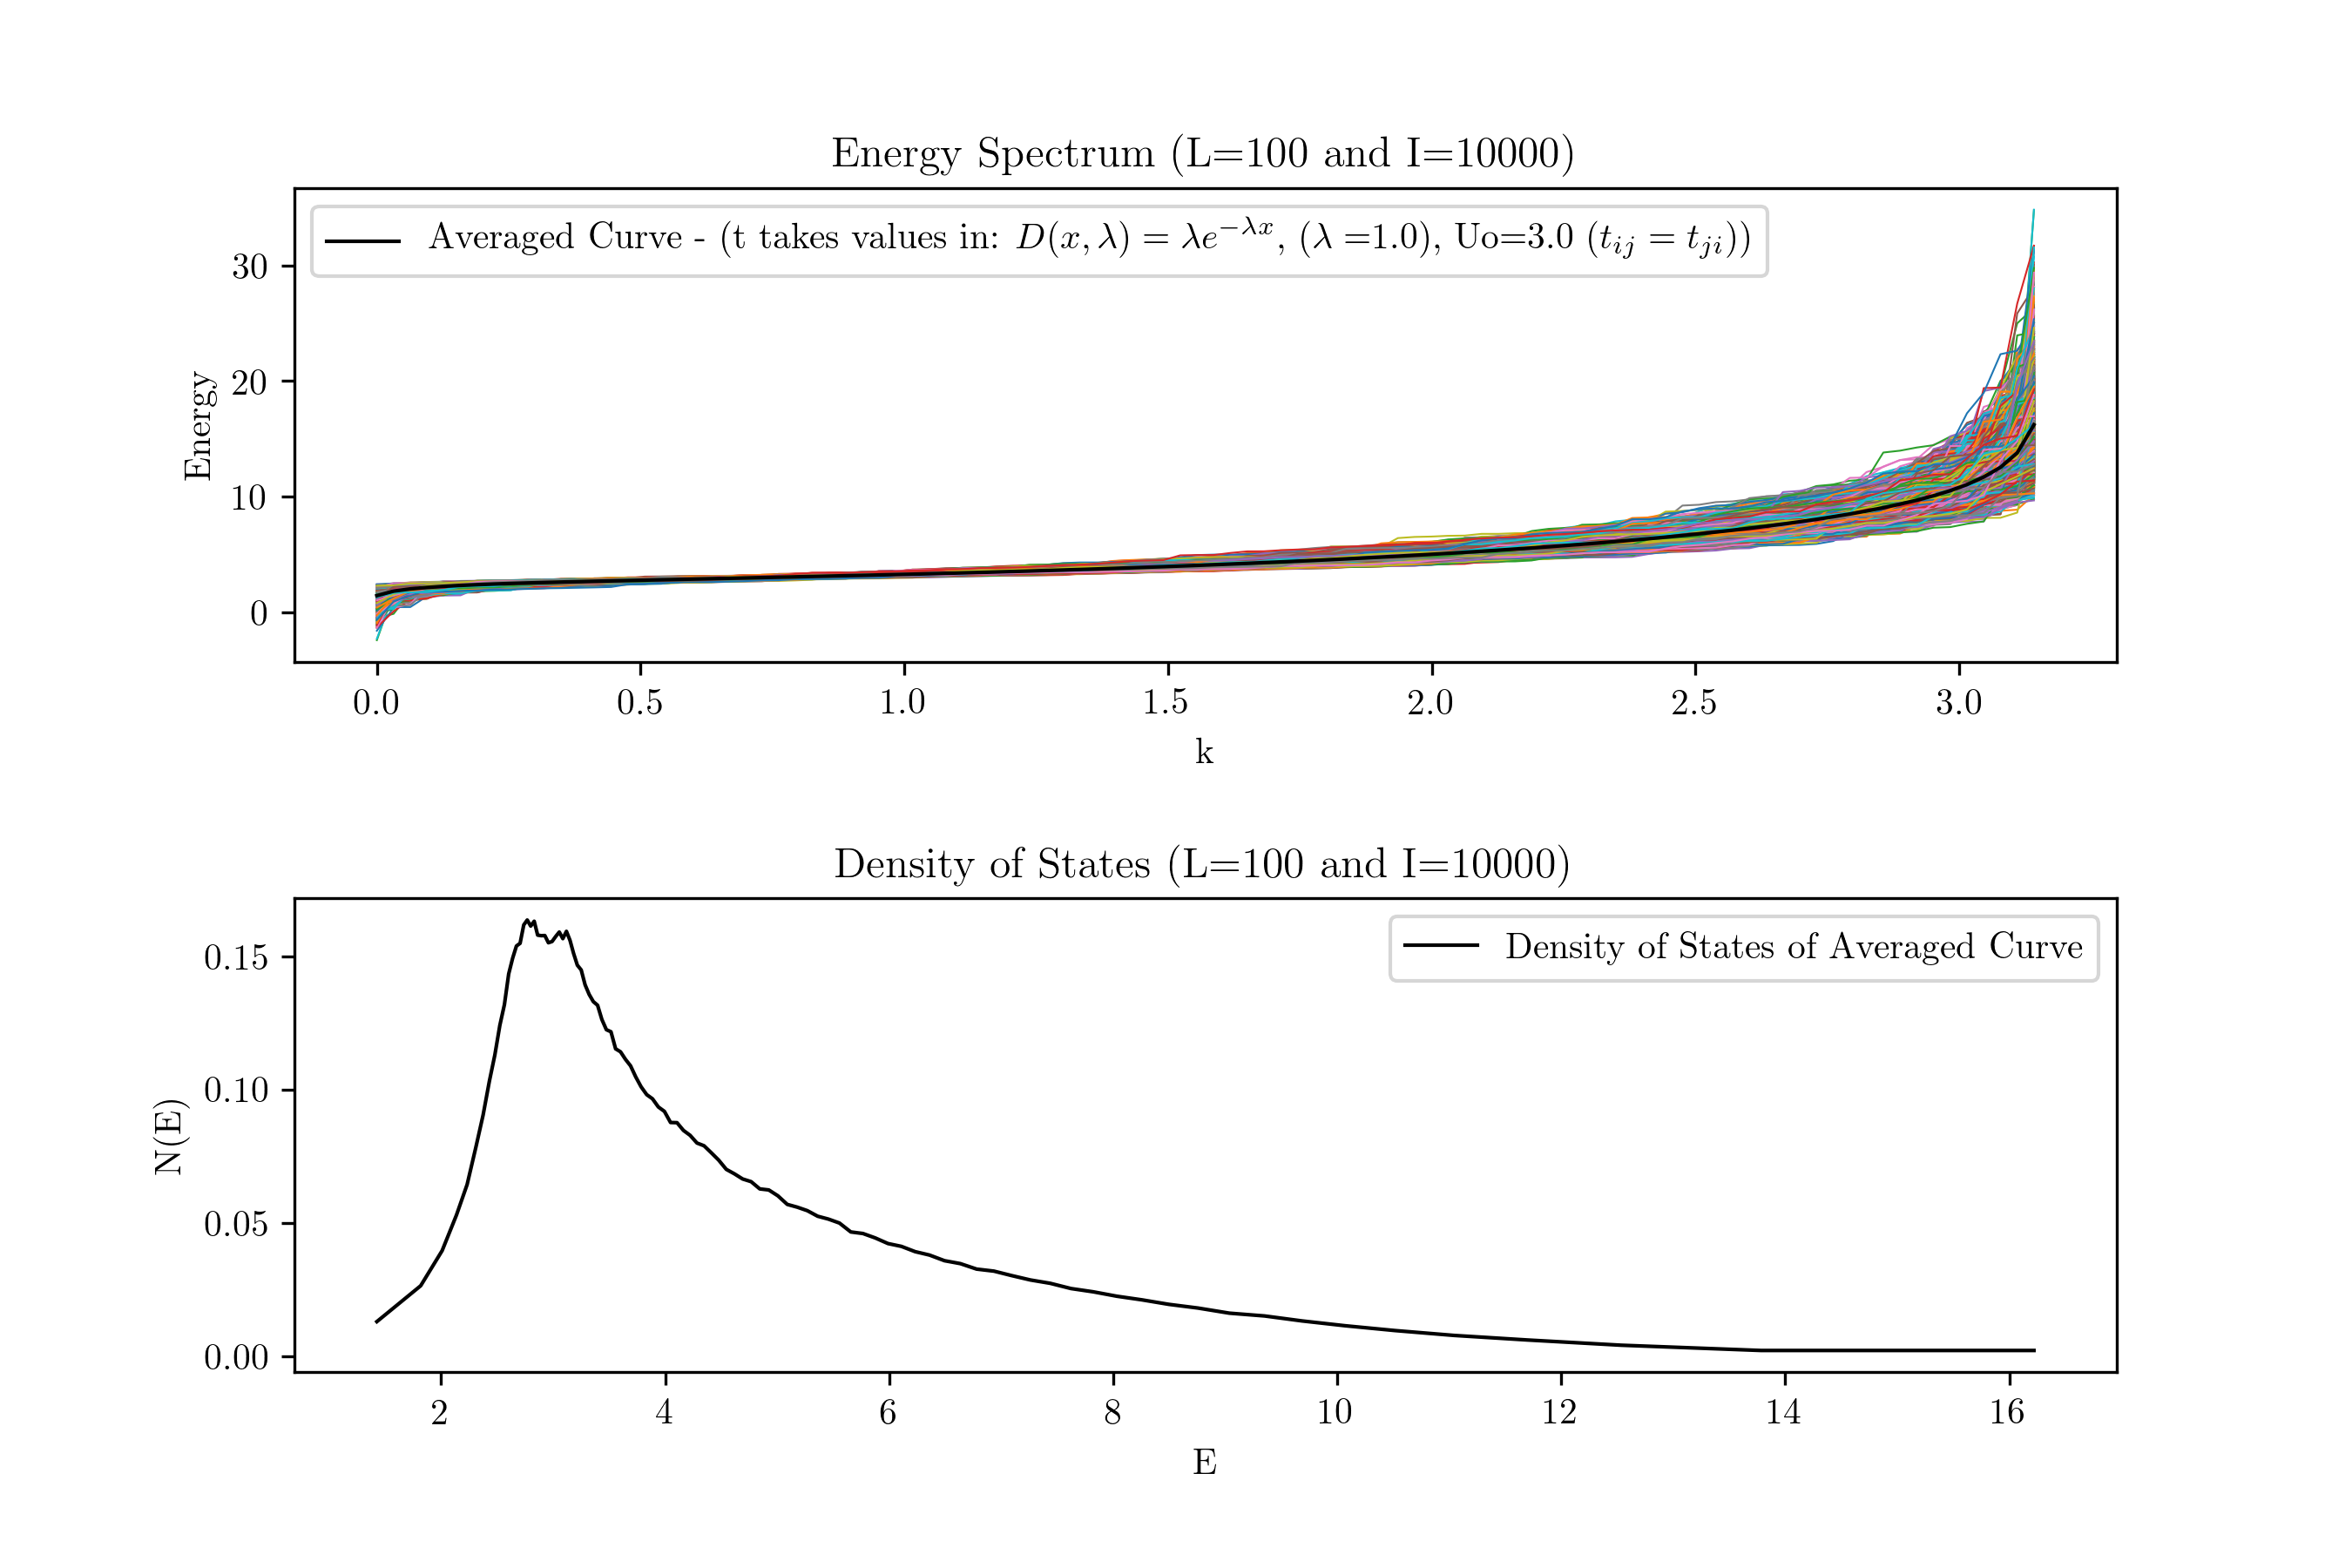
\includegraphics[scale=0.65]{EDOSRoCE.png}
                \caption{ Energy Spectrum and DoS, hopping terms $t$ take values in an inverse-exponential distribution.}
                \label{f5b}
        \end{subfigure}
        \caption{Chain of 100 sites and 10000 iterations, hopping terms $t$ take values in: (a) log-normal distribution and (b)  inverse-exponential distribution.}
        \label{f5}
\end{figure}


\begin{figure}[ht]
		\centering
        \begin{subfigure}[a]{\textwidth}
        		\centering
                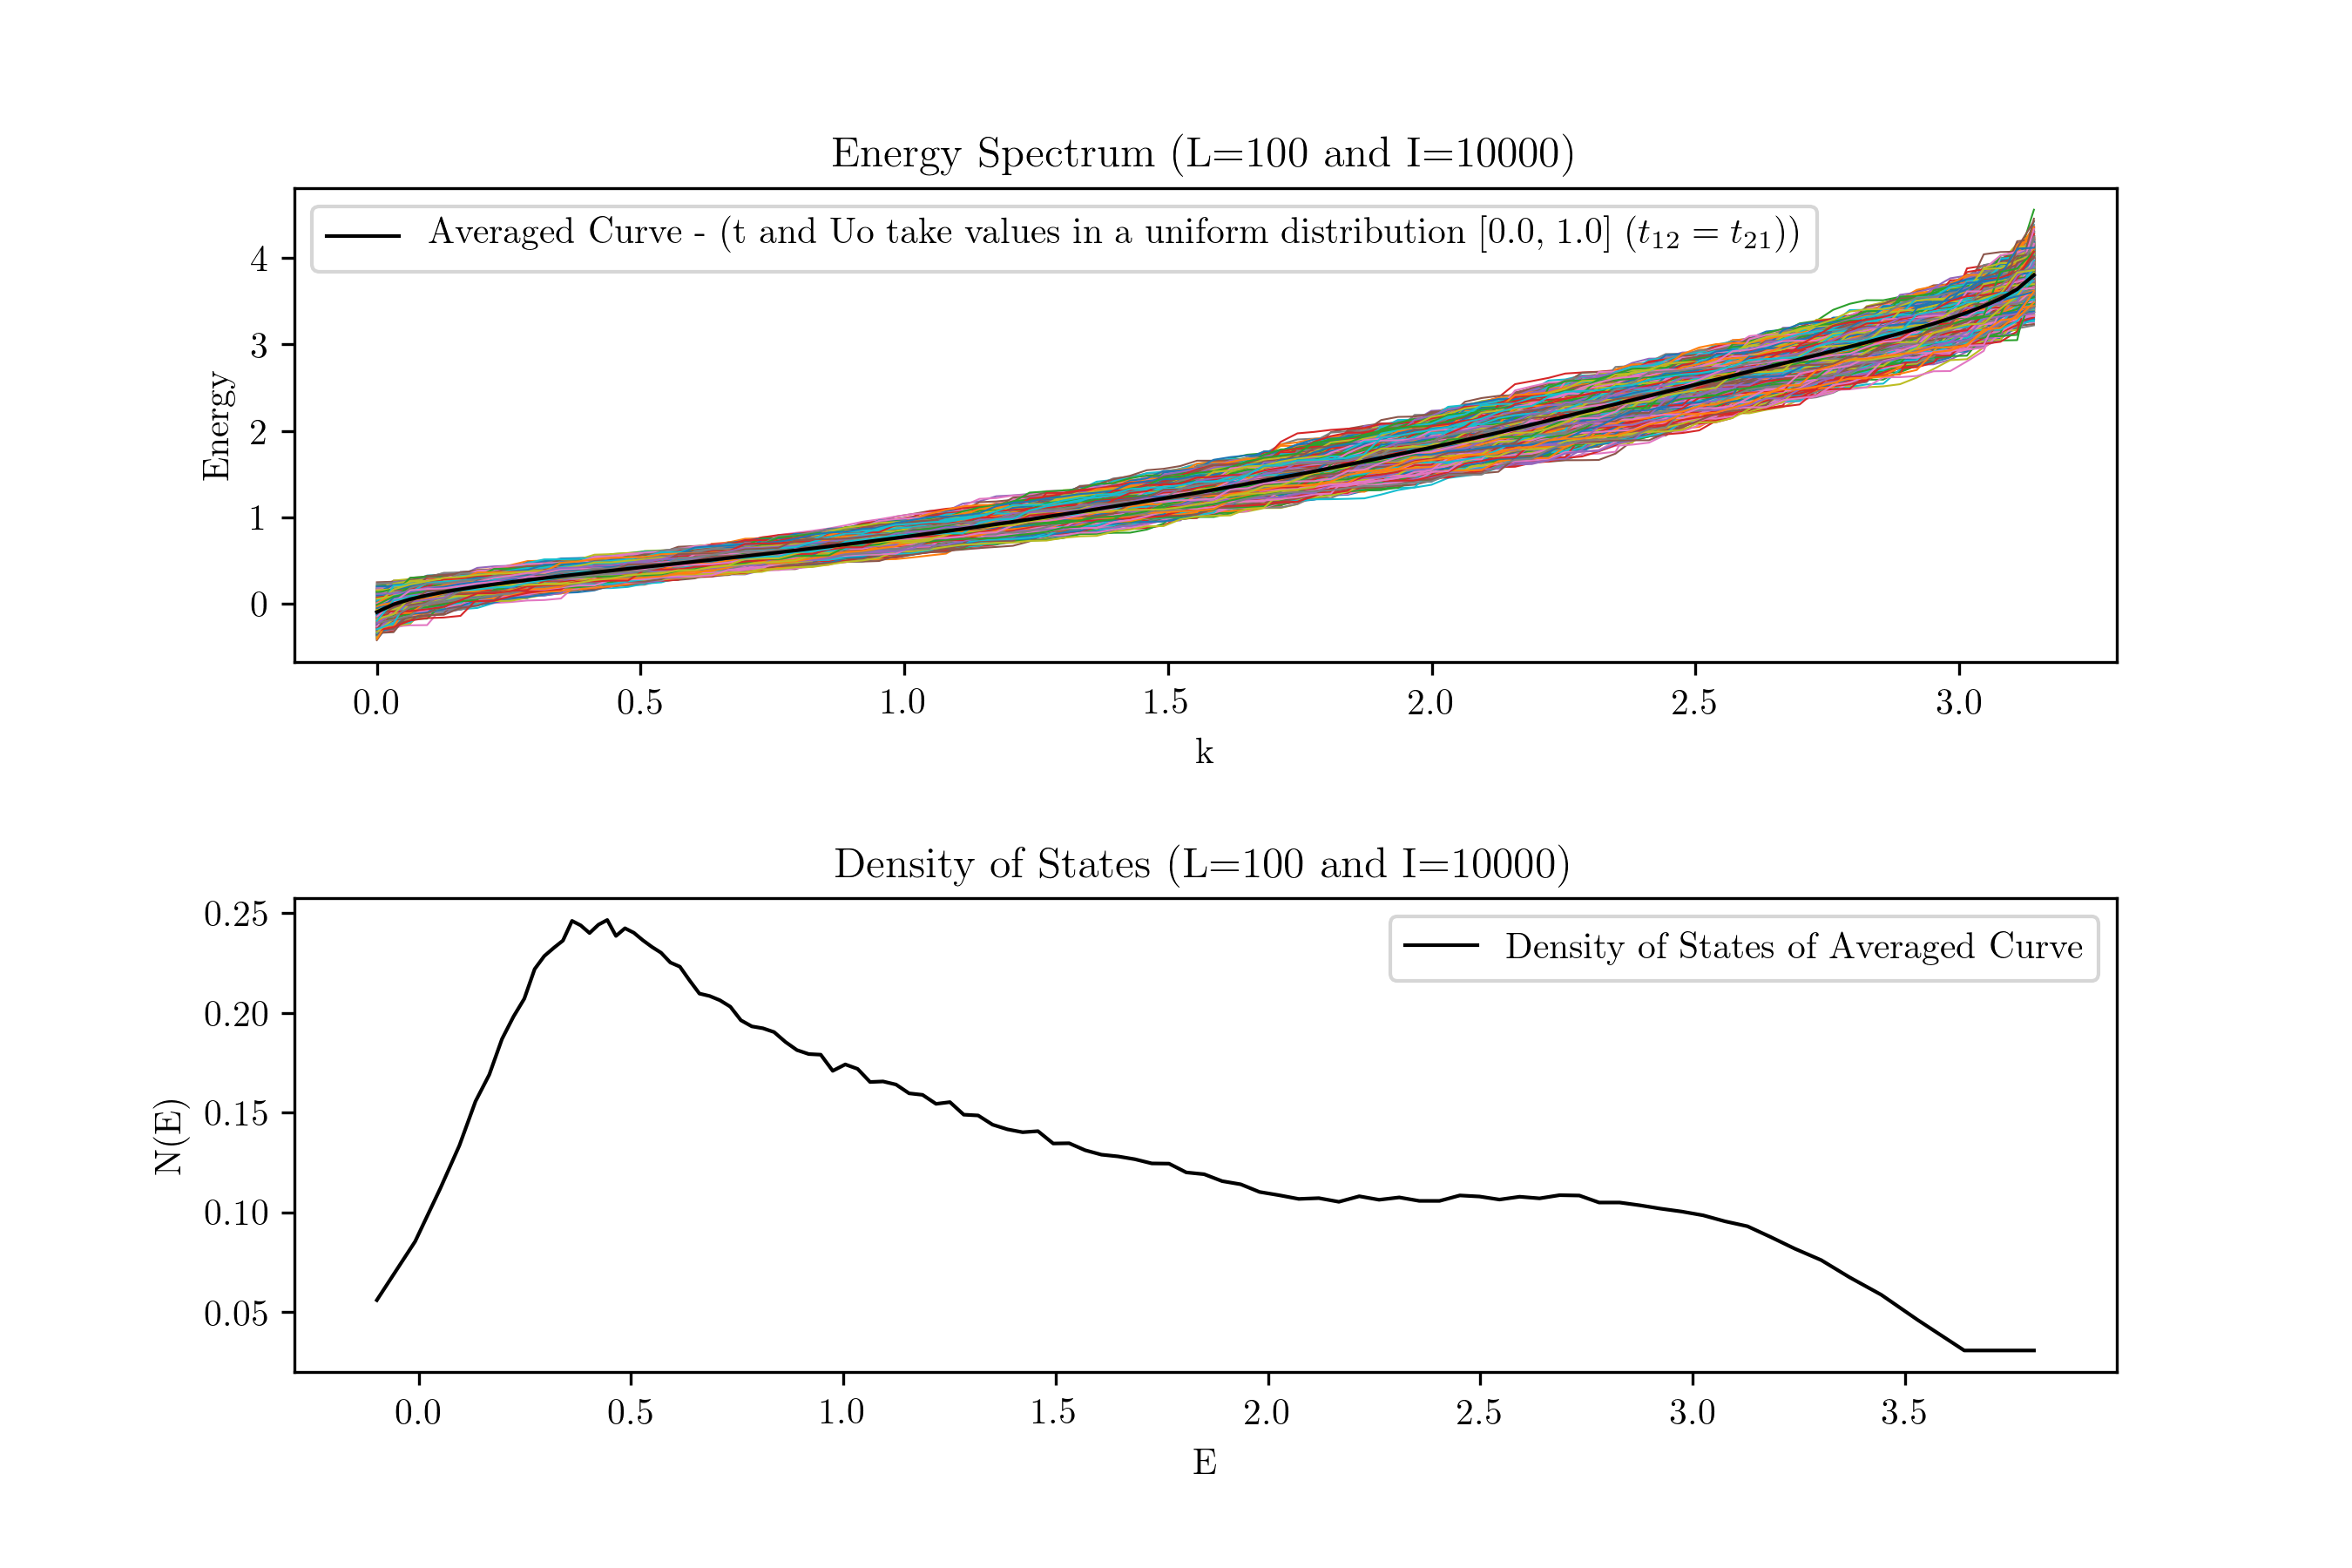
\includegraphics[scale=0.65]{EDOSRoRU.png}
                \caption{Energy Spectrum and DoS, $U_{0}$ and hopping terms $t$ take values in a uniform distribution.}
                \label{f6a}
        \end{subfigure}
        \begin{subfigure}[b]{\textwidth}
        		\centering
                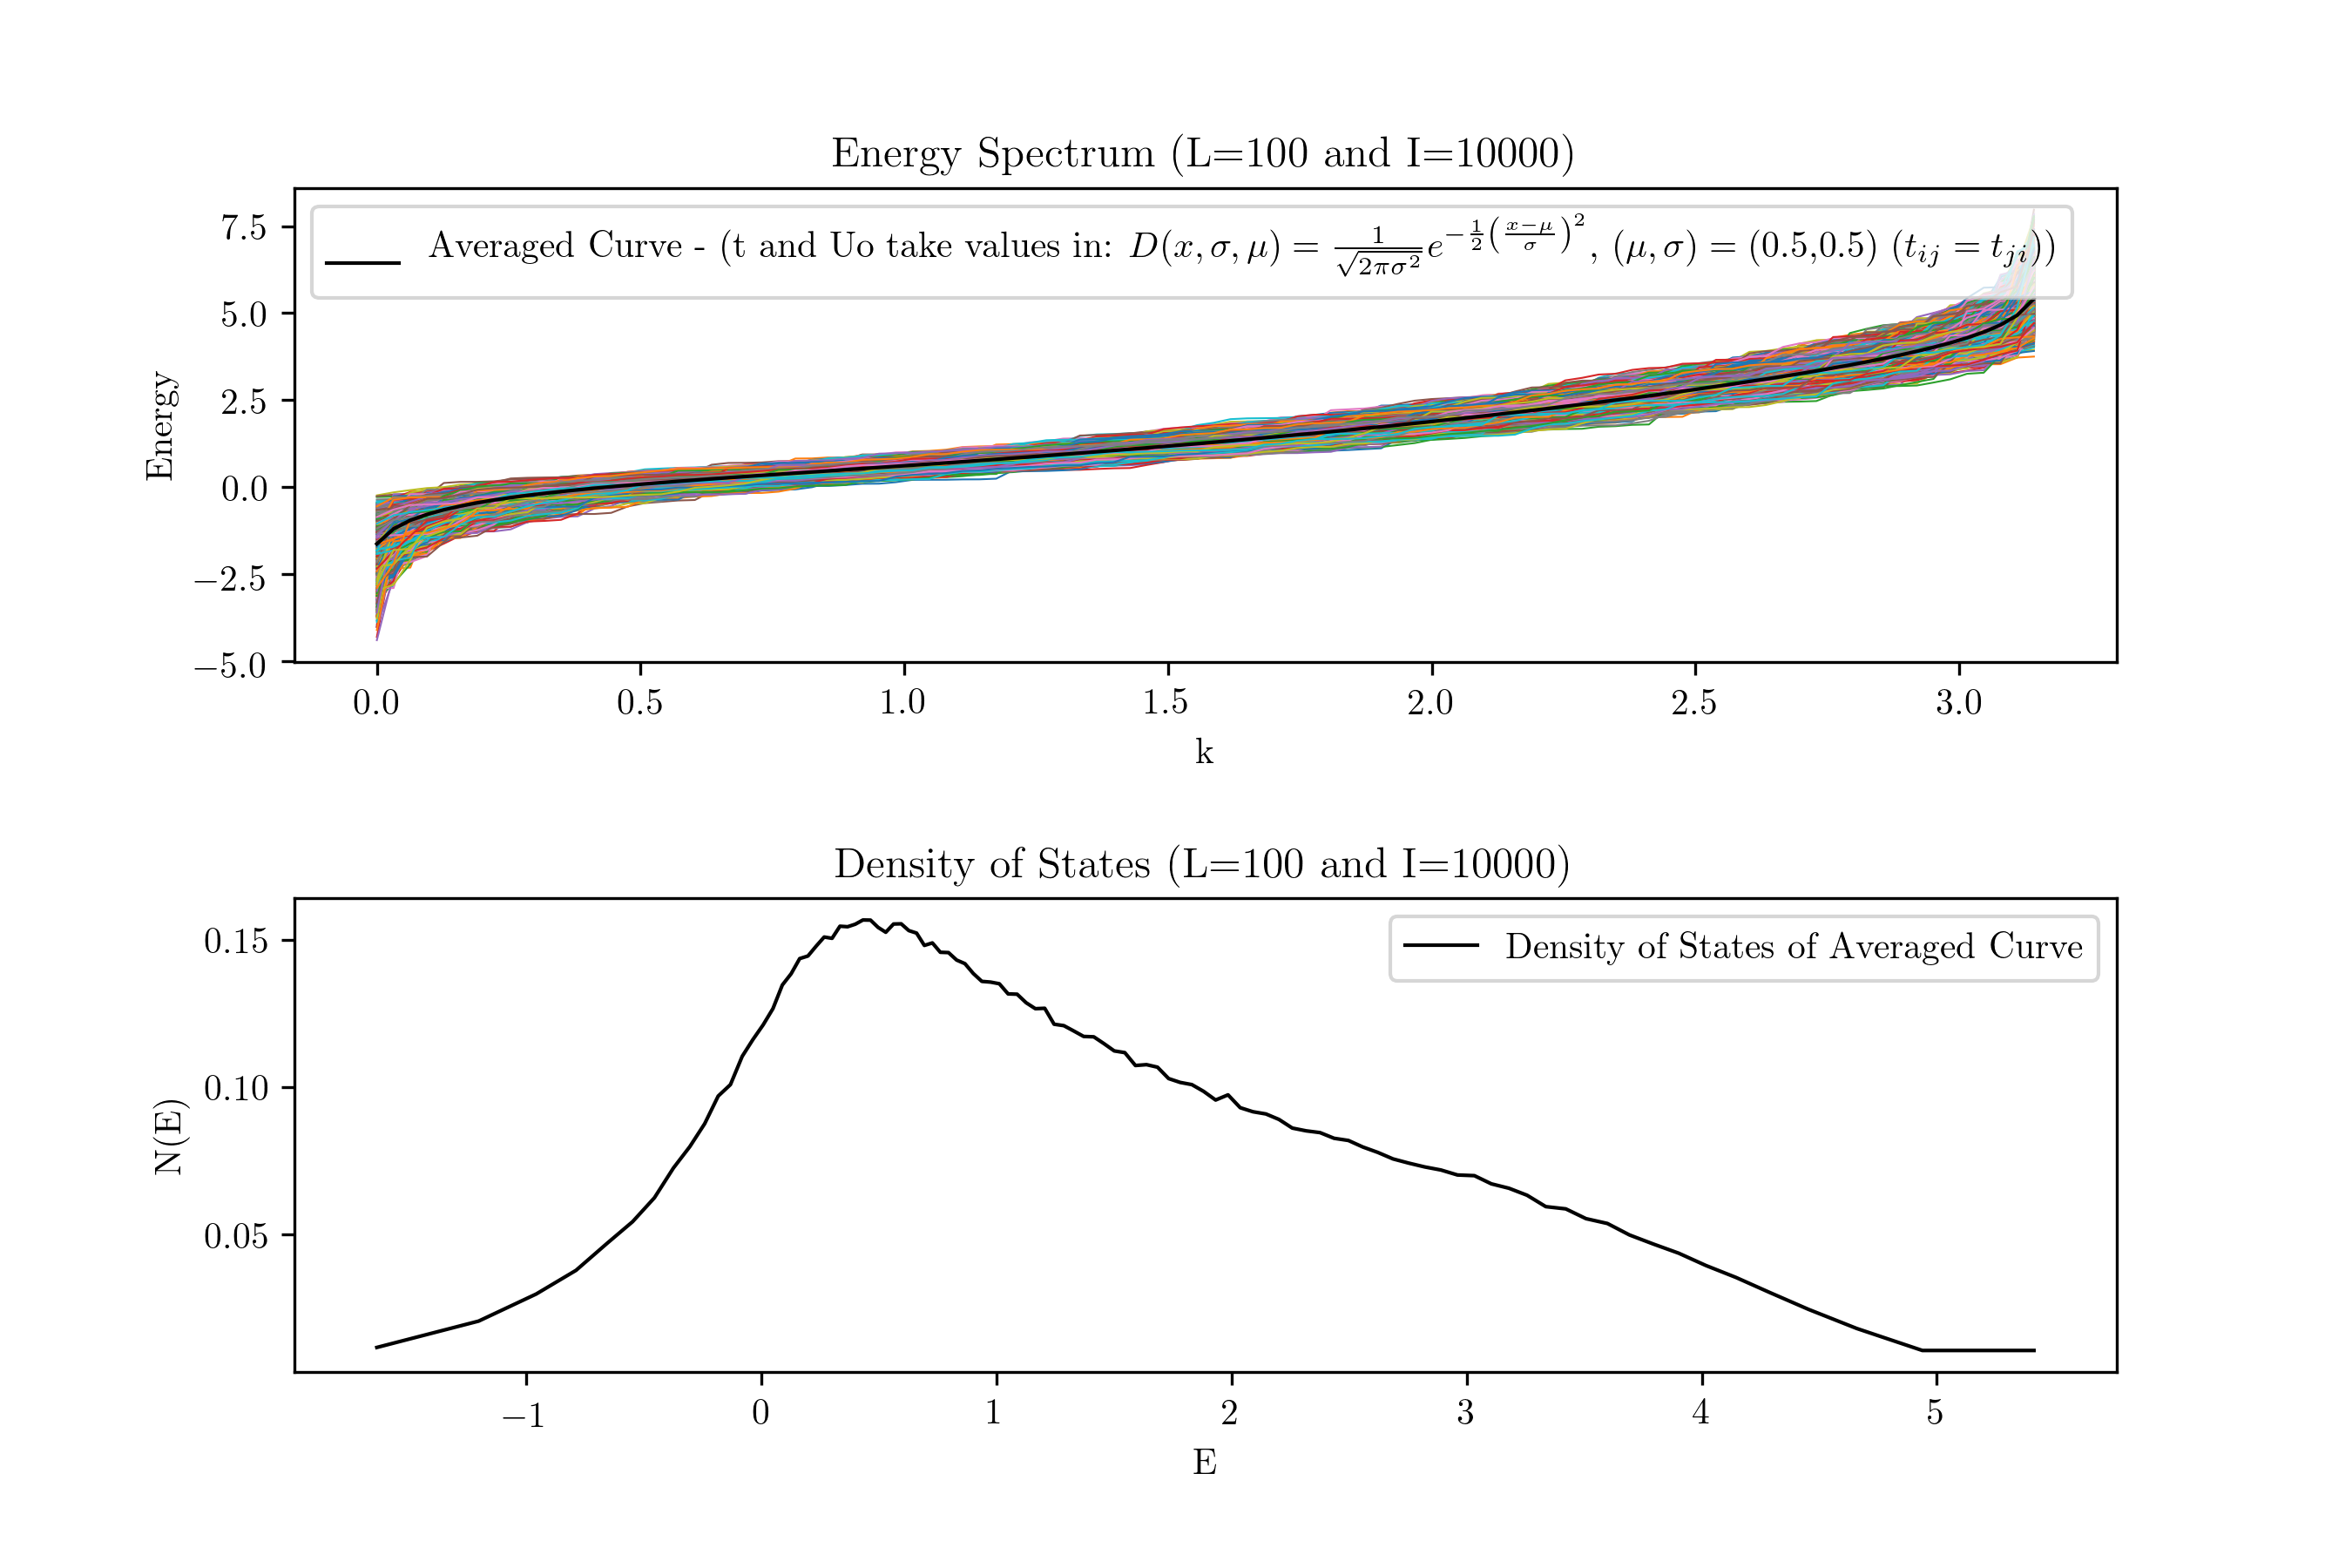
\includegraphics[scale=0.65]{EDOSRoRN.png}
                \caption{ Energy Spectrum and DoS, $U_{0}$ and hopping terms $t$ take values in a normal distribution.}
                \label{f6b}
        \end{subfigure}
        \caption{Chain of 100 sites and 10000 iterations, $U_{0}$ and hopping terms $t$ take values in: (a) uniform distribution and (b)  normal distribution.}
        \label{f6}
\end{figure}



\begin{figure}[ht]
		\centering
        \begin{subfigure}[a]{\textwidth}
        		\centering
                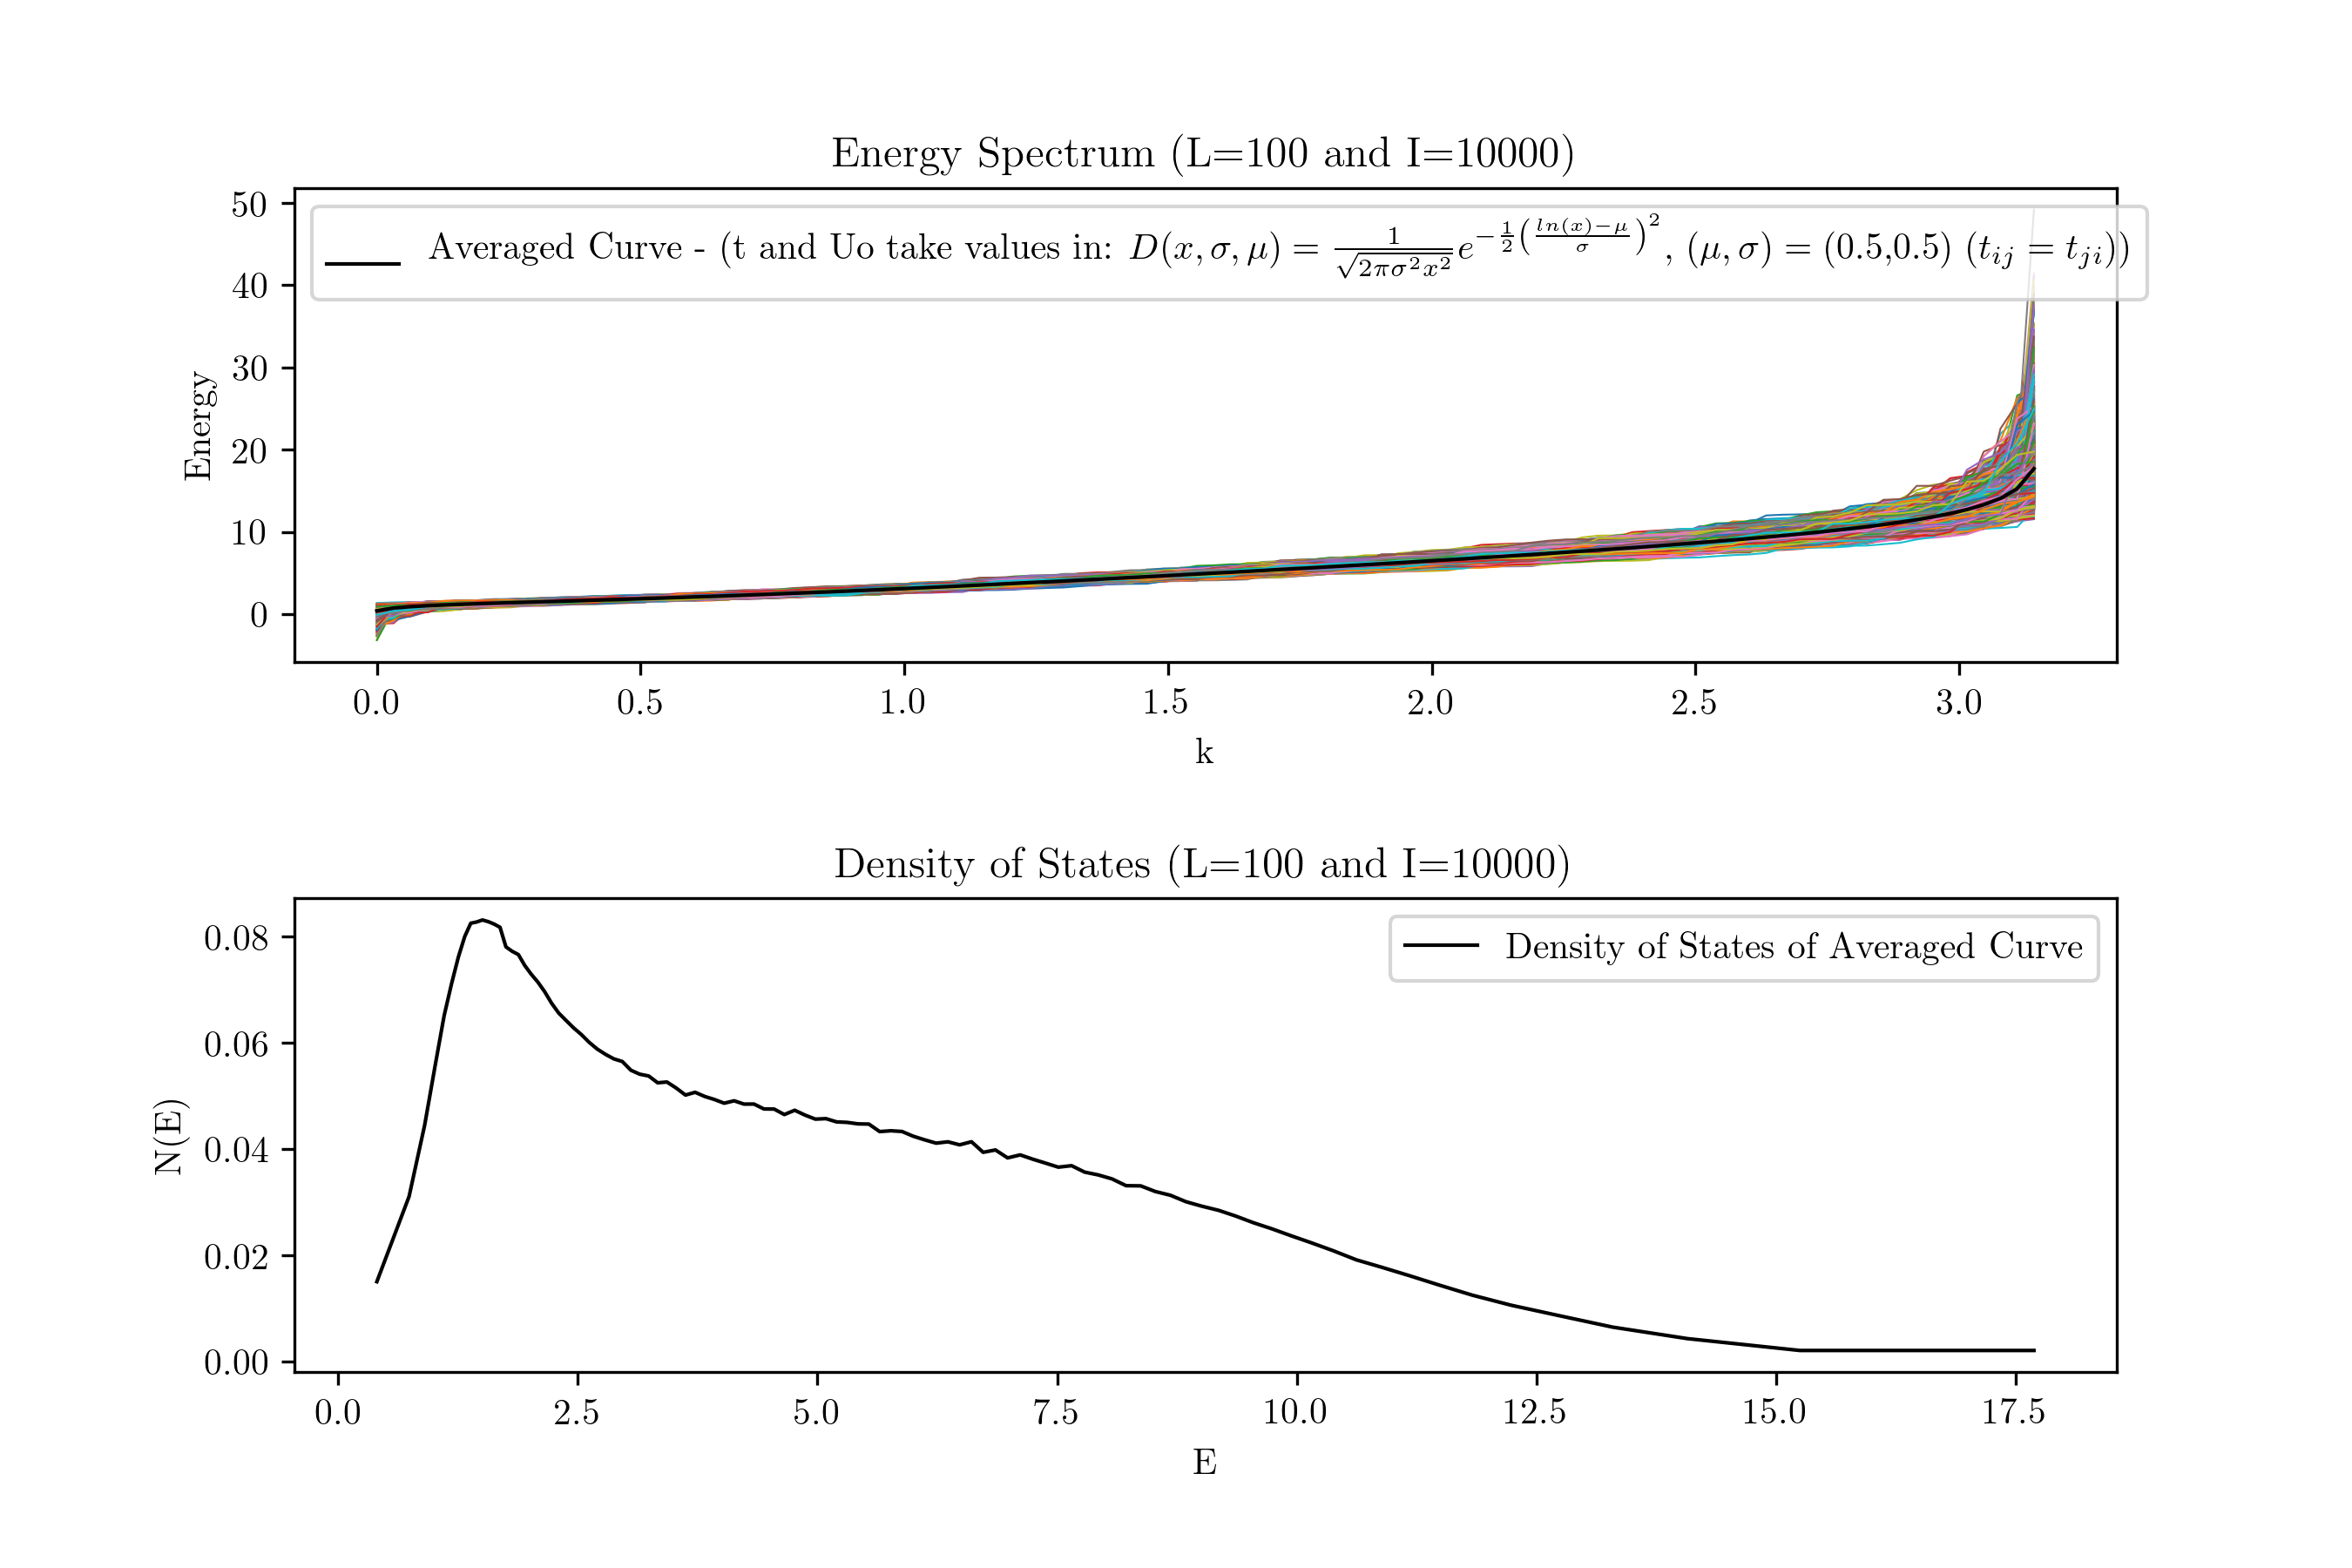
\includegraphics[scale=0.65]{EDOSRoRL.png}
                \caption{Energy Spectrum and DoS, $U_{0}$ and hopping terms $t$ take values in a log-normal distribution.}
                \label{f7a}
        \end{subfigure}
        \begin{subfigure}[b]{\textwidth}
        		\centering
                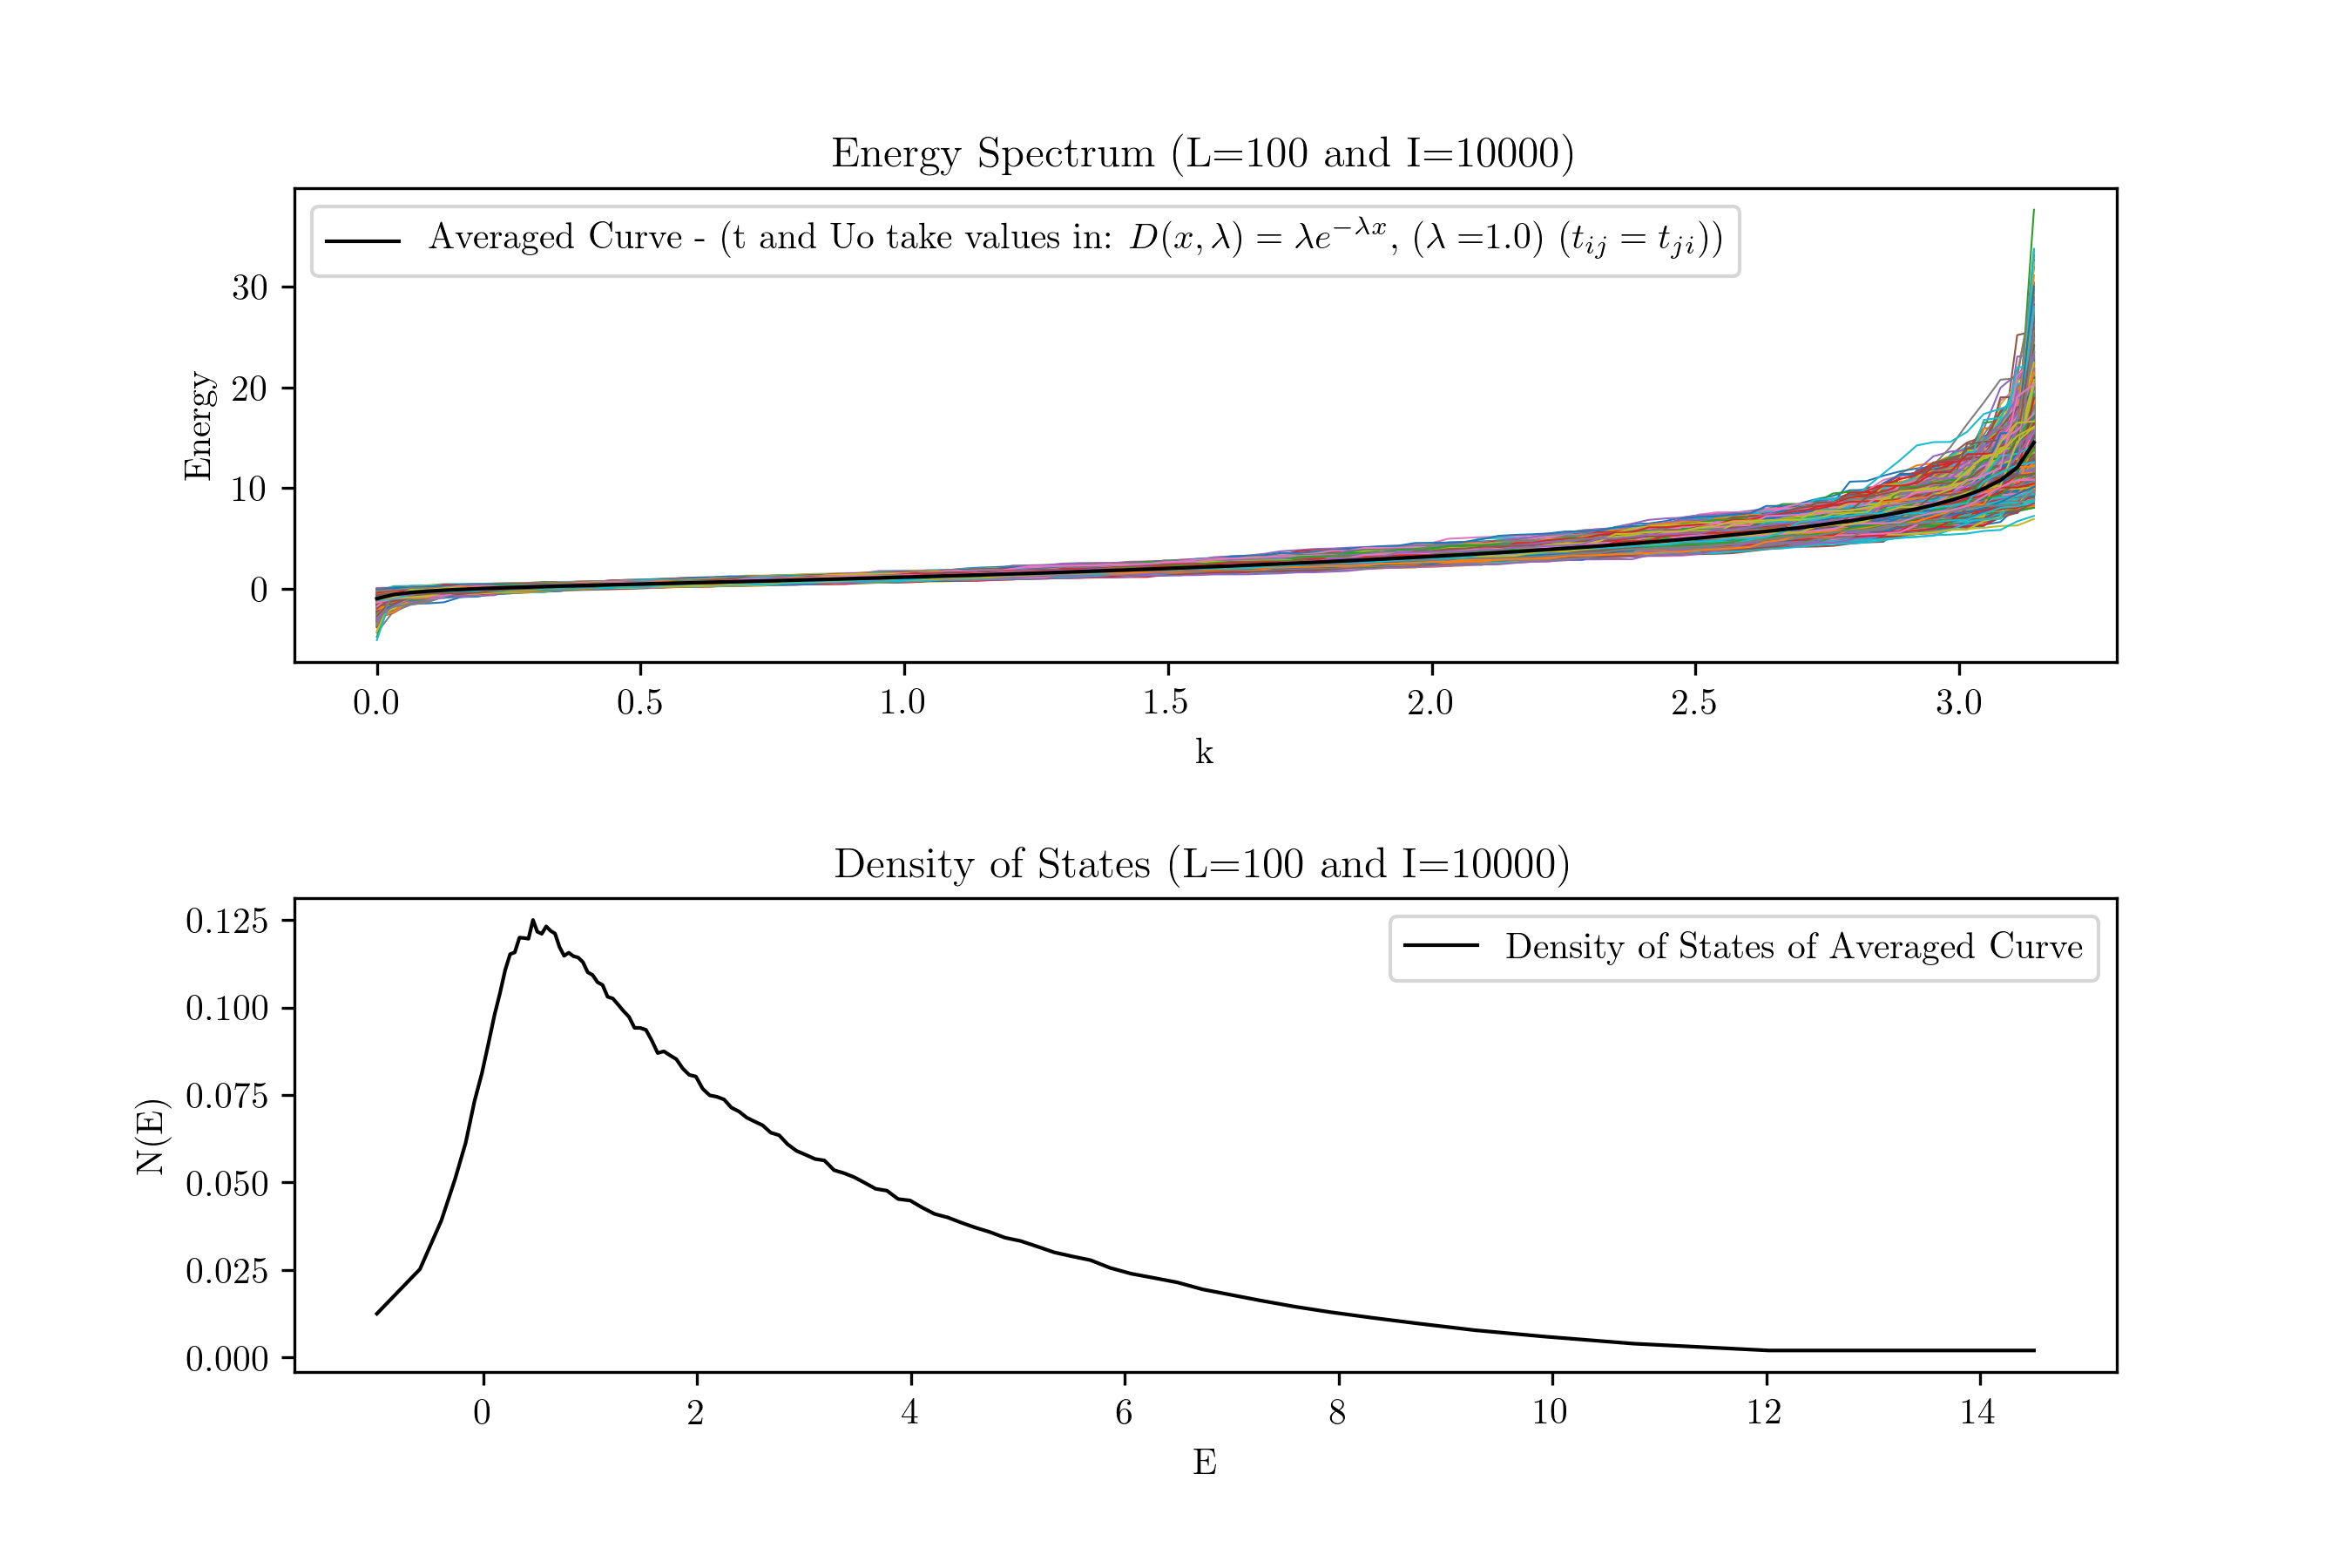
\includegraphics[scale=0.65]{EDOSRoRE.png}
                \caption{ Energy Spectrum and DoS, $U_{0}$ and hopping terms $t$ take values in an inverse-exponential distribution.}
                \label{f7b}
        \end{subfigure}
        \caption{Chain of 100 sites and 10000 iterations, $U_{0}$ and hopping terms $t$ take values in: (a) log-normal distribution and (b) inverse-exponential distribution.}
        \label{f7}
\end{figure}

\clearpage
\subsection{Numerical Current Calculation}

The current calculation depends on different parameters, for this reason it is useful understand how variations in the parameters can affect the computed current. First it is considered the case in which the width of the gap vary. After consider the variation of parameters as the on-site potential or the hopping terms, the most significant parameter that changes the width of the gap was identified as the Fermi energy $ef$. Figure \ref{fcurr} shows the variation of the Fermi energy in terms of the initially defined $ef$. The change in the value of the Fermi energy can be simulated with the impurity level of the chain; thus by including impurities in the chain, the width of the gap can be controlled.

\begin{figure}[ht]
    \centering
    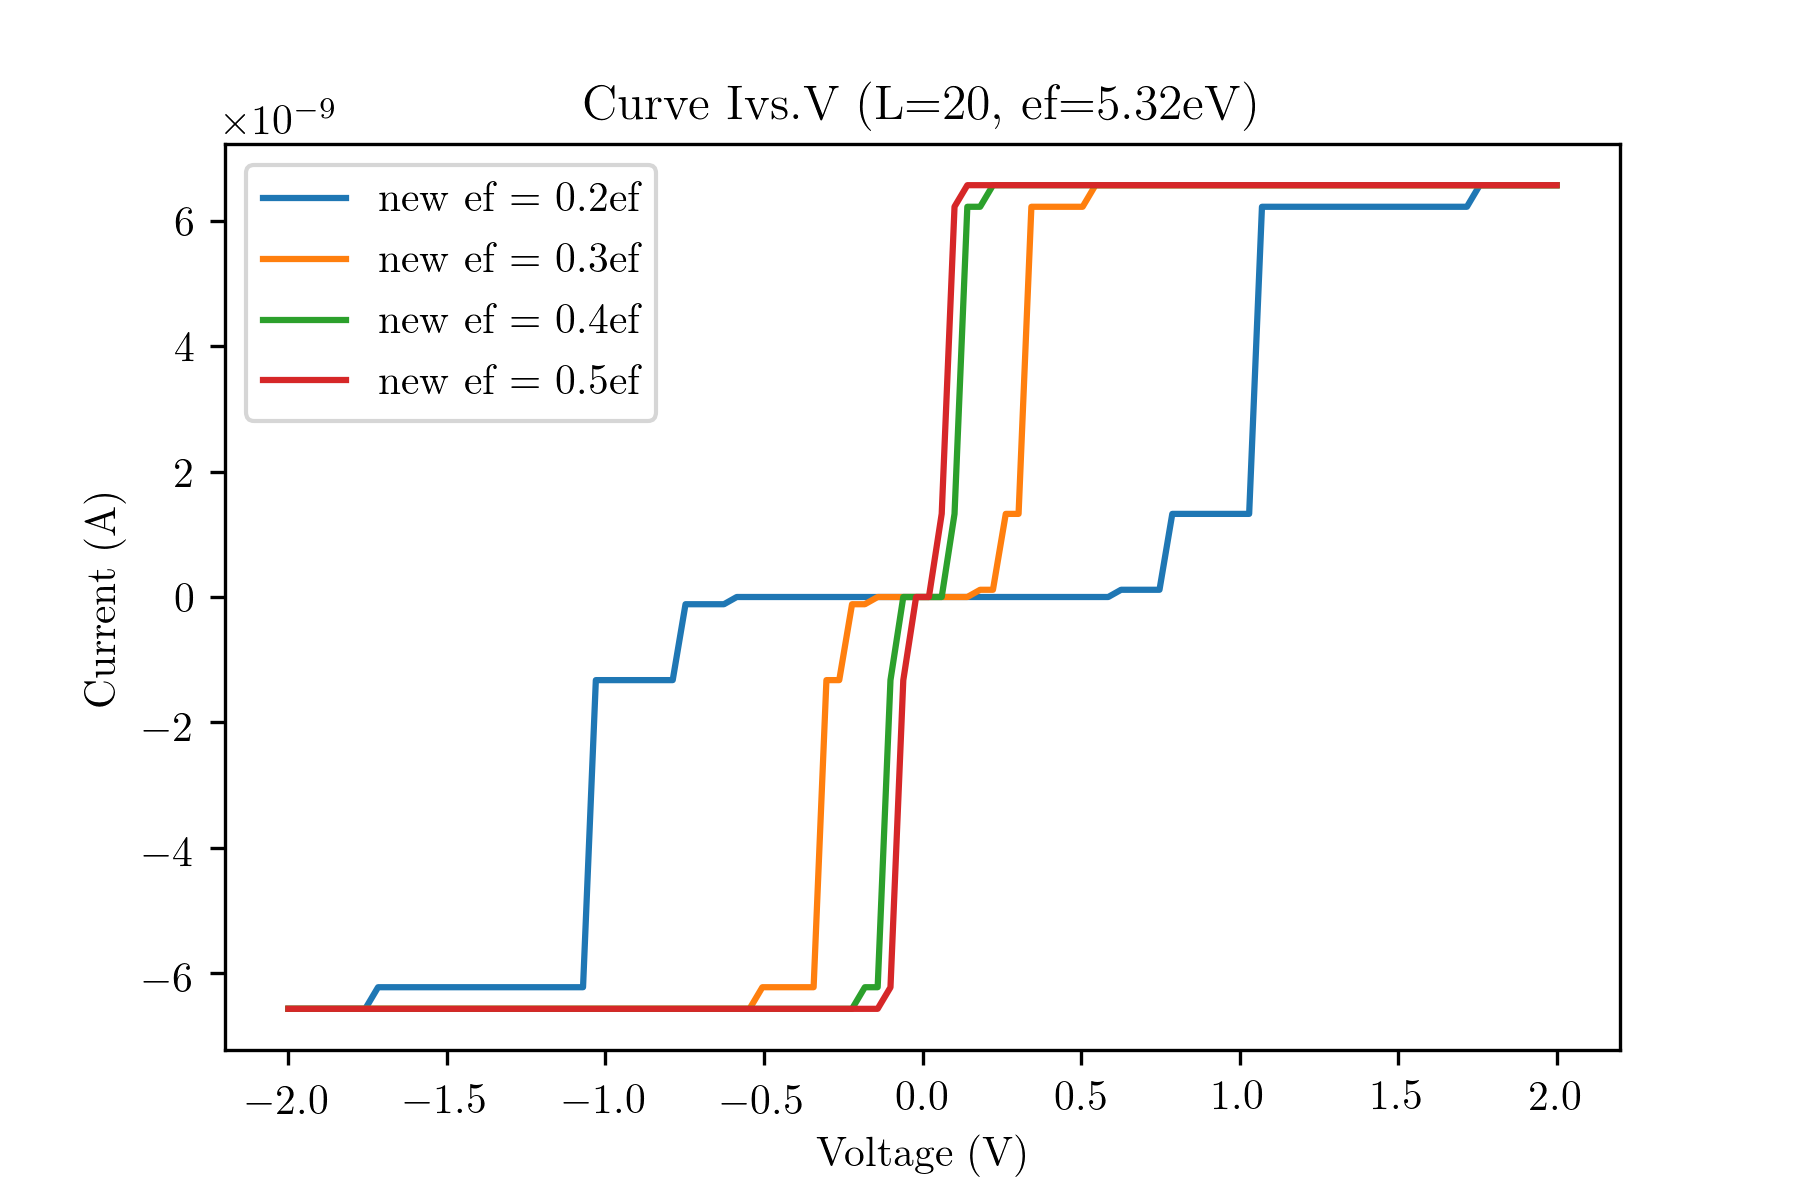
\includegraphics[scale=0.75]{Current.png}
    \caption{Currents obtained by varying the Fermi energy.}
    \label{fcurr}
\end{figure}

On the other hand, it was studied how the variation of the parameter $\kappa$ which describes the unbalance of potential between the reservoirs, affect the computed current. According to Figure \ref{fvark}, the effect of vary $\kappa$ is a displacement of the curve. In addition, the critical cases when $\kappa = 0$ or $\kappa = 1$ show that the only contribution of the current is due to one of the two reservoirs.

\begin{figure}[ht]
    \centering
    \includegraphics[scale=0.75]{Vark.png}
    \caption{Currents obtained by varying the voltage unbalance constant $\kappa$.}
    \label{fvark}
\end{figure}

\clearpage
\newpage
\section{Russek Model of Stochastic Josephson Junctions}

The model proposed by Russek\cite{RUSSEK} is a RCSJ model with a thermal noise contribution. According to Russek, a Josephson Junction can be modelled as a parallel circuit of a normal-state resistance (the measured resistance when the junction is not in the superconducting state), the capacitance of the junction, a superconducting current and a noise current due to thermal fluctuations. 
 
\begin{figure}[ht]
    \centering
    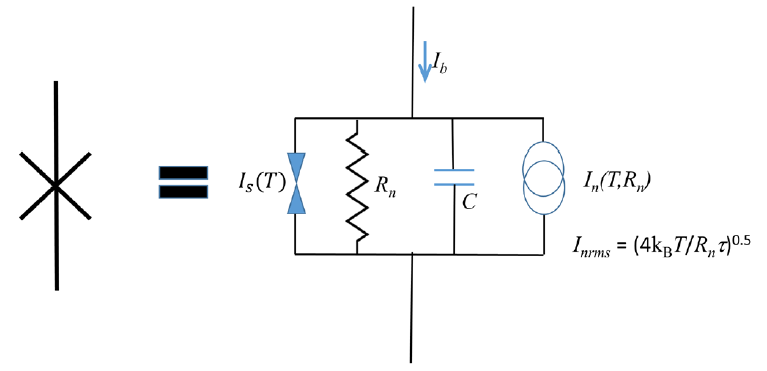
\includegraphics[scale=0.6]{Circuit.png}
    \caption{Josephson Junction circuit representation.}
    \label{CircuitJJ}
\end{figure}

If we consider that a bias current $I_{b}$ is applied to the circuit, by conservation of the current in the circuit nodes, we can obtain the equation:
$$
	I_{b} = I_{n}(T,R_{n}) + Is(T) + C\frac{dV}{dt} + \frac{V}{R_{n}}
$$
Consider a time-dependent noise with $I_{nrms} = \sqrt{4k_{b}T / R_{n}\tau}$\footnote{The rms value is obtained by integrating $I_{nrms} = \sqrt{\frac{1}{\tau}\int_{t_{0}}^{t_{0}+\tau} I_{n}^{2}(t) dt}$}, the superconducting current as a function of the change of phase of the order parameter across the junction $\theta$, $I_{s} = I_{c} \sin{\theta}$ with $Ic$ the superconducting critical current, and a derivative phase-dependent voltage $V = \frac{\Phi_{0}}{2\pi}\dot{\theta}$. Then, the current equation can be written as:

\begin{equation}
I_{b} = I_{n}(T,R_{n}, t) + I_{c}\sin{\theta} + C\frac{\Phi_{0}}{2\pi}\ddot{\theta} + \frac{\Phi_{0}}{2\pi R_{n}}\dot{\theta}
\end{equation}
\label{currents}


\subsection{RSJ Model}
The I-V curve for the Schneider synapse is well fitted to the RSJ model. That special case can be derived from Equation \ref{currents} by making $C=0$ and $I_{n}=0$, then the expression is reduced to:

\begin{equation}
I_{b} =  I_{c}\sin(\theta) + \frac{\Phi_{0}}{2\pi R_{n}}\dot{\theta}
\end{equation}
\label{rsj}

If we define $\tau = \frac{t}{\left(\frac{\Phi_{0}}{2\pi R_{n}I_{c}}\right)}$, and $I = \frac{Ib}{Ic}$, the Equation \ref{rsj} becomes:
$$
	\frac{I_{b}}{I_{c}} = \sin(\theta) + \frac{\Phi_{0}}{2\pi R_{n} I_{c}}\frac{d\theta}{dt} = \frac{\Phi_{0}}{2\pi R_{n} I_{c}}\left(\frac{d\theta}{d\tau} \frac{d\tau}{dt}\right) = \sin(\theta) + \frac{\Phi_{0}}{2\pi R_{n} I_{c}}\frac{d\theta}{d\tau} \frac{2\pi R_{n} I_{c}}{\Phi_{0}}
$$
$$
	I = \frac{d\theta}{d\tau} + \sin(\theta) \longrightarrow d\tau = \frac{d\theta}{I-\sin(\theta)}
$$
By integrating this expression and choosing the integration constant $\tau_{0}$ as $0$:
$$
\tau - \tau_{0} = \tau = \int \frac{d\theta}{I-\sin(\theta)} = \frac{-2\arctan\left(\frac{1-I\tan(\theta/2)}{\sqrt{I^{2}-1}}\right)}{\sqrt{I^{2}-1}}
$$
$$
\arctan\left(\frac{I\tan(\theta/2)-1}{\sqrt{I^{2}-1}}\right)=\frac{\sqrt{I^{2}-1}}{2} \tau
$$
$$
\frac{I\tan(\theta/2)-1}{\sqrt{I^{2}-1}} = \tan\left(\frac{\sqrt{I^{2}-1}}{2}\tau\right)
$$
$$
\tan(\theta/2) = \frac{1}{I} + \frac{\sqrt{I^{2}-1}}{I}\tan\left(\frac{\tau \sqrt{I^{2}-1}}{2}\right)
$$
$$
\theta(t) = 2\arctan\left[\frac{1}{I} + \frac{\sqrt{I^{2}-1}}{I} \tan\left(\frac{\tau \sqrt{I^{2}-1}}{2}\right) \right]
$$
From the right part of the equation, we can obtain the period $T$ of the phase $\theta(t)$. We know that $\tan$ has period $\pi$ and $\tau = t(2\pi R_{n}I_{c}/\Phi_{0}) = t\gamma$ then the period of the phase can be obtain by making $t=T$ and requiring that $\tan([...]T) = \pi$:
$$
\frac{\tau\sqrt{I^{2}-1}}{2} = \frac{\gamma T \sqrt{I^{2}-1}}{2} = \pi
$$
$$
\rightarrow T = \frac{2\pi}{\gamma \sqrt{I^{2}-1}}
$$  
This period $T$ says that the phase of the order parameter changes $2\pi$ every $T$. Now we are interested in the time-average behavior of V, that is:
$$
\langle V(t)\rangle = \frac{\Phi_{0}}{2\pi}\left\langle\frac{d\theta(t)}{dt}\right\rangle = \frac{\Phi_{0}}{2\pi}\left(\frac{1}{T}\int_{0}^{T}\frac{d\theta}{dt} dt\right)
$$
Here $\frac{d\theta}{dt}$ is the change of the order parameter, then the total change of the phase between 0 and a period $T$ in $2\pi$ as said before, thus we can replace the integral by $2\pi$:
$$
\langle V(t)\rangle = \frac{\Phi_{0}}{2\pi}\left(\frac{1}{T}\int_{0}^{T}\frac{d\theta}{dt} dt\right) = \frac{\Phi_{0}}{T} = \frac{\Phi_{0}\gamma \sqrt{I^{2}-1}}{2\pi} 
$$
Replacing in this expression the original definitions of $\gamma$ and $I$, we obtain:
$$
\langle V(t)\rangle = \frac{\Phi_{0}\sqrt{(I_{b}/I_{c})^{2}-1}}{2\pi} \frac{2\pi R_{n}I_{c}}{\Phi_{0}}  = R_{n}I_{c} \sqrt{(I_{b}/I_{c})^{2}-1} 
$$ 
Finally we found an analytical expression for the average behavior of $V(t)$ when $C=0$ and the thermal noise is not considered. 

\begin{equation}
\langle V(t)\rangle = \left\{ \begin{array}{lcc}
             R_{n}I_{c} \sqrt{(I_{b}/I_{c})^{2}-1} \qquad (I_{b} \geq I_{c})
             \\ 0  \qquad $in any other case$\\
             \end{array}
   \right.
\end{equation}
\label{Analytical}

The first part of Equation \ref{Analytical} is derived from the steps shown before, however under the condition ($I_{b}<I_{c}$) has to take a value of zero for two reasons: one is because negative roots cannot be interpreted as a measure voltage and second, it is required that the bias current surpass the critical current to enter de system into the voltage state, if that is not the case, the voltage measured through the junction must be zero.

\begin{figure}[ht]
    \centering
    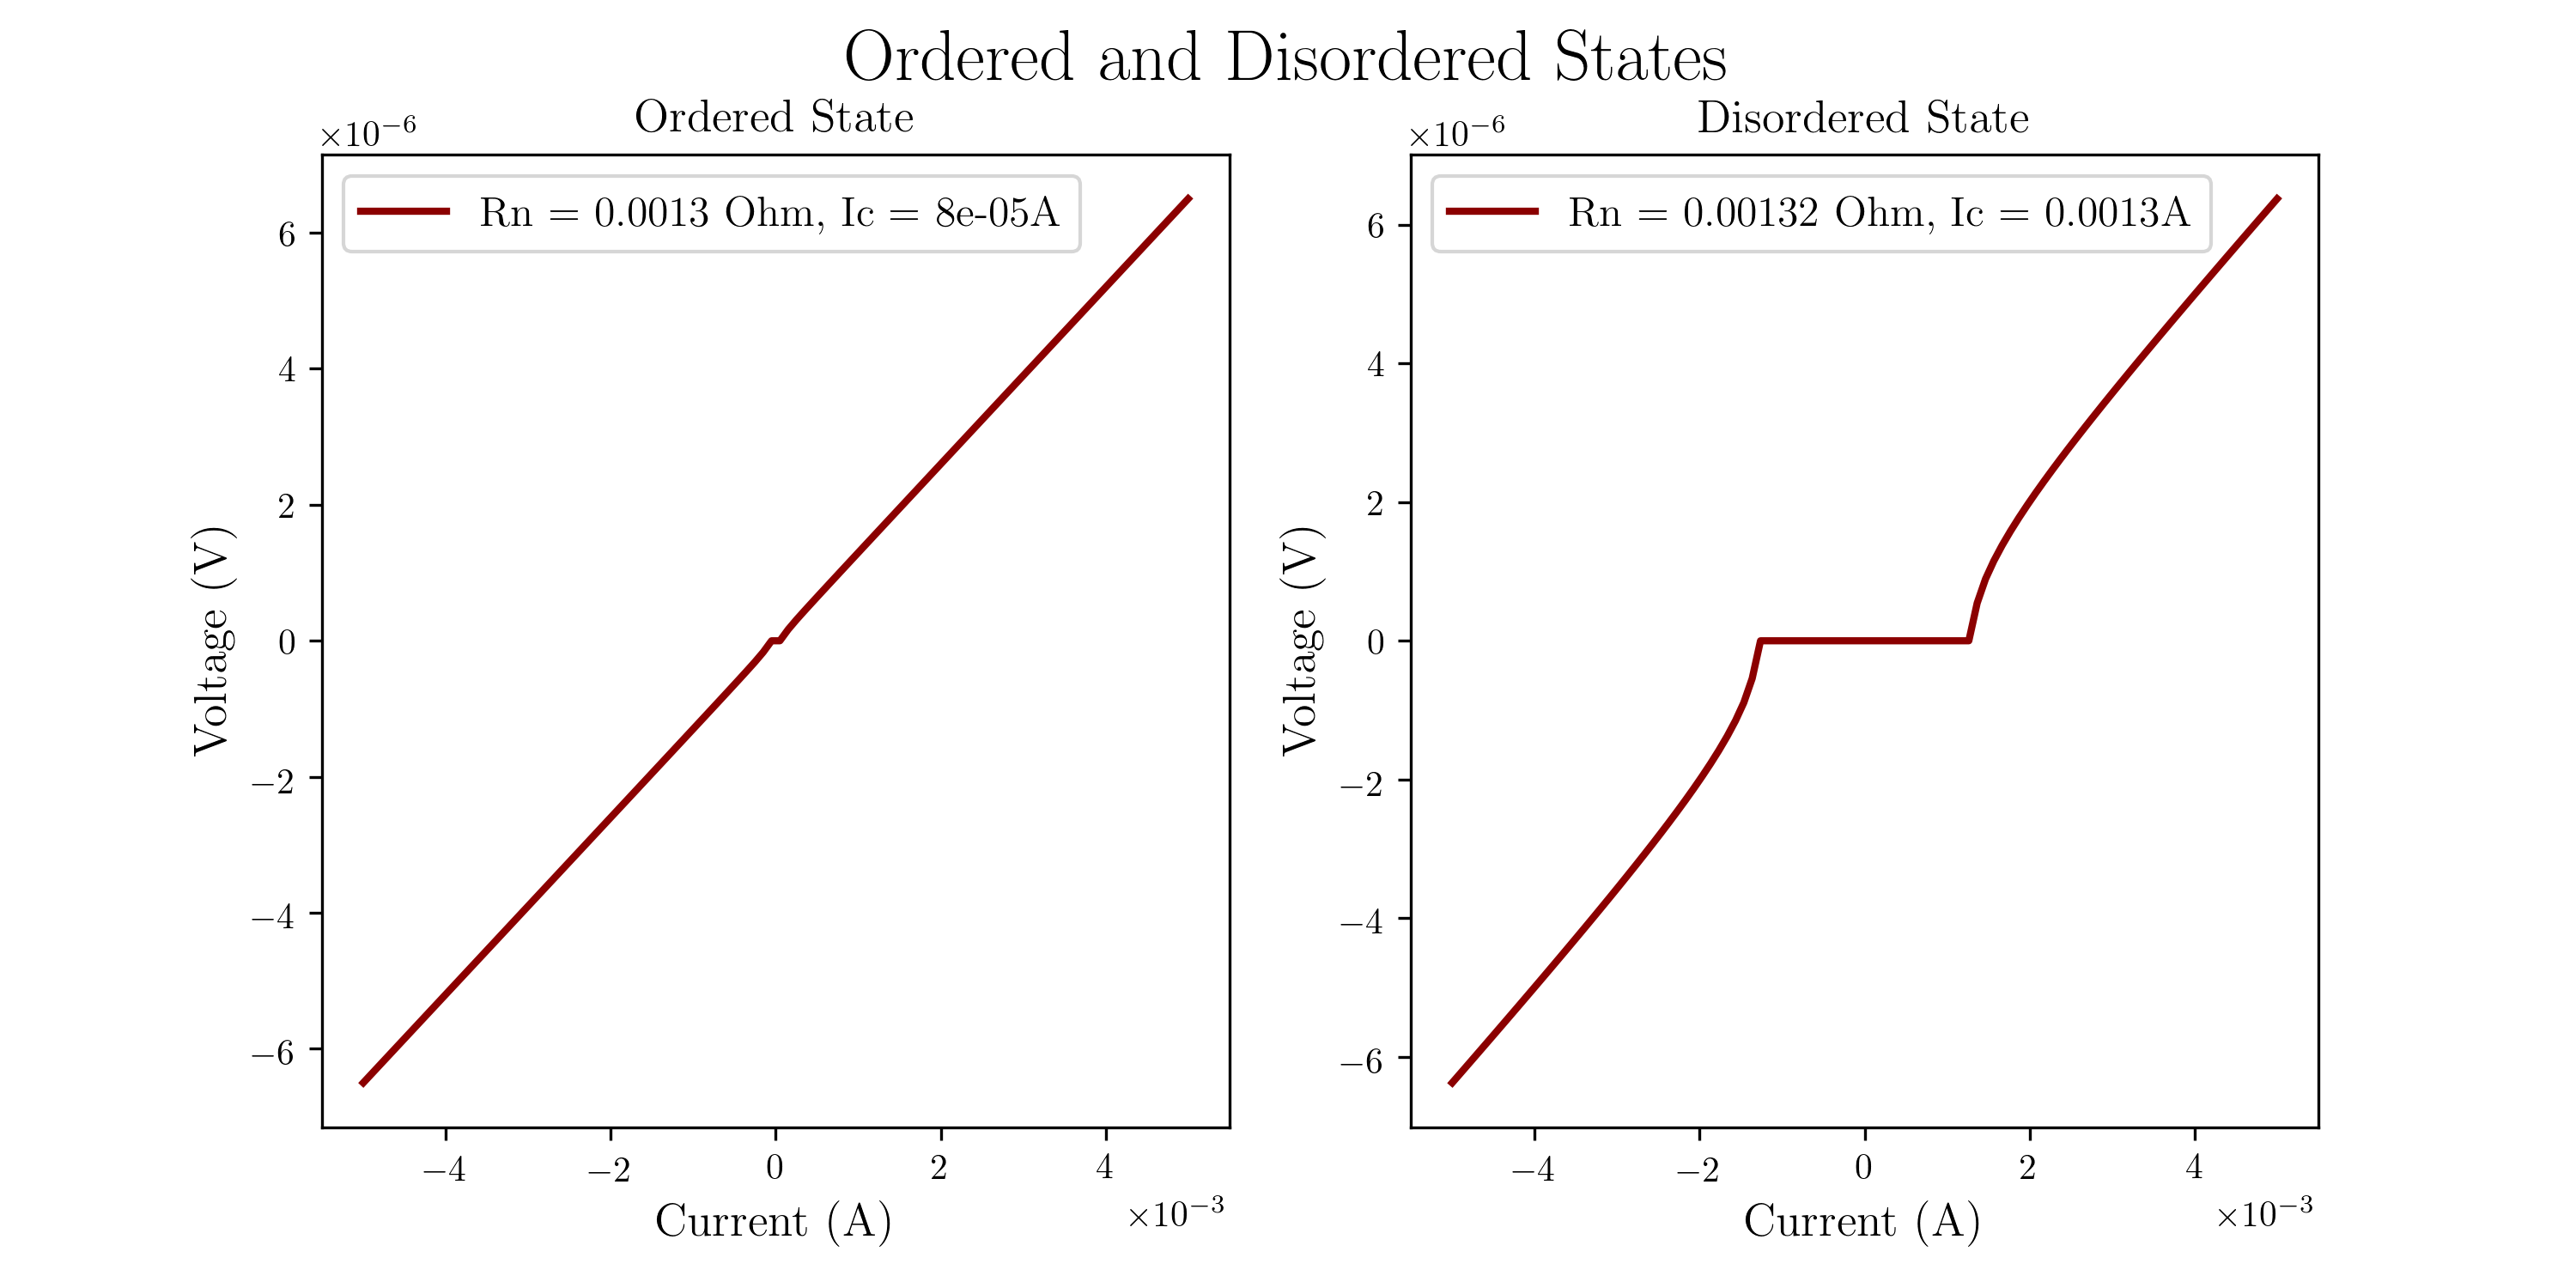
\includegraphics[scale=0.65]{AN_OrderDisorder.png}
    \caption{Plot of Voltage vs. (Bias) Current for the Equation \ref{Analytical} using the values of critical current and normal state resistance reported by Schneider et al. \cite{MAINREF}.}
    \label{AnORDIS}
\end{figure}

Note that in Figure\ref{AnORDIS},the region where a current is measure at zero voltage changes with the value of the superconducting critical current. Experimentally the value of $I_{c}$ can be tuned by applying a magnetic field and pulses of electric field. Because of this, it is necessary to consider the spiking behavior that voltage can have due to this effect.

\subsection{RSJ Model With Order Parameter Dependency}

According to Russek, one simple way to model the superconducting critical current dependency on the order parameter and the temperature is:
$$
 I_{c}(m, T) = [(1-m))I_{cv} + I_{cm}]\left[1-\left(\frac{T}{Tc}\right)^{2}\right]
$$
Where $T$ is the temperature and $m$ is the order parameter that describes the alignment of the Mn nanocluster spins between the junction. $Icm$ is the smallest critical current, and $I$

\begin{figure}[ht]
    \centering
    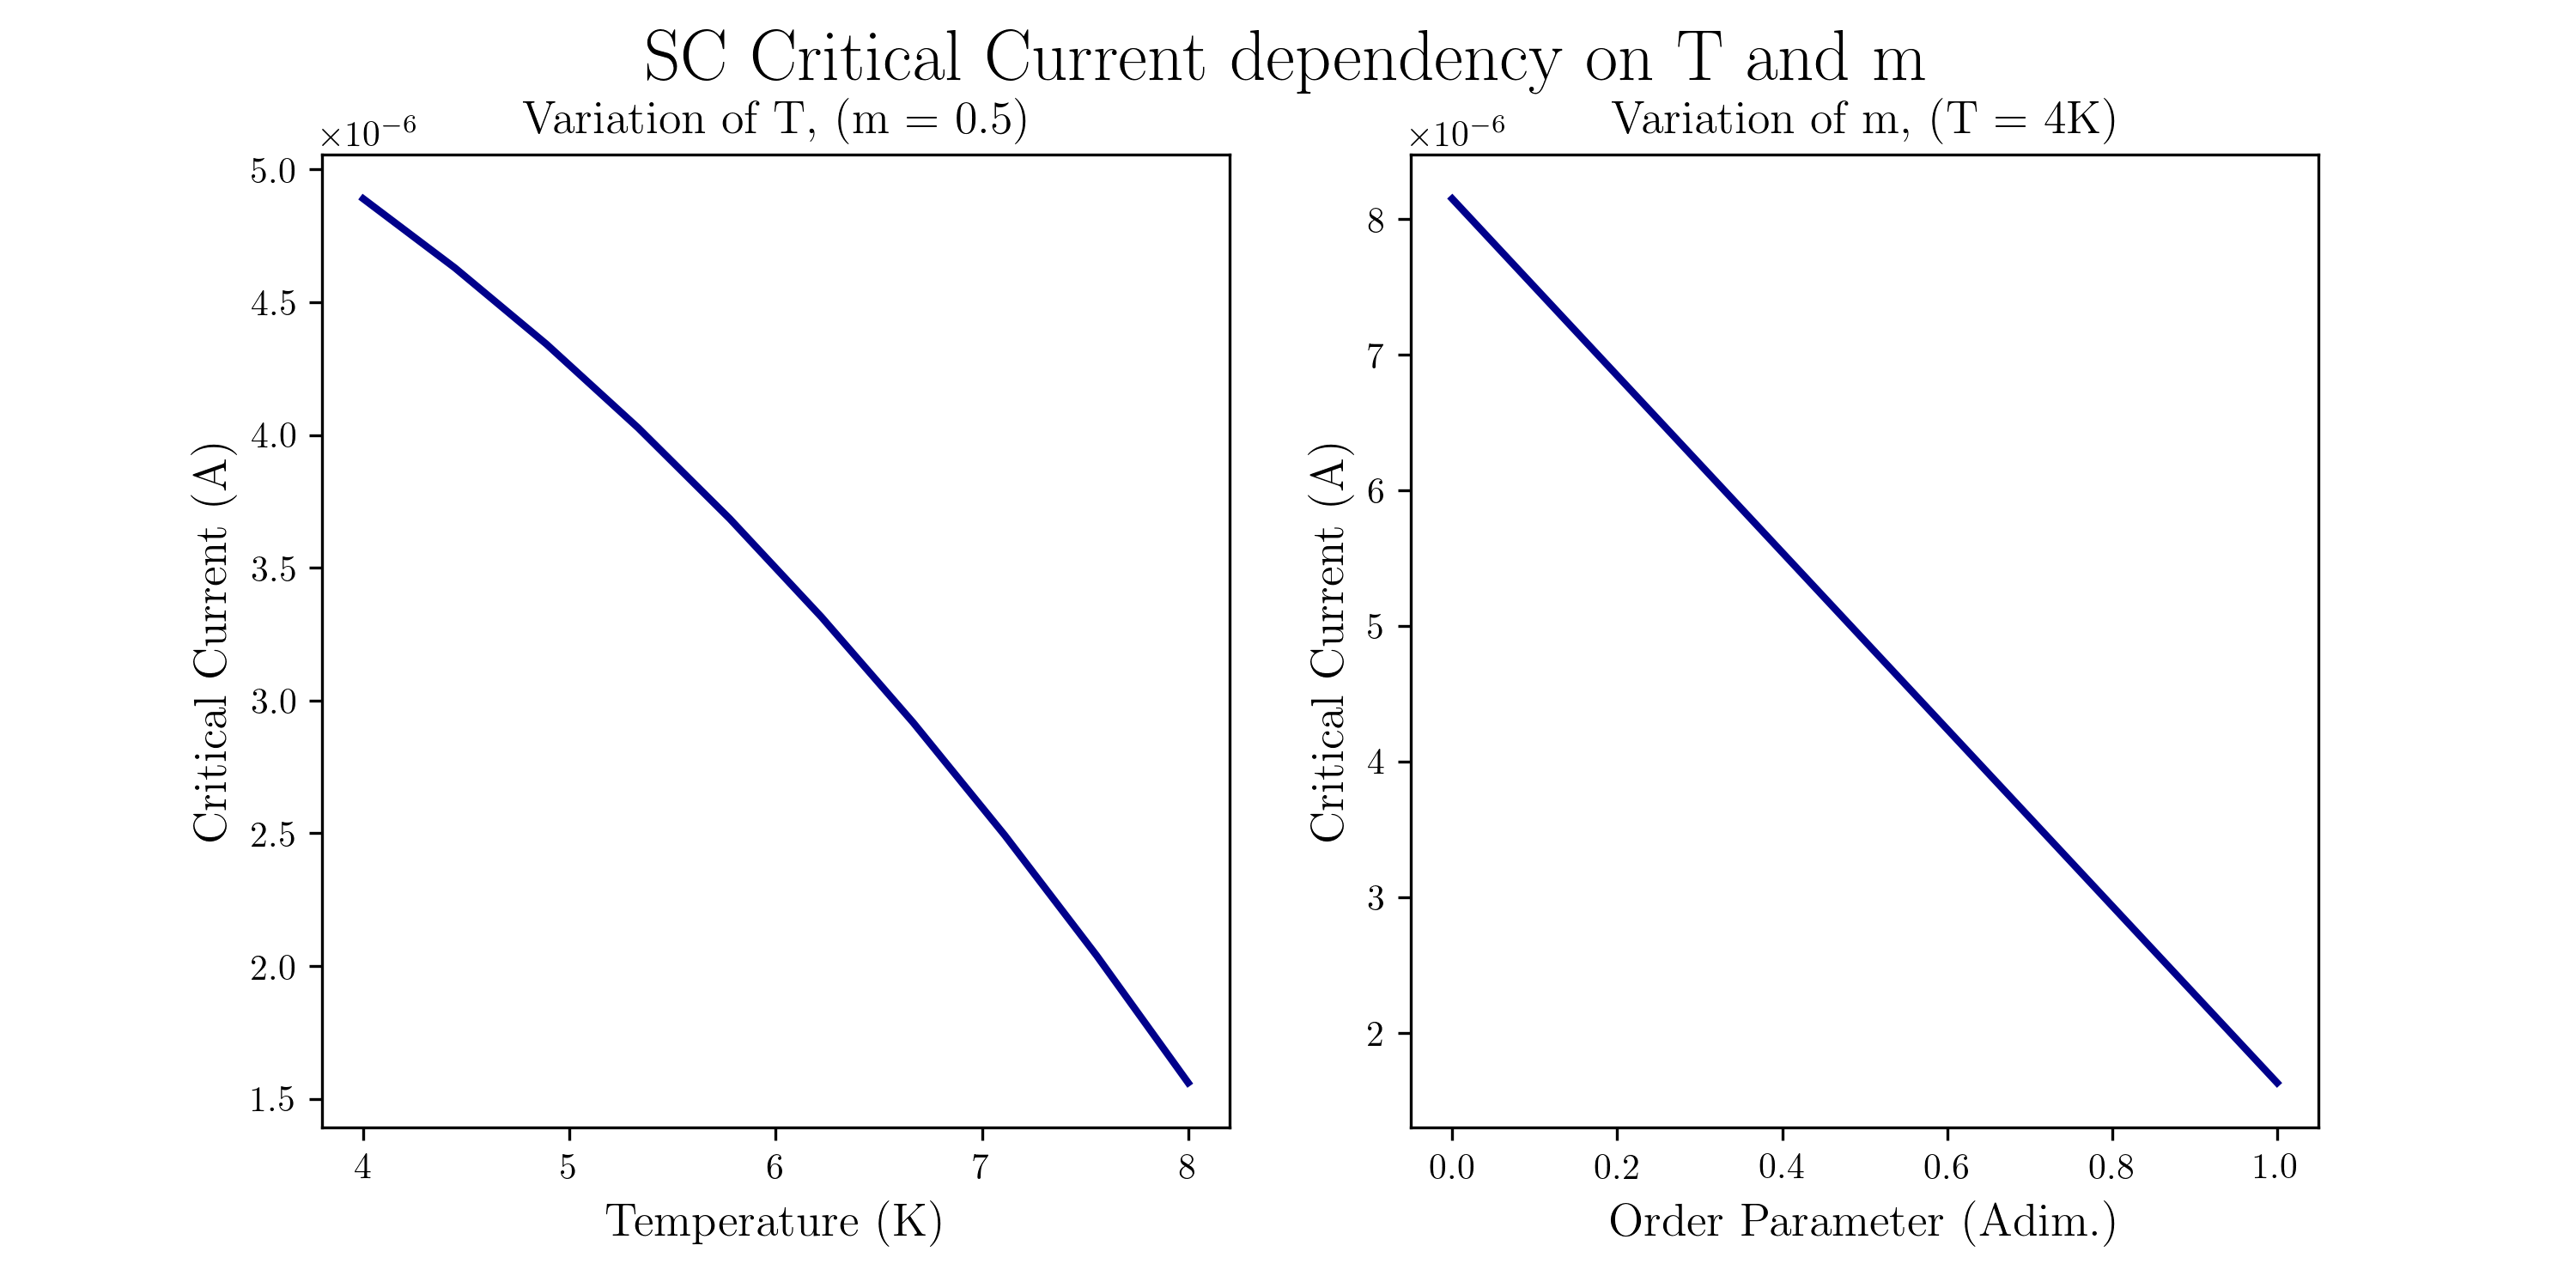
\includegraphics[scale=0.65]{SC_SCDependencyOnMT.png}
    \caption{Plot of Voltage vs. (Bias) Current for the Equation \ref{Analytical} using the values of critical current and normal state resistance reported by Schneider et al. \cite{MAINREF}.}
    \label{SC_SC}
\end{figure}

\begin{figure}[ht]
    \centering
    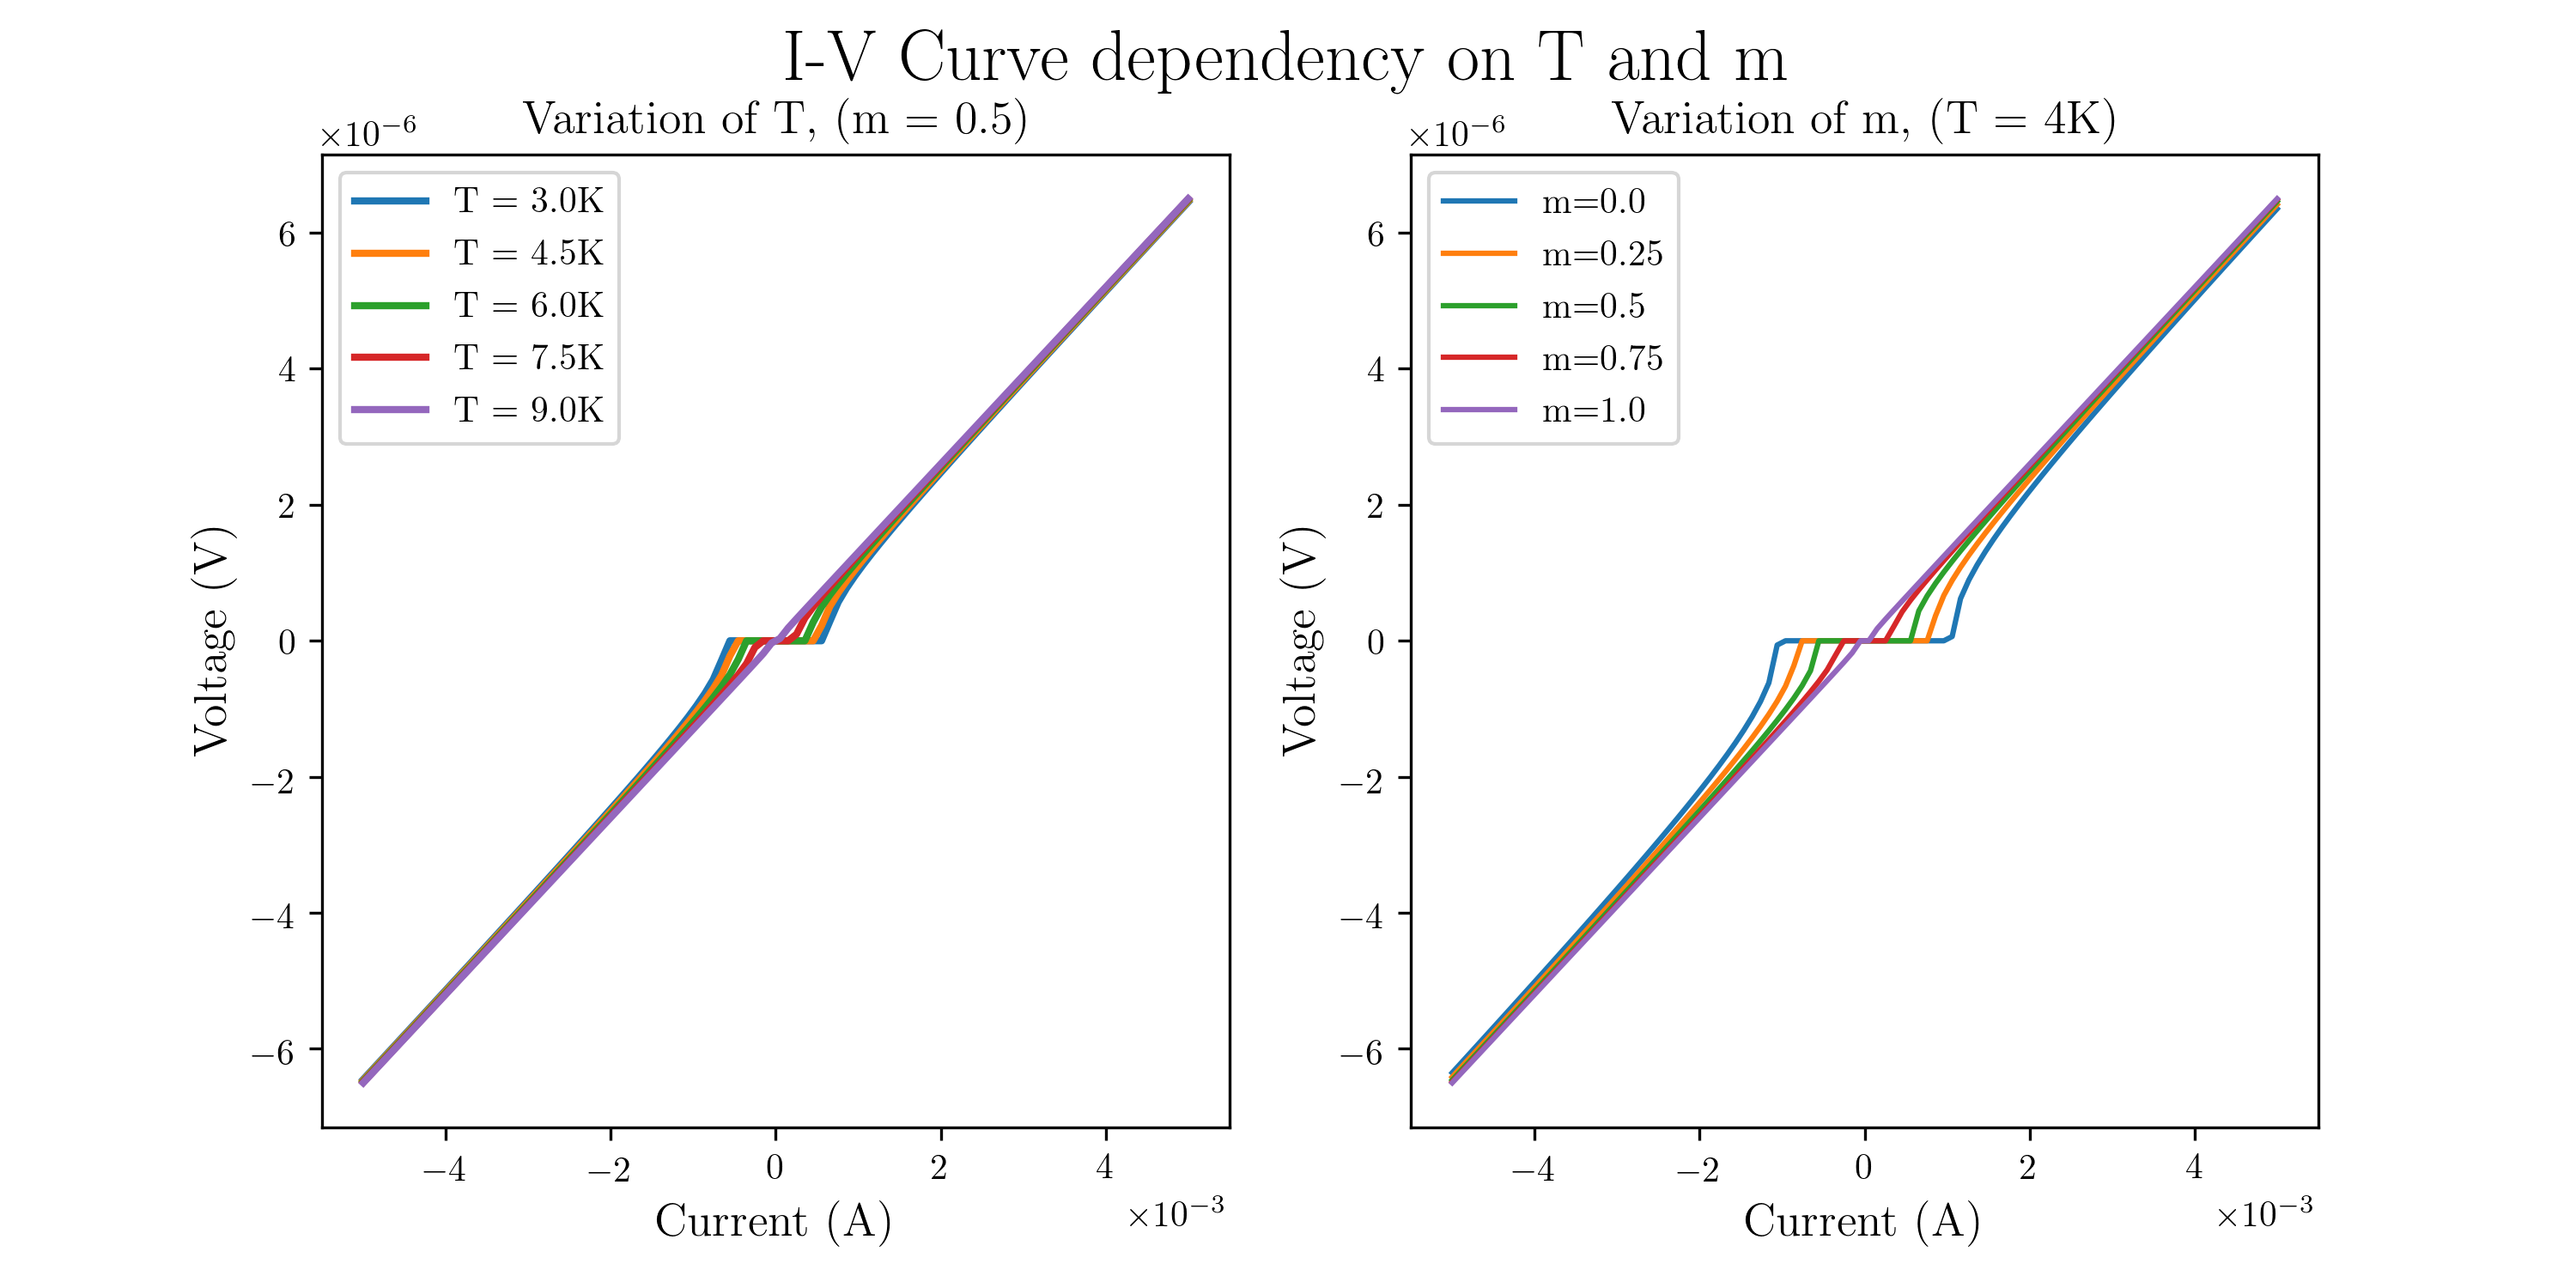
\includegraphics[scale=0.65]{IV_SCDependencyOnMT.png}
    \caption{Plot of Voltage vs. (Bias) Current for the Equation \ref{Analytical} using the values of critical current and normal state resistance reported by Schneider et al. \cite{MAINREF}.}
    \label{IV_SC}
\end{figure}

\newpage
\section{Conclusion}
\newpage
\begin{thebibliography}{10}

\bibitem{MEMRISTORS} M. Prezioso, F. Merrikh-Bayat, B. Hoskins, G. Adam, K. Likharev \& D. Strukov \textit{Training and operation of an intergrated neuromorphic network based on metal-oxide memristors}. Nature \textbf{521}, 61-64, (2015)
\bibitem{CORRIENTES} Xin-Qi Li and YiJing Yang \textit{Electrical transport through individual DNA molecules}. cond-mat 0107015 (2001).

\bibitem{CMOS} A. Graves, G. Wayne, M. Reynolds, T. Harley, I. Danihelka, A. Grabska-Barwinska, S. Colmenarejo, E. Grefenstette, T. Ramalho \& J. Agapiou \textit{Hybrid computing using a neural network with dynamical external memory}. Nature \textbf{538}, 471-476 (2016).

\bibitem{SFQ} T. Hirose, T.Asai \& Y. Amemiya \textit{Pulsed neural networks consisting of single-flux-quantum spiking neurons}. Phys. C Supercond. Appl. \textbf{463-465}, 1072-1075, (2007).

\bibitem{VARIOS} P. Merolla, J. Arthur, R. Alvarez, A. Cassidy, J. Sawada, F. Akopyan, B. Jackson \& N. Imam \textit{A million spiking-neuron integrated circuit with a scalable communication network and interface}. Science \textbf{345}, 668-673, (2014).

\bibitem{MAINREF} M. Schneider, C. Donnelly, S. Russek, B. Baek, M. Pufall, P. Hopkins, P. Dresselhaus, S. Benz \& W. Rippard:  \textit{Ultralow power artificial synapses using nanotextured magnetic Josephson junctions}. Science Advances \textbf{4}:1, (2018).

\bibitem{RUSSEK} S. Russek, C. Donnelly, M. Schneider, B. Baek, M. Pufall, W. Rippard,
P. Hopkins, P. Dresselhaus \& S. Benz: \textit{Stochastic single flux quantum neuromorphic computing using magnetically tunable Josephson junctions}. IEEE International Conference on Rebooting Computing (ICRC), San Diego, CA, 2016, pp. 1-5, (2016).

\bibitem{NISTIlus} Kelley Sean, \textit{Figure taken from NIST Animation}, 
\\ www.nist.gov/news-events/news/2018/01/nists-superconducting-synapse-may-be-missing-piece-artificial-brains
\end{thebibliography}

\end{document}

